% 자동 생성: python3 src/md2beamer.py Day1_슬라이드.md Day1_슬라이드_body.tex  (직접 고치려면 src/slide_config.py 또는 이 파일)


% ---- md slide 1: PM 트랙 Day 1 — 프로젝트 매니지먼트 일반론과 착수
\begin{frame}[allowframebreaks=1.0]{PM 트랙 Day 1 — 프로젝트 매니지먼트 일반론과 착수}
\small
\begin{itemize}
\item\relax 프로젝트 매니지먼트 4일 특강 · 1일차
\item\relax 사례 회사: ㈜온담F\&B홀딩스 ONE ONDAM 프로그램 P1 「차세대 주문·재고 통합 플랫폼 구축」
\item\relax 승인 예산 168억 원 · 2026-01-05 \textasciitilde{} 2027-05-29 · 하이브리드(스프린트 36회 + 게이트 G0\textasciitilde{}G5)
\item\relax 오늘의 세 질문: \textbf{이것은 무엇인가 / 무엇을 따를 것인가 / 어떻게 시작할 것인가}
\end{itemize}
\note{표지. 사례 회사 문서(\textsf{교재/공통/가상회사\_온담F앤B.md}) §1\textasciitilde{}§3과 §5 핵심 숫자 표를 사전에 읽어 왔는지 확인한다. 읽지 않은 수강생은 워크북 §0.3 한 페이지 요약을 4교시 전까지 읽도록 안내한다. 교재 서문 참조. 예상 소요 3분.}
\end{frame}

% ---- md slide 2: 오늘의 흐름
\begin{frame}[allowframebreaks=1.0]{오늘의 흐름}
\small
{\usebeamercolor[fg]{normal text}\footnotesize\setlength{\tabcolsep}{3pt}\renewcommand{\arraystretch}{1.12}
\begin{tabular}{@{}>{\raggedright\arraybackslash}p{0.134\textwidth}>{\raggedright\arraybackslash}p{0.134\textwidth}>{\raggedright\arraybackslash}p{0.584\textwidth}>{\raggedright\arraybackslash}p{0.134\textwidth}@{}}
\toprule
\textbf{블록} & \textbf{시간} & \textbf{내용} & \textbf{교재} \\
\midrule
1교시 & 90분 & 용어 정리 · 프로젝트란 무엇인가 · 왜 실패하는가 & 제1장 \\
2교시 & 90분 & 표준의 지형 — PMBOK 6$\rightarrow$7$\rightarrow$8, PRINCE2, ISO, 테일러링 & 제2장 \\
점심 &  &  &  \\
3교시 & 90분 & 착수 이론 — 비즈니스 케이스 · 편익 소유 · 헌장 · 이해관계자 & 제3장 전반 \\
4교시 & 90분 & \textbf{실습 ①} 온담 P1 비즈니스 케이스 요약 + 헌장 & 워크북 §1\textasciitilde{}2 \\
5교시 & 75분 & 거버넌스 · 권한 없는 PM · 프리모템 · 분야별 착수 노하우 & 제3장 후반 \\
6교시 & 75분 & \textbf{실습 ②} 이해관계자 등록부 · RACI · 프리모템 & 워크북 §3\textasciitilde{}5 \\
마무리 & 30분 & 학술 배경 깊이 읽기 · 읽을 자료 · Day2 예고 & 제4\textasciitilde{}5장 \\
\bottomrule
\end{tabular}}
\par\smallskip
\note{오전은 이론(제1\textasciitilde{}2장), 오후는 착수 이론과 실습이 번갈아 온다. 실습 ①(4교시)은 비즈니스 케이스 요약과 헌장, 실습 ②(6교시)는 등록부·RACI·프리모템이다. 오늘 만든 다섯 산출물이 Day2 계획 산출물의 입력이 된다는 점을 미리 말해 둔다. 예상 소요 3분.}
\end{frame}

% ---- md slide 3: 학습 목표 — 오늘이 끝나면
\begin{frame}[allowframebreaks=1.0]{학습 목표 — 오늘이 끝나면}
\small
\begin{itemize}
\item\relax 프로젝트·프로그램·운영을 \textbf{돈과 권한의 언어}로 구분하고, 온담 ONE ONDAM이 왜 프로그램인지 설명할 수 있다
\item\relax CHAOS 수치와 Flyvbjerg 수치를 \textbf{왜 그대로 인용하면 안 되는지} 근거를 들어 말할 수 있다
\item\relax PMBOK 6$\rightarrow$7$\rightarrow$8판의 계보를 알고, 사내 표준을 \textbf{재매핑 대장} 네 칸으로 대응시킬 수 있다
\item\relax 테일러링의 기준이 \textbf{되돌림 비용}임을 이해하고 P1과 P2에 다른 방법을 처방할 수 있다
\item\relax 비즈니스 케이스의 결함을 목록화하고, \textbf{편익 오너가 PM이 아닌 이유}를 설명할 수 있다
\item\relax 헌장 15개 항목 · 이해관계자 3속성 7유형 · RACI · 프리모템을 온담 P1으로 \textbf{직접 작성}할 수 있다
\end{itemize}
\note{여섯 개 목표 중 앞의 넷은 오전 이론, 뒤의 둘은 오후 실습에 대응한다. "기초는 다루지 않는다"는 교재 전제(주니어 PM과 3\textasciitilde{}7년차 혼합)를 명시하고, 이 과정은 자격시험 수업이 아니라는 점을 말한다. 교재 서문·제4장 4.1 방향 5(성찰적 실무자) 참조. 예상 소요 3분.}
\end{frame}

\section{1교시 (90분) — 프로젝트란 무엇인가, 왜 실패하는가}

% ---- md slide 4: 이 교시에서 배우는 것
\begin{frame}[allowframebreaks=1.0]{이 교시에서 배우는 것}
\small
\begin{itemize}
\item\relax 이 과정에서 "PM"이 무엇을 뜻하는지 — 프로젝트 매니저 / PO / 프로덕트 매니저의 3중 충돌 정리
\item\relax 프로젝트·프로그램·포트폴리오·운영 — 세 표준의 정의를 나란히 놓으면 보이는 것 [§1.1]
\item\relax 프로젝트는 왜 실패하는가 — 통계를 그대로 믿으면 안 되는 이유 [§1.2]
\item\relax 프로젝트를 임시조직으로 본다는 것 [§1.3]
\item\relax 프로젝트 유형은 하나가 아니다 — NTCP 다이아몬드 [§1.4]
\item\relax 분야별 대조 — 같은 단어, 다른 리듬, 다른 되돌림 비용 [§1.5]
\end{itemize}
\note{제1장 전체를 90분에 다룬다. 시간 배분은 용어 정리 5분, §1.1 15분, §1.2 25분, §1.3 15분, §1.4 15분, §1.5 10분, 정리 5분. §1.2(실패 통계)가 가장 길다 — 경력자가 가장 많이 틀리는 지점이기 때문이다. 예상 소요 2분.}
\end{frame}

% ---- md slide 5: 용어 정리 — 이 과정에서 "PM"은 프로젝트 매니저다
\begin{frame}[allowframebreaks=1.0]{용어 정리 — 이 과정에서 "PM"은 프로젝트 매니저다}
\small
{\usebeamercolor[fg]{normal text}\small\setlength{\tabcolsep}{3pt}\renewcommand{\arraystretch}{1.12}
\begin{tabular}{@{}>{\raggedright\arraybackslash}p{0.106\textwidth}>{\raggedright\arraybackslash}p{0.207\textwidth}>{\raggedright\arraybackslash}p{0.477\textwidth}>{\raggedright\arraybackslash}p{0.194\textwidth}@{}}
\toprule
\textbf{약칭} & \textbf{원어} & \textbf{책임지는 것} & \textbf{이 과정에서의 위치} \\
\midrule
\textbf{PM} & Project Manager & 정해진 사양·일정·예산 안에서 \textbf{산출물(output)}을 인도 & \textbf{PM 트랙 4일 (오늘)} \\
PO & Product Owner (Scrum 역할) & 백로그의 우선순위, 스프린트 단위의 가치 판단 & Product 트랙에서 다룸 \\
프로덕트 매니저 & Product Manager & 제품의 존재 이유, 시장·사용자·수명 전체의 \textbf{성과(outcome)} & Product 트랙 4일 \\
\bottomrule
\end{tabular}}
\par\smallskip
\begin{itemize}
\item\relax 한국 기업에서 세 역할이 "PM"이라는 같은 글자로 불리면서 충돌한다 — 명함이 아니라 \textbf{무엇에 책임지는가}로 구분한다
\item\relax 오늘 이후 "PM"은 온담 P1의 발주사 프로젝트 매니저(여러분)를 가리킨다
\end{itemize}
\note{이 슬라이드는 혼합 기수를 위한 오리엔테이션이며 교재 본문 밖이다. 깊이 들어가지 말고, "output은 PM의 책임, outcome은 사업 오너의 책임"이라는 3교시 §3.1 ITO 모델의 예고편으로만 쓴다. 산출물/성과의 구분이 오늘 반복해서 나온다는 것만 심어 둔다. 예상 소요 5분.}
\end{frame}

% ---- md slide 6: 프로젝트·프로그램·포트폴리오 — 세 표준의 정의
\begin{frame}[allowframebreaks=1.0]{프로젝트·프로그램·포트폴리오 — 세 표준의 정의}
\small
{\usebeamercolor[fg]{normal text}\footnotesize\setlength{\tabcolsep}{3pt}\renewcommand{\arraystretch}{1.12}
\begin{tabular}{@{}>{\raggedright\arraybackslash}p{0.129\textwidth}>{\raggedright\arraybackslash}p{0.283\textwidth}>{\raggedright\arraybackslash}p{0.305\textwidth}>{\raggedright\arraybackslash}p{0.268\textwidth}@{}}
\toprule
\textbf{표준} & \textbf{프로젝트} & \textbf{프로그램} & \textbf{포트폴리오} \\
\midrule
\textbf{ISO 21502:2020} & 합의된 목표를 위한 임시적 노력. 시작·끝이 정의됨 & 개별 관리로는 얻을 수 없는 \textbf{편익}을 위해 함께 관리 & 전략 목표를 위한 프로젝트·프로그램·\textbf{운영}의 집합 \\
\textbf{PMBOK 8판} (2025) & 고유한 산출물을 위한 임시적 노력 + \textbf{가치} 인도 & 편익과 통제를 위해 조정 관리 & 전략 목표를 위한 그룹 관리 \\
\textbf{MSP 5판} (2020) & 산출물(outputs)을 만드는 것 & outputs $\rightarrow$ capabilities $\rightarrow$ outcomes $\rightarrow$ \textbf{benefits} & (MoP가 다룸) \\
\bottomrule
\end{tabular}}
\par\smallskip
\begin{itemize}
\item\relax 공통 단어 셋: \textbf{임시적(temporary)} — 짧다는 뜻이 아니라 \textbf{끝이 정의되어 있다}는 뜻 / \textbf{편익(benefits)} / \textbf{전략·운영}
\item\relax 정의는 개념 논쟁이 아니다 — 프로젝트라 부르는 순간 예산·책임자·해산이 생기고, 운영이라 부르면 연간 예산 안에서 반복된다
\end{itemize}
\note{§1.1 개념. "누가 돈을 대고 누가 책임지는가"의 논쟁임을 먼저 말한다. outputs$\rightarrow$capabilities$\rightarrow$outcomes$\rightarrow$benefits 네 단어 사슬은 오늘 하루 종일 반복되므로 칠판에 남겨 둔다. PRINCE2 7의 정의("비즈니스 케이스에 따라 … 만들어진 임시조직")도 언급 — "임시조직"과 "비즈니스 케이스"가 §1.3과 §3.1의 예고다. 예상 소요 8분.}
\end{frame}

% ---- md slide 7: 온담으로 읽기 — ONE ONDAM은 프로그램이다
\begin{frame}[allowframebreaks=1.0]{온담으로 읽기 — ONE ONDAM은 프로그램이다}
\small
\begin{center}\usebeamercolor[fg]{normal text}
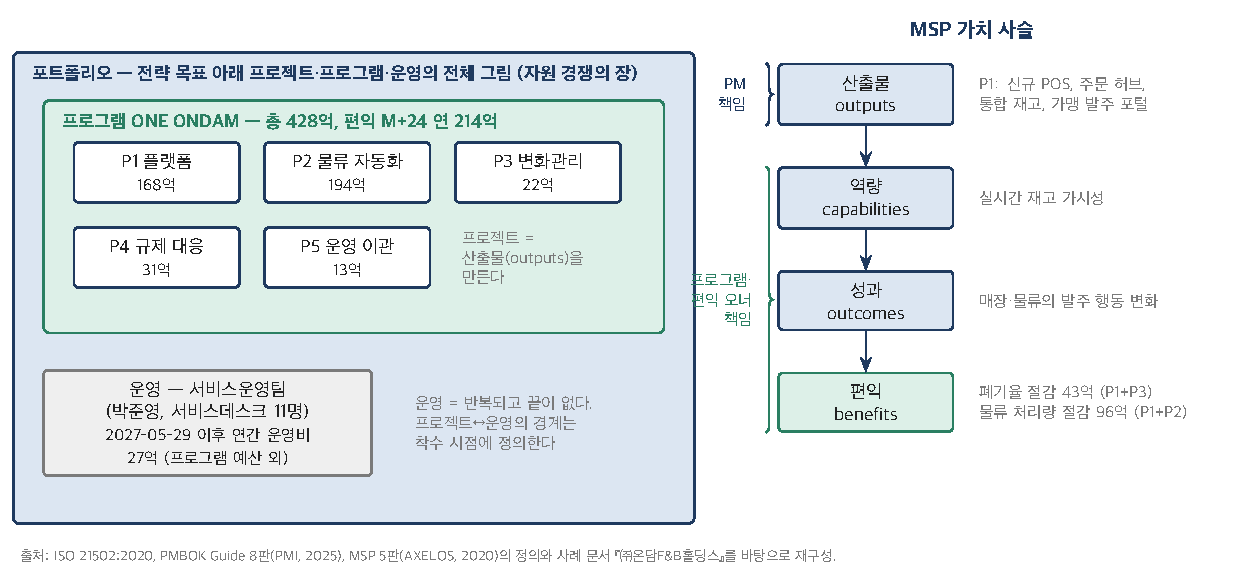
\includegraphics[width=1.00\textwidth,height=0.72\textheight,keepaspectratio]{../그림/PM_Day1/fig_1_1_hierarchy.pdf}
\par\nobreak\vspace{1pt}{\scriptsize\color{mDarkTeal!70}그림 1-1. 포트폴리오·프로그램·프로젝트·운영의 관계와 MSP 가치 사슬\par}
\end{center}
\framebreak
\begin{itemize}
\item\relax 총 428억, 다섯 프로젝트: \textbf{P1 플랫폼 168억} · P2 물류 자동화 194억 · P3 변화관리 22억 · P4 규제 대응 31억 · P5 운영 이관 13억
\item\relax 이사회 승인 편익 M+24 연간 절감 \textbf{214억} — 어느 한 프로젝트가 만들지 않는다
\par\nobreak
\begin{itemize}
\item\relax 폐기율 절감 43억 = P1의 실시간 재고(산출물) $\rightarrow$ 매장·물류의 발주 행동 변화(역량$\rightarrow$성과) $\rightarrow$ 편익
\item\relax 물류 처리량 96억 = P2 설비 + P1 재고 원장이 \textbf{함께} 작동해야 나온다
\end{itemize}
\item\relax P1의 산출물은 명확하다(POS, 주문 허브, 통합 재고, 가맹 포털, 통합 계층·데이터 전환). \textbf{P1의 편익은 P1 혼자 만들지 못한다}
\item\relax 운영과의 경계: P5 종료(2027-05-29) 이후는 서비스운영팀(박준영, 11명)의 것. 연 운영비 27억은 428억 밖
\end{itemize}
\begin{itemize}
\item\relax 두 방향의 오류 (§1.1): \textbf{프로그램을 프로젝트 도구로}("전사 혁신 과제", "DX TF" — 편익 소유자 소멸, 프로젝트 간 의존 미관리, 종료 조건 흐려짐) / \textbf{운영을 프로젝트로 포장}(연례 업그레이드에 헌장·킥오프·종료 보고서 — 반복되고 끝이 없는 일은 운영, ITIL의 영역)
\end{itemize}
\note{§1.1 "온담의 사례로 읽기"와 "실무에서 어떻게 틀리는가". 수강생 회사의 "TF"가 정의상 프로그램인지 묻는다(생각해 볼 질문 1). PMBOK 8판 첫 원칙 "총체적 관점"이 이 관계를 보라는 요구. 편익이 프로젝트 경계를 넘어 발생한다는 사실 자체가 프로그램의 존재 이유임을 강조한다. "프로젝트가 끝나는 지점과 운영이 시작되는 지점을 착수 시점에 정의하지 않으면 종료 시점에 반드시 다툼이 일어난다"를 말하고 Day4 예고. 예상 소요 8분.}
\end{frame}

% ---- md slide 8: 프로젝트는 왜 실패하는가 — "성공률 30%"를 믿으면 안 되는 이유
\begin{frame}[allowframebreaks=1.0]{프로젝트는 왜 실패하는가 — "성공률 30\%"를 믿으면 안 되는 이유}
\small
\begin{center}\usebeamercolor[fg]{normal text}
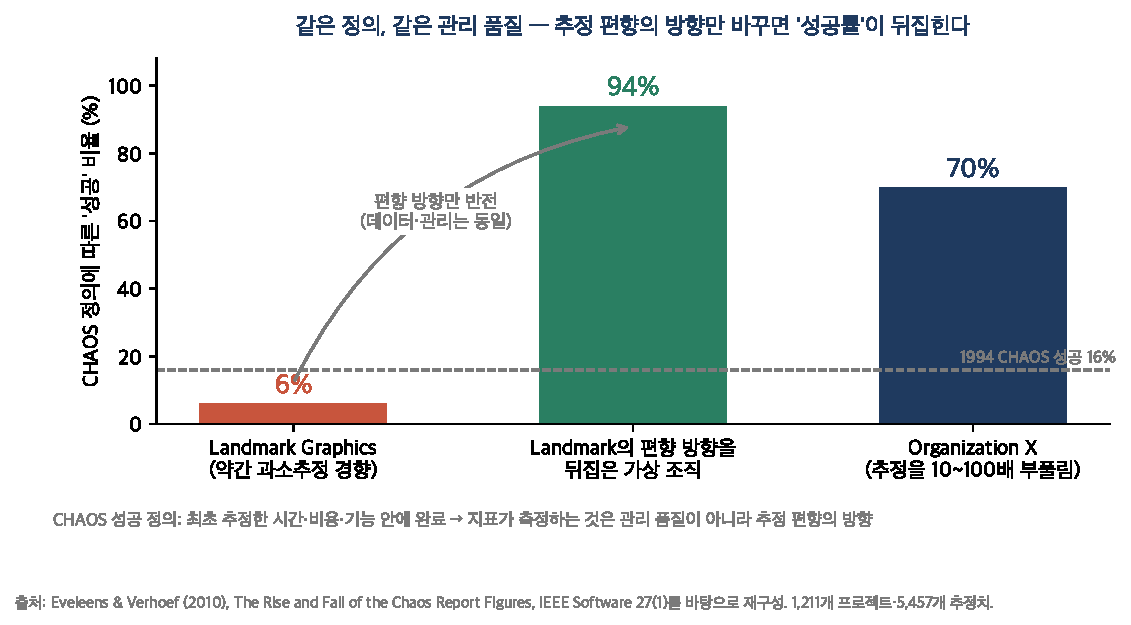
\includegraphics[width=1.00\textwidth,height=0.72\textheight,keepaspectratio]{../그림/PM_Day1/fig_1_2_chaos_bias.pdf}
\par\nobreak\vspace{1pt}{\scriptsize\color{mDarkTeal!70}그림 1-2. CHAOS 성공 정의의 결함 — 6\% / 94\% / 70\%\par}
\end{center}
\framebreak
\begin{itemize}
\item\relax Standish CHAOS Report(1994\textasciitilde{}): 성공 16\% · challenged 53\% — 30년간 업계 상식이 된 숫자
\item\relax \textbf{Eveleens \& Verhoef (2010, IEEE Software)} — 정의가 잘못되었다
\par\nobreak
\begin{itemize}
\item\relax Standish의 "성공" = 최초 추정한 시간·비용·기능 안에 완료
\item\relax 추정을 10\textasciitilde{}100배 부풀리는 조직(Organization X)은 약 \textbf{70\% 성공}, 추정이 정확하지만 약간 과소인 조직은 \textbf{6\% 성공}, 편향만 뒤집으면 \textbf{94\% 성공}
\item\relax 이 지표는 관리 품질이 아니라 \textbf{추정이 어느 방향으로 편향되어 있는가}를 측정한다
\end{itemize}
\item\relax 네 가지 문제: 오도적 / 일방적 / \textbf{추정 관행을 왜곡} / 의미 없는 숫자
\item\relax 결론은 "프로젝트는 실패하지 않는다"가 아니다 — \textbf{이 숫자로는 아무것도 알 수 없다}
\end{itemize}
\note{§1.2 "흔히 인용되는 숫자"와 "Eveleens \& Verhoef". 세 번째 문제가 실무에서 가장 중요하다 — 이 지표를 KPI로 쓰는 조직에서 합리적 행동은 추정을 부풀리는 것이다. "여러분 회사가 일정 준수율을 PM 평가 지표로 쓰고 있다면 같은 메커니즘이 이미 작동하고 있다"를 던진다(생각해 볼 질문 2). Jørgensen \& Moløkken-Østvold(2006)의 "189\% 초과" 재검토도 한 줄. 예상 소요 8분.}
\end{frame}

% ---- md slide 9: Flyvbjerg — 다른 데이터, 다른 결론
\begin{frame}[allowframebreaks=1.0]{Flyvbjerg — 다른 데이터, 다른 결론}
\small
\begin{center}\usebeamercolor[fg]{normal text}
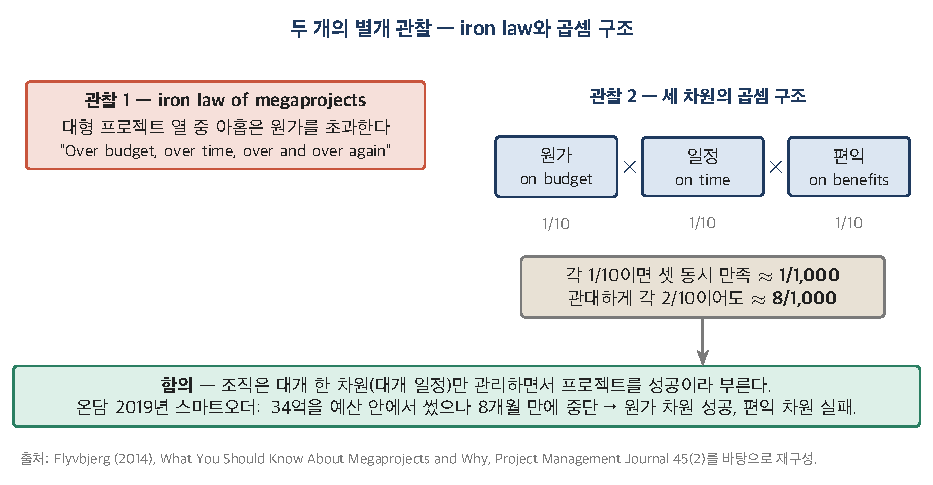
\includegraphics[width=0.48\textwidth,height=0.72\textheight,keepaspectratio]{../그림/PM_Day1/fig_1_2_flyvbjerg_multiply.pdf}
\hfill
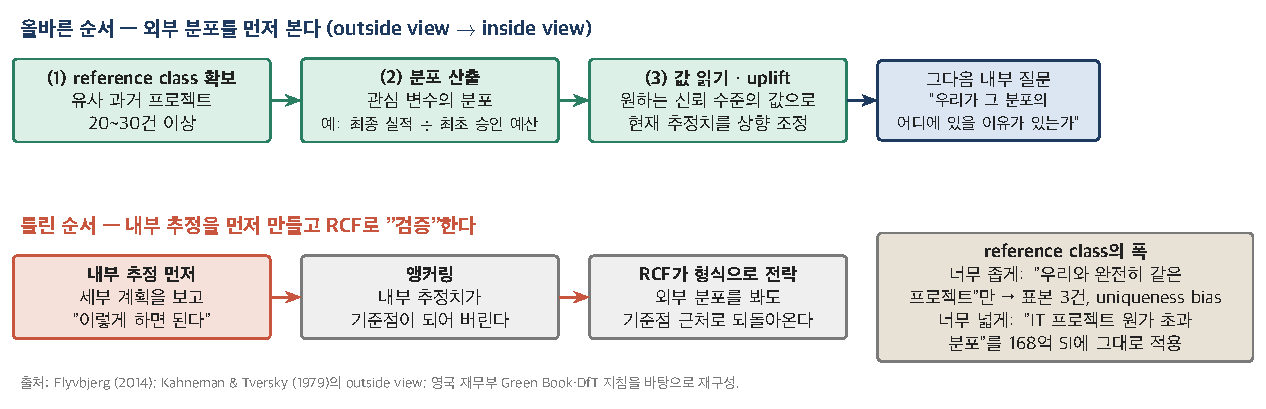
\includegraphics[width=0.48\textwidth,height=0.72\textheight,keepaspectratio]{../그림/PM_Day1/fig_1_2_rcf.pdf}
\par\nobreak\vspace{1pt}{\scriptsize\color{mDarkTeal!70}그림 1-3. iron law와 세 차원의 곱셈 구조 / 그림 1-4. RCF 3단계와 앵커링\par}
\end{center}
\framebreak
\begin{itemize}
\item\relax 응답 설문이 아니라 실제 인프라 프로젝트의 \textbf{최초 승인 예산 vs 최종 실적}을 수십 년 수집
\item\relax \textbf{Iron law of megaprojects}: "Over budget, over time, over and over again" — 열 중 아홉이 원가 초과
\item\relax 별개의 논증 — 원가·일정·편익 각 1/10이면 셋 동시 만족은 약 \textbf{1/1,000} (관대하게 2/10씩이면 8/1,000)
\par\nobreak
\begin{itemize}
\item\relax 조직은 대개 한 차원(일정)만 관리하면서 성공이라 부른다. 온담 2019 스마트오더: 34억 예산 안 $\rightarrow$ 8개월 만에 중단 (원가 성공, 편익 실패)
\end{itemize}
\item\relax 처방 — \textbf{Reference Class Forecasting (RCF)}: ① 유사 과거 프로젝트 20\textasciitilde{}30건 확보 $\rightarrow$ ② 관심 변수(실적$\div$최초 예산)의 분포 $\rightarrow$ ③ 그 분포에서 uplift 또는 상대 위험 판단
\item\relax 순서가 핵심: \textbf{외부 분포를 먼저, 내부 추정은 나중에} — 반대로 하면 앵커링. reference class를 너무 좁게 잡으면 uniqueness bias
\end{itemize}
\note{§1.2 "Flyvbjerg". iron law와 곱셈 구조는 자주 뒤섞여 인용되므로 분리해서 말한다. 영국 재무부 Green Book·DfT가 RCF를 공식 지침에 탑재했다는 사실로 "학술 논쟁이 아니라 제도"임을 보인다. IT 원가 초과가 멱함수 분포(2022 JMIS)라는 점 — 평균에 맞춘 컨틴전시가 틀린 이유 — 은 Day2·Day3 예고로 한 줄만. 예상 소요 8분.}
\end{frame}

% ---- md slide 10: 그러면 Flyvbjerg의 숫자는 믿어도 되는가 — 자기 조직의 base rate
\begin{frame}[allowframebreaks=1.0]{그러면 Flyvbjerg의 숫자는 믿어도 되는가 — 자기 조직의 base rate}
\small
\begin{itemize}
\item\relax Flyvbjerg 표본은 교통·에너지·올림픽 중심. 2022년 IT 5,392건도 특정 DB의 표본 — 168억 SI에 그대로 적용은 \textbf{reference class를 너무 넓게} 잡는 반대쪽 오류
\item\relax 배울 것은 숫자가 아니라 태도: \textbf{남의 통계를 인용하지 말고 자기 조직의 base rate를 만들라}
\item\relax 온담에 이미 있는 데이터
\end{itemize}
{\usebeamercolor[fg]{normal text}\small\setlength{\tabcolsep}{3pt}\renewcommand{\arraystretch}{1.12}
\begin{tabular}{@{}>{\raggedright\arraybackslash}p{0.161\textwidth}>{\raggedright\arraybackslash}p{0.237\textwidth}>{\raggedright\arraybackslash}p{0.161\textwidth}>{\raggedright\arraybackslash}p{0.427\textwidth}@{}}
\toprule
\textbf{연도} & \textbf{사업} & \textbf{규모} & \textbf{결과} \\
\midrule
2014 & SAP 도입 & 74억 & (계획 대비 실적 미기재 — 워크북에서 가정) \\
2019 & 스마트오더 & 34억 & \textbf{중단} (8개월) \\
2022 & WMS 고도화 & 12억 & \textbf{범위 63\% 축소} \\
2025 & 검사기록 디지털화 견적 & 34억 & 반려 \\
\bottomrule
\end{tabular}}
\par\smallskip
\begin{itemize}
\item\relax 네 건은 reference class로는 너무 적다. 그러나 "정보화 사업 4건 중 2건 중단·축소"는 P1 초기 리스크 등록부에 들어가야 할 base rate다
\end{itemize}
\begin{itemize}
\item\relax 통계 인용의 네 가지 오류 (§1.2): 임원 보고서에 CHAOS를 "업계 표준 실패율"로 인용(그 자리에서 신뢰를 잃는다) / "그러니 PM은 소용없다"는 결론 / iron law를 냉소로("best practice는 예외, average practice가 재앙"이 실제 결론) / 자기 base rate를 만들지 않음
\end{itemize}
\note{§1.2 "그러면 Flyvbjerg의 숫자는 믿어도 되는가"와 "실무에서 어떻게 틀리는가". 제안서·임원 보고서에서 CHAOS 수치를 빼라는 것이 오늘의 첫 실무 처방. 이사회 승인 조건 5항(내부감사 지적 재발 방지)이 같은 인식이라는 점을 연결한다. 워크북 §1 심화 과제(과거 4건을 reference class 출발점으로)와 6교시 프리모템의 세 번째 원천(base rate)을 예고. 예상 소요 5분.}
\end{frame}

% ---- md slide 11: 성공의 두 정의 — Cooke-Davies (2002)
\begin{frame}[allowframebreaks=1.0]{성공의 두 정의 — Cooke-Davies (2002)}
\small
\begin{center}\usebeamercolor[fg]{normal text}
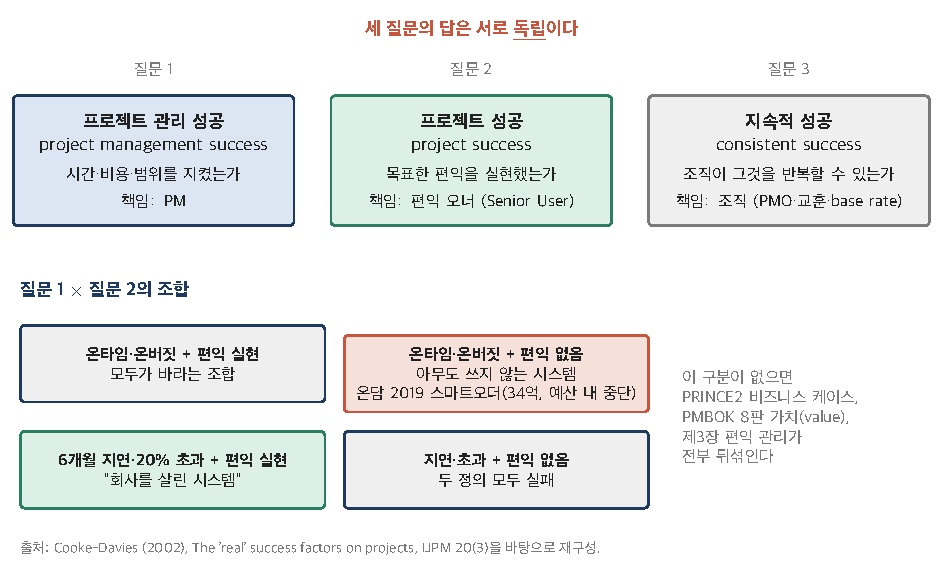
\includegraphics[width=1.00\textwidth,height=0.72\textheight,keepaspectratio]{../그림/PM_Day1/fig_1_2_cooke_davies.pdf}
\par\nobreak\vspace{1pt}{\scriptsize\color{mDarkTeal!70}그림 1-6. Cooke-Davies 성공 세 정의와 2$\times$2 조합 (스마트오더 위치)\par}
\end{center}
\framebreak
{\usebeamercolor[fg]{normal text}\footnotesize\setlength{\tabcolsep}{3pt}\renewcommand{\arraystretch}{1.12}
\begin{tabular}{@{}>{\raggedright\arraybackslash}p{0.200\textwidth}>{\raggedright\arraybackslash}p{0.346\textwidth}>{\raggedright\arraybackslash}p{0.181\textwidth}>{\raggedright\arraybackslash}p{0.258\textwidth}@{}}
\toprule
\textbf{질문} & \textbf{이름} & \textbf{판정 시점} & \textbf{온담 P1에서} \\
\midrule
시간·비용·범위를 지켰는가 & \textbf{프로젝트 관리 성공} (project management success) & 종료 시점 (G4 2027-05-29) & 156억 집행 한도, 다섯 산출물, SAC 충족 \\
목표한 편익을 실현했는가 & \textbf{프로젝트 성공} (project success) & 종료 후 (G5 2028-03-31) & 폐기율 2.2\%, 결품률 1.5\%, 리드타임 12h \\
조직이 그것을 반복할 수 있는가 & \textbf{지속적 성공} (consistent success) & 여러 프로젝트에 걸쳐 & 온담의 과거 4건 \\
\bottomrule
\end{tabular}}
\par\smallskip
\begin{itemize}
\item\relax 세 답은 \textbf{서로 독립}이다 — 온타임·온버짓인데 아무도 안 쓰는 시스템 / 6개월 지연·20\% 초과인데 회사를 살린 시스템
\item\relax 이 구분이 없으면 PRINCE2 비즈니스 케이스, PMBOK 8판의 가치, 편익 관리 논의가 전부 뒤섞인다
\end{itemize}
\note{§1.2 "성공의 두 정의". 과정 전 제출 과제("최근 종료 프로젝트의 온타임·온버짓 O/X와 편익 달성 O/X")를 여기서 꺼낸다 — 두 답이 다른 프로젝트가 있는 수강생에게 한 문장씩 말하게 한다(5분 토론). 이 구분은 헌장 항목 3(성공 기준 두 층)에서 그대로 쓰인다. 예상 소요 7분.}
\end{frame}

% ---- md slide 12: 프로젝트를 임시조직으로 본다는 것 — Lundin & Söderholm (1995)
\begin{frame}[allowframebreaks=1.0]{프로젝트를 임시조직으로 본다는 것 — Lundin \& Söderholm (1995)}
\small
\par\smallskip\noindent{\usebeamercolor[fg]{normal text}\textbf{네 가지 구조 개념 (4T)}\par}\nobreak
\begin{itemize}
\item\relax \textbf{시간(Time)} — 영구조직에서 시간은 흐르지만, 임시조직에서 시간은 \textbf{소모된다}
\item\relax \textbf{과업(Task)} — 과업이 끝나면 존재 이유가 사라진다
\item\relax \textbf{팀(Team)} — 소속감은 과업에 묶여 있고, 과업 후 흩어진다
\item\relax \textbf{전환(Transition)} — 이전 상태에서 이후 상태로 바꾸기 위해 존재한다
\end{itemize}
\par\smallskip\noindent{\usebeamercolor[fg]{normal text}\textbf{네 가지 행위 개념}\par}\nobreak
\begin{itemize}
\item\relax 행위 기반 기업가정신 — 착수는 분석의 결과가 아니라 \textbf{행위}의 결과
\item\relax 몰입 형성을 위한 단편화 — WBS는 계획 도구이기 전에 \textbf{몰입 도구}
\item\relax 계획된 고립 — 별도 사무실·예산·보고선
\item\relax 제도화된 종료 — 종료 보고서, 해산, 복귀
\end{itemize}
\framebreak
\begin{center}\usebeamercolor[fg]{normal text}
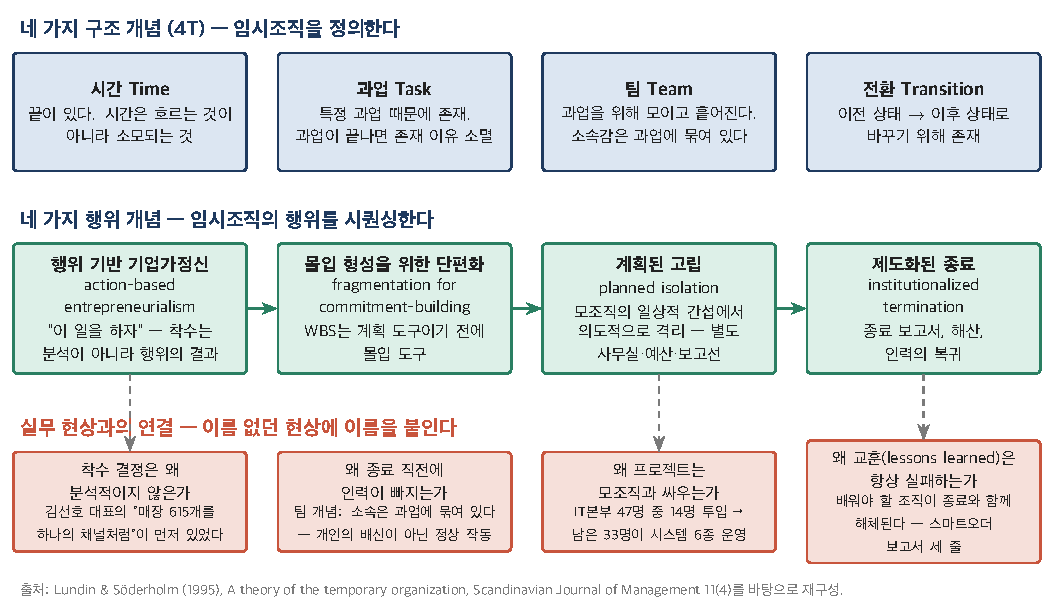
\includegraphics[width=1.00\textwidth,height=0.80\textheight,keepaspectratio]{../그림/PM_Day1/fig_1_3_temporary_org.pdf}
\par\nobreak\vspace{1pt}{\scriptsize\color{mDarkTeal!70}그림 1-7. 임시조직 이론 — 4T·4 행위 개념·실무 현상\par}
\end{center}
\note{§1.3 개념. 표준의 라이프사이클 그림이 설명하지 못하는 것 — "왜 프로젝트 안의 사람들이 그렇게 행동하는가" — 을 설명하는 렌즈라고 소개한다. 흔한 오류: "임시조직"을 "한시적 조직"이라는 사전적 의미로만 쓰는 것, 4T를 헌장 체크리스트로 만드는 것. 예상 소요 6분.}
\end{frame}

% ---- md slide 13: 이 렌즈가 설명하는 네 가지 현상 + "어떤 프로젝트도 섬이 아니다"
\begin{frame}[allowframebreaks=1.0]{이 렌즈가 설명하는 네 가지 현상 + "어떤 프로젝트도 섬이 아니다"}
\small
{\usebeamercolor[fg]{normal text}\footnotesize\setlength{\tabcolsep}{3pt}\renewcommand{\arraystretch}{1.12}
\begin{tabular}{@{}>{\raggedright\arraybackslash}p{0.276\textwidth}>{\raggedright\arraybackslash}p{0.313\textwidth}>{\raggedright\arraybackslash}p{0.396\textwidth}@{}}
\toprule
\textbf{실무자가 매일 겪는 것} & \textbf{설명하는 개념} & \textbf{온담에서} \\
\midrule
교훈(lessons learned)은 왜 항상 실패하는가 & 제도화된 종료 — 배울 조직이 종료와 함께 해체 & 스마트오더 종료 보고서 중단 사유 세 줄 \\
종료 직전에 왜 인력이 빠지는가 & 팀 — 과업의 끝이 보이면 다음 과업을 찾는 것이 정상 & 안정화 기간의 핵심 개발자 이탈 \\
프로젝트는 왜 모조직과 싸우는가 & 계획된 고립 — 프로젝트의 고립은 운영의 부담 & IT본부 47명 중 14명 투입, 33명이 시스템 6종·인터페이스 47본 운영 \\
착수 결정은 왜 분석적이지 않은가 & 행위 기반 기업가정신 & "매장 615개를 하나의 채널처럼"이 먼저, 비즈니스 케이스는 나중 \\
\bottomrule
\end{tabular}}
\par\smallskip
\begin{itemize}
\item\relax \textbf{Engwall (2003)}: 일정·예산·조직 구성·핵심 갈등은 착수 전에 조직의 역사와 정치로 이미 결정되어 있다 $\rightarrow$ 킥오프 시점 PM의 진짜 일은 \textbf{이미 결정된 것들을 목록화하는 것}
\par\nobreak
\begin{itemize}
\item\relax 컷오버 2027-02 = 2019 사모펀드 계약의 IPO 조항 / 인터페이스 우선 = 2011 OD-POS를 박세연이 직접 만듦 / 가맹 경계 = 2019 스마트오더 중단 경험
\end{itemize}
\item\relax 처방: 새 프로젝트 첫 주에 \textbf{직전 프로젝트 두세 개의 종료 보고서를 읽어라}
\end{itemize}
\note{§1.3 "왜 유용한가"와 "어떤 프로젝트도 섬이 아니다". Engwall은 "맥락이 중요하다"는 상투구가 아니라 인과 주장임을 강조 — 직전 프로젝트의 정치적 결과가 이번 프로젝트의 특징을 설명한다. 종료 이후 경로(P5, 다음 배치)를 착수 시점에 설계해야 인력 이탈을 막는다는 처방도 한 줄. 생각해 볼 질문 4(착수 전 결정된 비율). 예상 소요 9분.}
\end{frame}

% ---- md slide 14: 프로젝트 유형은 하나가 아니다 — NTCP 다이아몬드 (Shenhar & Dvir, 2007)
\begin{frame}[allowframebreaks=1.0]{프로젝트 유형은 하나가 아니다 — NTCP 다이아몬드 (Shenhar \& Dvir, 2007)}
\small
{\usebeamercolor[fg]{normal text}\footnotesize\setlength{\tabcolsep}{3pt}\renewcommand{\arraystretch}{1.12}
\begin{tabular}{@{}>{\raggedright\arraybackslash}p{0.123\textwidth}>{\raggedright\arraybackslash}p{0.195\textwidth}>{\raggedright\arraybackslash}p{0.391\textwidth}>{\raggedright\arraybackslash}p{0.276\textwidth}@{}}
\toprule
\textbf{축} & \textbf{질문} & \textbf{단계} & \textbf{이 축이 결정하는 것} \\
\midrule
\textbf{Novelty} & 시장·사용자에게 얼마나 새로운가 & derivative / platform / breakthrough (\textbf{3}) & 요구사항 확정 시점, 시장 조사 신뢰도 \\
\textbf{Technology} & 기술이 얼마나 성숙한가 & low / medium / high / super-high (\textbf{4}) & 설계 동결 시점, 설계 반복 횟수 \\
\textbf{Complexity} & 범위·계층이 얼마나 넓은가 & assembly / system / array (\textbf{3}) & 조직·절차의 형식성, 하도급·인터페이스 관리 \\
\textbf{Pace} & 시간이 얼마나 결정적인가 & regular / fast-competitive / time-critical / blitz (\textbf{4}) & 의사결정 위임 수준, 상위 관리자 개입 \\
\bottomrule
\end{tabular}}
\par\smallskip
\begin{itemize}
\item\relax 네 축은 \textbf{직교}한다 — 합산해 "난이도 3.2등급"을 만드는 순간 모델은 무의미해진다
\item\relax 다이아몬드가 바깥쪽일수록 리스크가 크고 관리는 더 유연해야 한다. 축마다 \textbf{다른 처방}
\end{itemize}
\note{§1.4 개념. 단계 수 3/4/3/4를 정확히 — 교재 오류가 자주 나는 지점이다. PMBOK 7·8이 테일러링을 강조하면서 판단 기준을 주지 않는 공백을 이 모델이 메운다고 위치시킨다. 예상 소요 5분.}
\end{frame}

% ---- md slide 15: 온담 P1을 NTCP로 진단하면 — "표준 SI 프로젝트"가 아니다
\begin{frame}[allowframebreaks=1.0]{온담 P1을 NTCP로 진단하면 — "표준 SI 프로젝트"가 아니다}
\small
\begin{center}\usebeamercolor[fg]{normal text}
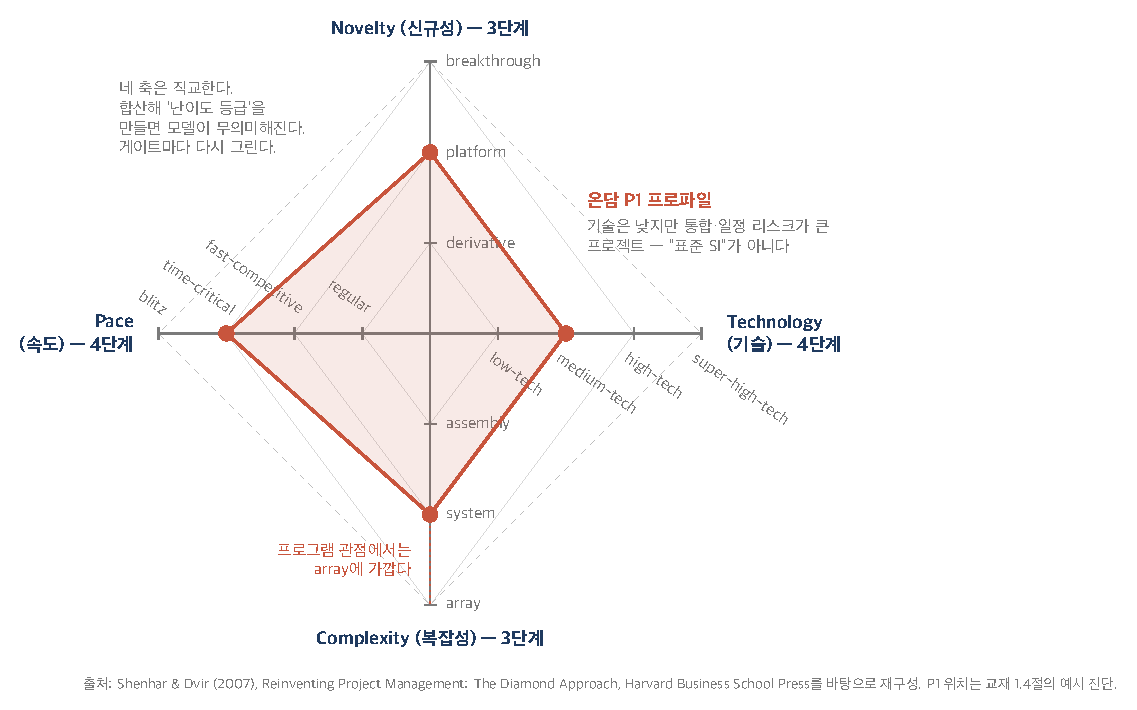
\includegraphics[width=1.00\textwidth,height=0.72\textheight,keepaspectratio]{../그림/PM_Day1/fig_1_4_ntcp.pdf}
\par\nobreak\vspace{1pt}{\scriptsize\color{mDarkTeal!70}그림 1-8. NTCP 다이아몬드 — 온담 P1의 위치 (3/4/3/4)\par}
\end{center}
\framebreak
\begin{itemize}
\item\relax \textbf{Novelty = platform} — 옴니채널·클라우드 POS는 시장에 흔하지만, 온담 사용자(매장 1,510명·가맹 331명·B2B 260개사)에게는 업무 방식이 바뀌는 플랫폼급. 로컬 DB+야간 동기화 $\rightarrow$ 중앙 실시간이므로 derivative 아님 $\rightarrow$ 처방: 요구사항은 초기에 대부분 확정 가능하되 사용자 검증 여러 번 (스프린트 36회와 정합)
\item\relax \textbf{Technology = medium} — 클라우드·API GW·MDM·SAP 애드온은 성숙. 그러나 문서 없는 인터페이스 13본, 1,842 테이블·7.4TB, 3PL WMS라는 \textbf{기존 기술의 미지}가 크다 $\rightarrow$ 설계 동결 1\textasciitilde{}2회 (설계 스프린트 6회, 전환 리허설 3회)
\item\relax \textbf{Complexity = array에 가까운 system} — P1 자체는 system, 프로그램 관점(P2·P4·P5 인터페이스, 벤더 11개사, 별도 법인, 3PL)에서는 array $\rightarrow$ 형식적 계약·문서·인터페이스 관리, 별도 통합 조직 (프로그램 PMO 4 + P1 PMO 3)
\item\relax \textbf{Pace = time-critical} — 컷오버 2027-02-26\textasciitilde{}28은 IPO 역산, 규제 2026-09-11·2027-03-31은 협상 불가 $\rightarrow$ 일정 최우선, 권한 위임, 상위 관리자 밀착. 대표("더 앞당기라")와 CFO("148억으로")가 이 축에서 정면 충돌 $\rightarrow$ \textbf{헌장 우선순위 항목}이 적어야 한다
\item\relax 결론: 기술은 낮지만 복잡성 array급·속도 time-critical $\rightarrow$ \textbf{기술 리스크보다 통합·일정 리스크에 자원 집중}. 같은 프로그램의 P2는 전혀 다른 프로파일
\end{itemize}
\note{§1.4 "온담 P1을 이 모델로 진단하면". 이 판단은 예시이며 워크북에서 수강생이 다시 판단한다고 말한다. 오류 셋: 합산, 착수 때 한 번만 그림(Pace는 중간에 승격), 그림만 그리고 처방을 안 정함 — 처방 규칙표가 2교시 TDR이다. 생각해 볼 질문 5(system vs array). 예상 소요 10분.}
\end{frame}

% ---- md slide 16: 분야별 대조 — 같은 단어, 다른 리듬, 다른 되돌림 비용
\begin{frame}[allowframebreaks=1.0]{분야별 대조 — 같은 단어, 다른 리듬, 다른 되돌림 비용}
\small
\begin{center}\usebeamercolor[fg]{normal text}
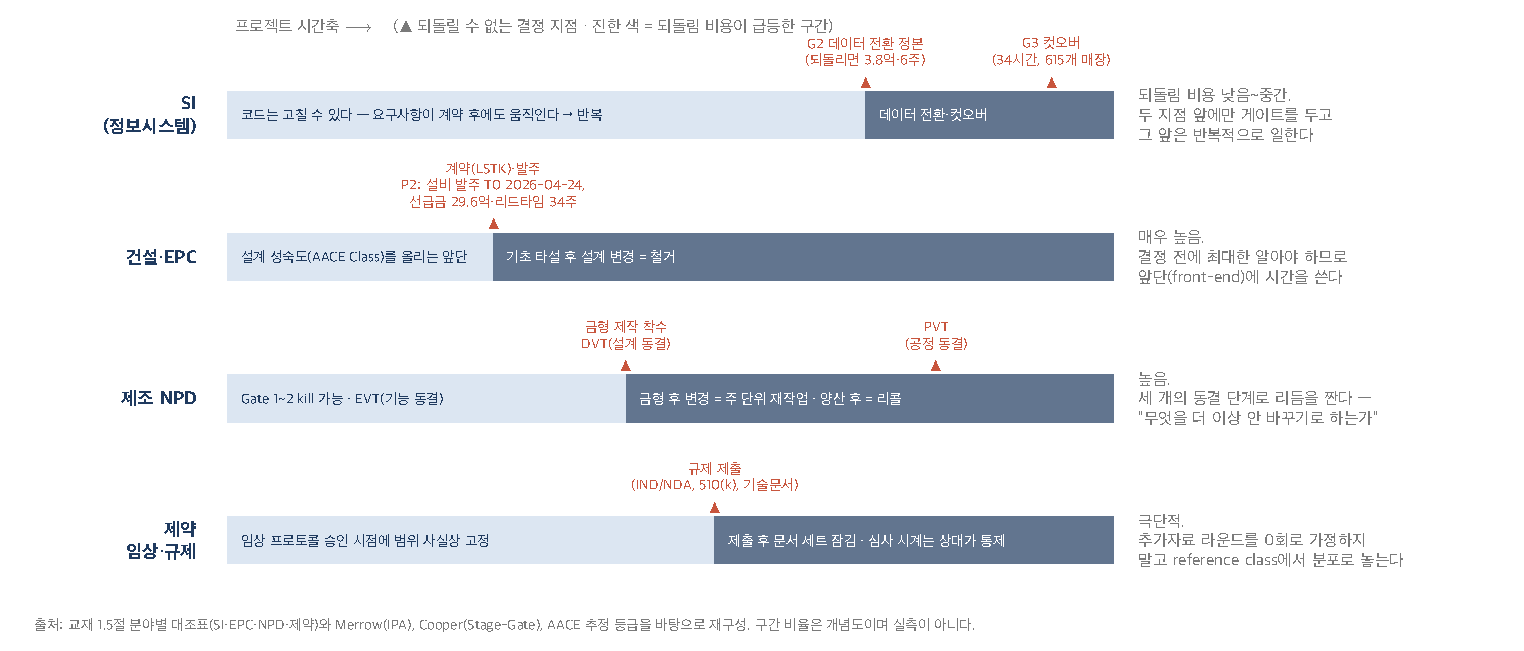
\includegraphics[width=1.00\textwidth,height=0.72\textheight,keepaspectratio]{../그림/PM_Day1/fig_1_5_reversal_cost.pdf}
\par\nobreak\vspace{1pt}{\scriptsize\color{mDarkTeal!70}그림 1-9. 분야별 되돌림 비용 시간축 대조 (SI·EPC·NPD·제약)\par}
\end{center}
\framebreak
{\usebeamercolor[fg]{normal text}\scriptsize\setlength{\tabcolsep}{3pt}\renewcommand{\arraystretch}{1.12}
\begin{tabular}{@{}>{\raggedright\arraybackslash}p{0.079\textwidth}>{\raggedright\arraybackslash}p{0.205\textwidth}>{\raggedright\arraybackslash}p{0.242\textwidth}>{\raggedright\arraybackslash}p{0.231\textwidth}>{\raggedright\arraybackslash}p{0.228\textwidth}@{}}
\toprule
\textbf{축} & \textbf{SI} & \textbf{건설·EPC} & \textbf{제조 NPD} & \textbf{제약 임상·규제} \\
\midrule
산출물 & 소프트웨어 — 수정 가능 & 물리 구조물 & 물리 제품 + 양산 공정 & \textbf{승인} — 규제기관의 결정 \\
\textbf{되돌림 비용} & 낮음\textasciitilde{}중간 (데이터 전환·컷오버는 예외) & 매우 높음 — 기초 타설 후 변경은 철거 & 높음 — 금형 후 주 단위 재작업, 양산 후 리콜 & 극단적 — 제출 후 문서 잠김, 시계는 상대가 통제 \\
리듬을 정하는 것 & 요구사항 확정, 인터페이스 상대의 준비 & 자재 리드타임, 공정 순서, 인허가 & 금형·부품 리드타임, EVT/DVT/PVT & 심사 일정, 추가자료 왕복 횟수 \\
범위 확정 시점 & 늦다 — 계약 후에도 움직임 & 이르다 — 설계 성숙도(AACE Class)가 계약 유형 결정 & 게이트마다 단계적, Gate 1\textasciitilde{}2에서 kill & 프로토콜 승인 시 사실상 고정 \\
주된 실패 & 요구 팽창, 데이터 전환, 인터페이스 미확정 & 설계 미성숙 상태의 LSTK, 동시지연 클레임 & 이빨 없는 게이트(kill 0건), 금형 뒤 설계 변경 & 추가자료 0회 가정 위의 출시일 공표 \\
\bottomrule
\end{tabular}}
\par\smallskip
\begin{itemize}
\item\relax 가장 중요한 열은 \textbf{되돌림 비용} — 되돌릴 수 있으면 실험하고 반복한다. 되돌릴 수 없으면 결정 전에 최대한 알아야 하므로 \textbf{앞단(front-end)에 시간을 쓴다}
\end{itemize}
\note{§1.5 표. SI의 되돌릴 수 없는 두 지점(데이터 전환 정본 610테이블 재매핑 3.8억·6주 / 컷오버 34시간 615매장 펌웨어) 앞에 G2·G3 게이트가 있는 이유를 말한다. 분야를 옮긴 PM의 실수 — 건설 자원 평준화·EVM CPI를 IT에 그대로, SI의 "일단 만들고 고치자"를 설비에 그대로(선급금 29.6억). 이 표가 2교시 테일러링의 토대다. 예상 소요 8분.}
\end{frame}

% ---- md slide 17: 1교시 핵심 정리
\begin{frame}[allowframebreaks=1.0]{1교시 핵심 정리}
\small
\begin{enumerate}
\item\relax 프로젝트는 \textbf{산출물}을 만들고, 프로그램은 산출물이 역량·성과를 거쳐 \textbf{편익}이 되도록 함께 관리한다. 편익이 프로젝트 경계를 넘는다는 사실이 프로그램의 존재 이유다
\item\relax CHAOS 성공률은 프로젝트 성과가 아니라 \textbf{추정 편향의 방향}을 측정한다. KPI로 쓰면 추정을 부풀리는 것이 최적 행동이 된다
\item\relax Flyvbjerg의 iron law와 3차원 곱셈은 별개. 처방은 RCF — \textbf{외부 분포 먼저, 내부 추정 나중}
\item\relax 프로젝트 관리 성공(시간·비용·범위)과 프로젝트 성공(편익)은 \textbf{독립}이다
\item\relax 임시조직론(4T + 4행위)이 교훈의 실패·종료 직전 이탈·모조직과의 긴장을 설명한다. 어떤 프로젝트도 섬이 아니다 — 착수의 진짜 일은 \textbf{이미 결정된 것의 목록화}
\item\relax NTCP(3/4/3/4)는 축별로 다른 처방. 합산하지 말고 게이트마다 다시 그린다
\item\relax 분야 차이의 핵심 변수는 \textbf{되돌림 비용}
\end{enumerate}
\note{제1장 핵심 정리 그대로. 워크북 연결 — 이 장은 워크북 §1 비즈니스 케이스 요약의 "전략적 배경"과 심화 과제(과거 4건 base rate)에 쓰인다. 쉬는 시간 전에 "여러분 회사에서 프로젝트라 불리지만 정의상 프로그램이거나 운영인 것"을 하나씩 떠올려 오게 한다. 예상 소요 4분.}
\end{frame}

\section{2교시 (90분) — 표준의 지형: 무엇을 따를 것인가}

% ---- md slide 18: 이 교시에서 배우는 것
\begin{frame}[allowframebreaks=1.0]{이 교시에서 배우는 것}
\small
\begin{itemize}
\item\relax PMBOK의 계보 — 6판, 7판, 그리고 8판의 부분 회귀 [§2.1]
\item\relax PMBOK 8판의 6 원칙과 7 성과영역 [§2.2]
\item\relax PRINCE2 7 — 프로젝트 보드, 예외 관리, 산출물 기반 계획 [§2.3]
\item\relax ISO 21502:2020 — 계약서가 인용하는 표준 [§2.4]
\item\relax 애자일·SAFe·하이브리드의 위치 [§2.5]
\item\relax 테일러링 — 되돌림 비용, Boehm-Turner, Cynefin, TDR [§2.6]
\item\relax 자격 체계의 실효성 [§2.7]
\end{itemize}
\note{제2장 전체. 시간 배분: §2.1 20분, §2.2 12분, §2.3 15분, §2.4 7분, §2.5 8분, §2.6 20분, §2.7 5분, 정리 3분. PMP 보유자는 §2.1에서 자기가 공부한 판본이 현행과 어떻게 다른지 확인하게 된다고 예고. 이 교시의 실무 산출물은 재매핑 대장과 TDR이다. 예상 소요 2분.}
\end{frame}

% ---- md slide 19: 왜 계보를 알아야 하는가 — PMBOK은 참고서인데
\begin{frame}[allowframebreaks=1.0]{왜 계보를 알아야 하는가 — PMBOK은 참고서인데}
\small
\begin{itemize}
\item\relax PMBOK Guide는 법도 계약 조건도 아니다. 그런데도 판본을 알아야 하는 이유 셋:
\par\nobreak
\begin{enumerate}
\item\relax 사내 PMO 표준·산출물 양식·직무기술서가 인용하는 \textbf{조항 번호}가 살아 있는지 죽어 있는지
\item\relax 계약서·RFP의 "PMBOK 준거" 문구 — 판본과 문서를 특정하지 않으면 \textbf{분쟁의 씨앗}
\item\relax 표준을 만드는 조직이 5년 사이에 자기 구조를 \textbf{두 번 뒤집었다}는 사실 자체가 이 분야의 현재 상태
\end{enumerate}
\end{itemize}
\begin{center}\usebeamercolor[fg]{normal text}
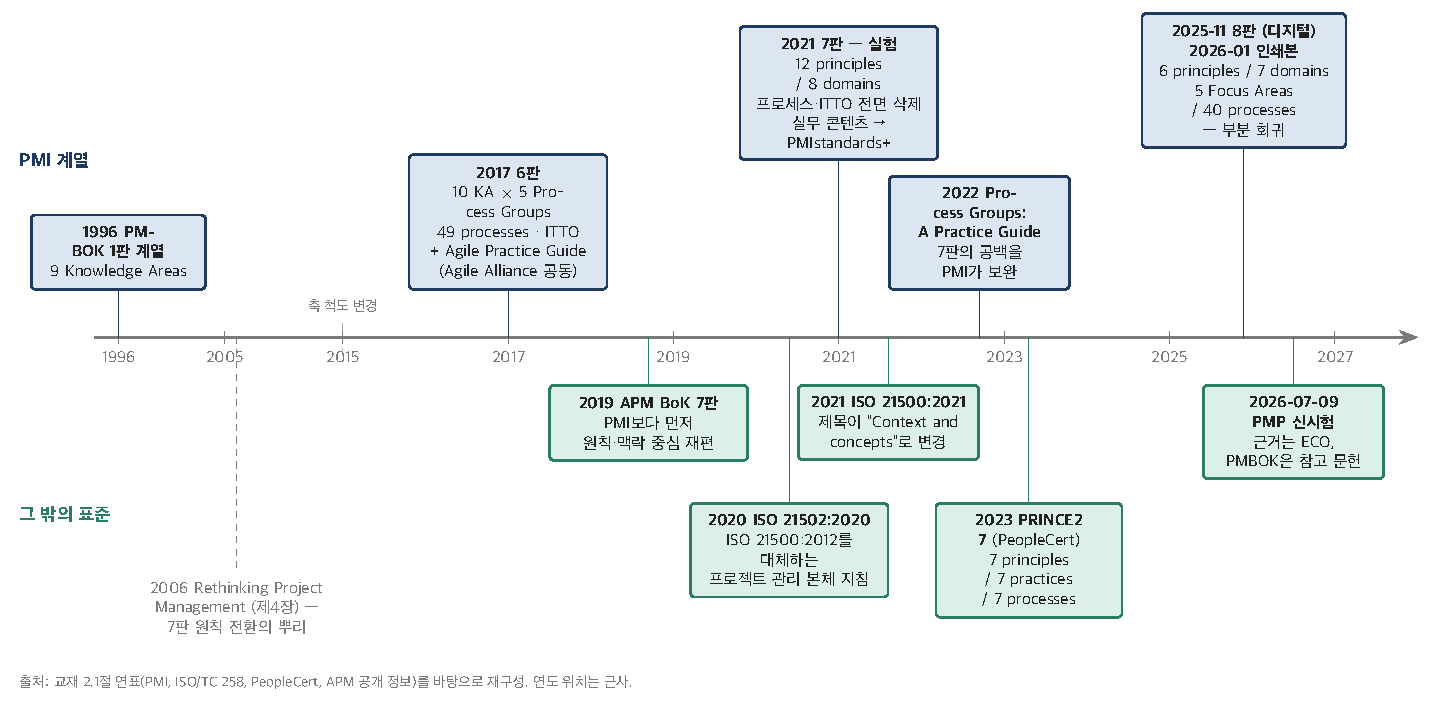
\includegraphics[width=1.00\textwidth,height=0.56\textheight,keepaspectratio]{../그림/PM_Day1/fig_2_1_pmbok_timeline.pdf}
\par\nobreak\vspace{1pt}{\scriptsize\color{mDarkTeal!70}그림 2-1. PMBOK 계보와 주변 표준 연표 1996–2026 (비선형 축)\par}
\end{center}
\note{§2.1 "왜 계보를 알아야 하는가"와 연표. 연표를 읽어 주되 2021$\rightarrow$2022$\rightarrow$2025의 세 줄(삭제 $\rightarrow$ 보완 별책 $\rightarrow$ 회귀)을 하나의 이야기로 묶는다. APM BoK 7판이 먼저였고 뿌리가 2006 Rethinking PM(마무리 §4.1)까지 올라간다는 점을 예고. 예상 소요 6분.}
\end{frame}

% ---- md slide 20: 6판 (2017) — 아직 살아 있는 사내 표준의 원본
\begin{frame}[allowframebreaks=1.0]{6판 (2017) — 아직 살아 있는 사내 표준의 원본}
\small
\begin{itemize}
\item\relax 10 지식영역 $\times$ 5 프로세스 그룹 = \textbf{49 프로세스}, 각각 ITTO(Inputs / Tools \& Techniques / Outputs)
\par\nobreak
\begin{itemize}
\item\relax 예: 4.1 Develop Project Charter — 입력: 비즈니스 문서(비즈니스 케이스·편익 관리 계획), 협약, EEF, OPA / 출력: 헌장, 가정 기록부
\end{itemize}
\item\relax 한국 기업에 깊이 뿌리내린 이유 둘
\par\nobreak
\begin{itemize}
\item\relax \textbf{감사 가능성} — 사내 감사·외부 감리·발주처 검수는 "이 문서가 있는가 없는가"를 판정할 문장을 요구한다. 49개 프로세스의 출력물 목록이 정확히 그것
\item\relax \textbf{양식이 자산} — 수년간 축적된 산출물 서식은 조직의 자산이고, 원칙 12개로는 서식이 나오지 않는다
\end{itemize}
\item\relax 이 교재는 6판을 "폐기된 판"으로 다루지 않는다 — 6판은 \textbf{한국 기업 문서체계의 원본(source document)}
\item\relax 8판이 40개 프로세스를 되살린 것은 6판이 옳았다는 뜻이 아니라 \textbf{프로세스 없는 표준은 조직이 쓸 수 없다}는 실무 피드백의 결과
\end{itemize}
\note{§2.1 "6판". 2026년 현재도 한국 대기업·공공 PMO 사내 표준은 대부분 6판 ITTO가 뼈대라는 현실을 정상 상태로 말한다. 수강생에게 "여러분 회사 표준 문서가 인용하는 판본은?"을 묻는다. 예상 소요 5분.}
\end{frame}

% ---- md slide 21: 7판 (2021) 실험 → 8판 (2025) 부분 회귀
\begin{frame}[allowframebreaks=1.0]{7판 (2021) 실험 $\rightarrow$ 8판 (2025) 부분 회귀}
\small
\begin{center}\usebeamercolor[fg]{normal text}
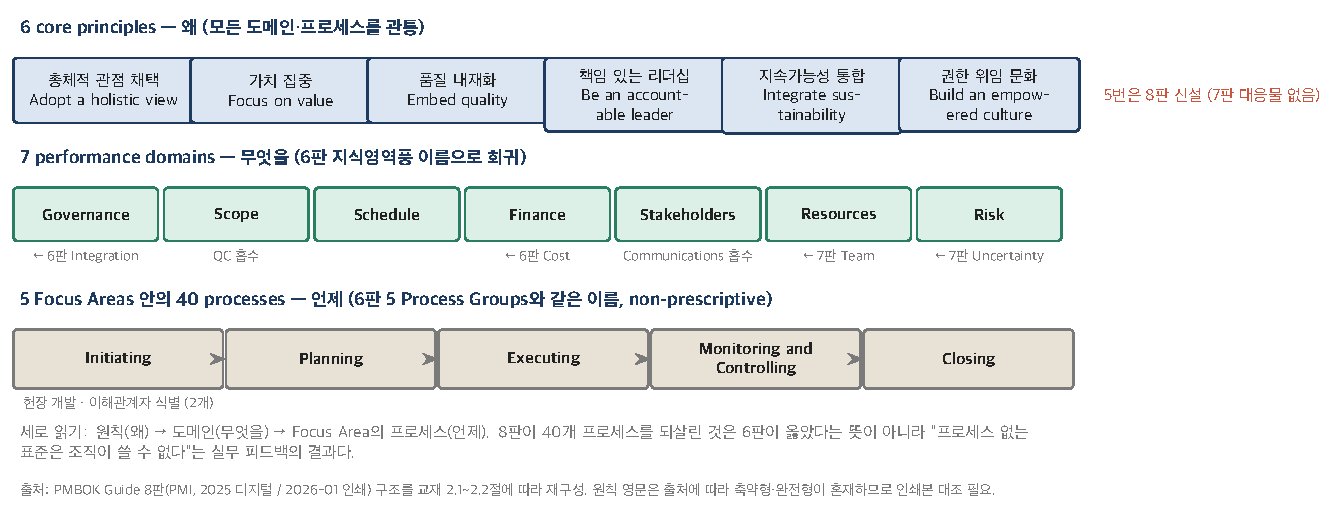
\includegraphics[width=1.00\textwidth,height=0.72\textheight,keepaspectratio]{../그림/PM_Day1/fig_2_2_pmbok8_structure.pdf}
\par\nobreak\vspace{1pt}{\scriptsize\color{mDarkTeal!70}그림 2-2. PMBOK 8판 구조 — 6 원칙 / 7 도메인 / 5 Focus Areas·40 프로세스\par}
\end{center}
\framebreak
\par\smallskip\noindent{\usebeamercolor[fg]{normal text}\textbf{7판} — 12 원칙 / 8 성과영역, 프로세스·ITTO 전부 삭제\par}\nobreak
\begin{itemize}
\item\relax 두 문서가 한 권 (ANSI 표준 『The Standard for PM』 + 『PMBOK Guide』) $\rightarrow$ "7판 준거"는 어느 문서인지 불명확
\item\relax 원칙 12개는 \textbf{감사할 수 없는 문장} ("성실하고 존중하며 배려하는 관리자가 되라"를 참/거짓으로 판정할 수 없다) $\rightarrow$ ISO 9001·CMMI·감리·위임전결 어디와도 연결 안 됨
\item\relax 실무 콘텐츠는 PMIstandards+(구독형)로 이전 — 비회원 직원은 접근 불가
\end{itemize}
\par\smallskip\noindent{\usebeamercolor[fg]{normal text}\textbf{8판} — 6 원칙 + 7 성과영역 + \textbf{5 Focus Areas 안의 40 프로세스} (non-prescriptive, 예측형·애자일·하이브리드 모두)\par}\nobreak
\begin{itemize}
\item\relax Focus Areas 이름 = Initiating / Planning / Executing / Monitoring \& Controlling / Closing — \textbf{6판의 5 Process Groups가 이름을 바꿔 돌아왔다}
\item\relax 실질 변경: \textbf{Integration $\rightarrow$ Governance}, \textbf{Cost $\rightarrow$ Finance}. Quality는 QA$\rightarrow$Governance / QC$\rightarrow$Scope로 분산, Communications는 Stakeholders에 흡수, Procurement도 독립 도메인 아님
\end{itemize}
\note{§2.1 "7판"과 "8판". 7판이 PMI의 독창이 아니라 학술 논쟁의 20년 늦은 반영이었고 8판은 그것이 실무와 충돌한 뒤의 재타협이라는 서사. 온담 CFO의 "1차연도 148억, 자산 지출 일부를 리스·운영비로" 요구가 Cost가 아니라 \textbf{Finance}의 질문이라는 예시. Quality·Communications·Procurement의 정확한 배치는 인쇄본으로 확인하라고 단서. 예상 소요 8분.}
\end{frame}

% ---- md slide 22: 한국 사내 표준은 6판에 머물러 있다 — 그 함의와 처방
\begin{frame}[allowframebreaks=1.0]{한국 사내 표준은 6판에 머물러 있다 — 그 함의와 처방}
\small
\begin{center}\usebeamercolor[fg]{normal text}
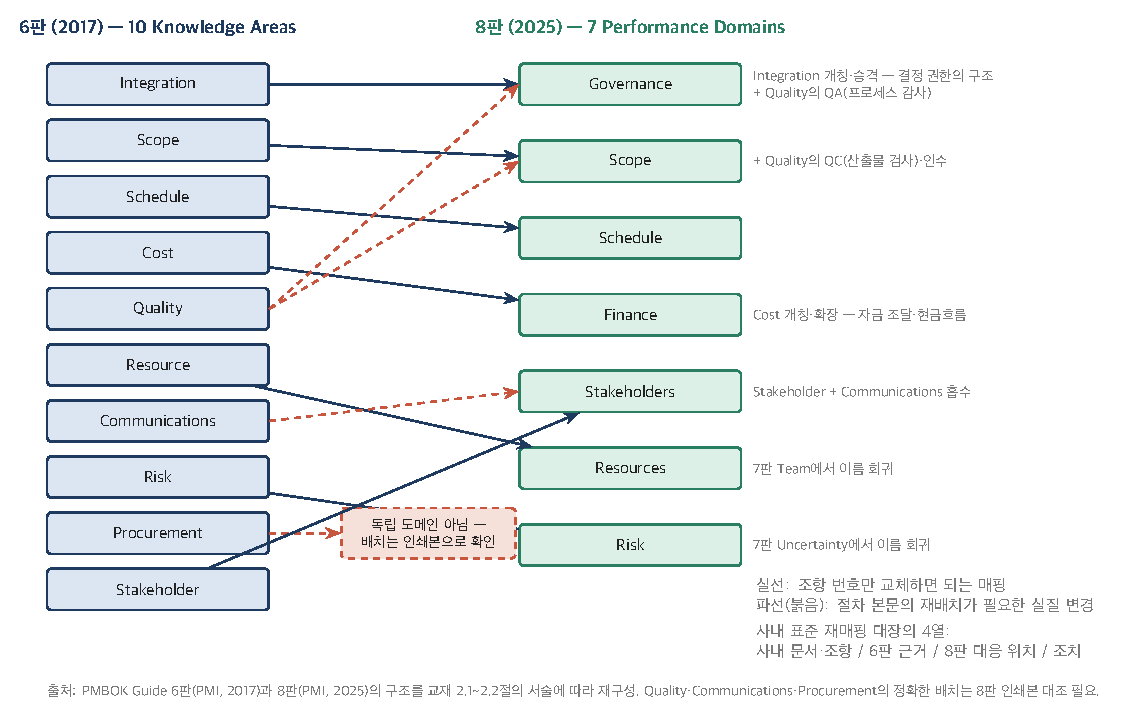
\includegraphics[width=1.00\textwidth,height=0.72\textheight,keepaspectratio]{../그림/PM_Day1/fig_2_2_domain_mapping.pdf}
\par\nobreak\vspace{1pt}{\scriptsize\color{mDarkTeal!70}그림 2-3. 6판 10 KA $\rightarrow$ 8판 7 도메인 재매핑 (실선/파선)\par}
\end{center}
\framebreak
\begin{itemize}
\item\relax 여러분 다수는 \textbf{두 판본 뒤처진 사내 표준}으로 일하면서 \textbf{한 판본 뒤처진 자격 지식}을 갖고 있다. 부끄러운 일이 아니라 정상 상태
\item\relax 함의 ①: "PMBOK 6판 4.6 Perform Integrated Change Control" 같은 조항 번호는 현행에 없다 $\rightarrow$ 외부 감리·발주처가 "현행 표준 준거"를 요구하면 방어 불가
\item\relax 처방은 재작성이 아니라 \textbf{재매핑 대장} 네 열
\end{itemize}
{\usebeamercolor[fg]{normal text}\small\setlength{\tabcolsep}{3pt}\renewcommand{\arraystretch}{1.12}
\begin{tabular}{@{}>{\raggedright\arraybackslash}p{0.194\textwidth}>{\raggedright\arraybackslash}p{0.132\textwidth}>{\raggedright\arraybackslash}p{0.254\textwidth}>{\raggedright\arraybackslash}p{0.405\textwidth}@{}}
\toprule
\textbf{사내 문서·조항} & \textbf{6판 근거} & \textbf{8판 대응 위치} & \textbf{조치} \\
\midrule
통합변경통제 절차서 & 4.6 & Governance 도메인 & 조항 번호만 교체, 절차 본문 유지 \\
원가관리계획서 & 7.1 & Finance 도메인 & 명칭 변경, 자금 조달·현금흐름 항목 신설 검토 \\
품질보증 절차서 & 8.x & QA$\rightarrow$Governance / QC$\rightarrow$Scope & 조직마다 결정 필요 \\
\bottomrule
\end{tabular}}
\par\smallskip
\begin{itemize}
\item\relax 함의 ②: PMP를 승진 요건으로 건 회사는 시험 개정 전후 형평 문제 (인사의 문제이지만 PM이 먼저 알아야)
\item\relax 함의 ③ (가장 중요): \textbf{판본이 바뀌어도 살아남는 산출물} — 헌장, 범위·일정·원가 기준선, 리스크 등록부, 변경 기록, 이해관계자 등록부. 이 소수를 중심으로 사내 표준을 다시 보는 것이 Day4 과제
\end{itemize}
\note{§2.1 "한국 기업 사내 표준이 6판에 머물러 있다는 현실"과 "실무에서 어떻게 틀리는가". 오류 사례: 7판이 나왔다고 프로세스·산출물 목록을 지운 조직이 6개월 뒤 감사에서 "판정 기준 없음" 지적으로 원복. "8판이 테일러링 원칙을 버렸다"도 오류 — 7판 \#7이 8판에서는 각 도메인 안에 분산 배치. 생각해 볼 질문 1. 예상 소요 6분.}
\end{frame}

% ---- md slide 23: PMBOK 8판의 6 core principles
\begin{frame}[allowframebreaks=1.0]{PMBOK 8판의 6 core principles}
\small
{\usebeamercolor[fg]{normal text}\footnotesize\setlength{\tabcolsep}{3pt}\renewcommand{\arraystretch}{1.12}
\begin{tabular}{@{}>{\raggedright\arraybackslash}p{0.071\textwidth}>{\raggedright\arraybackslash}p{0.259\textwidth}>{\raggedright\arraybackslash}p{0.196\textwidth}>{\raggedright\arraybackslash}p{0.459\textwidth}@{}}
\toprule
\textbf{\#} & \textbf{원칙} & \textbf{7판에서} & \textbf{온담에서 보이는 모습} \\
\midrule
1 & \textbf{총체적 관점 채택} (Adopt a holistic view) & \#5 시스템 상호작용 + \#9 복잡성 흡수 & "P2가 늦으면 P1 컷오버가 밀린다"를 리스크 등록부에 적는 것 \\
2 & \textbf{가치 집중} (Focus on value) & \#4 유지 + \#3·\#11·\#12 흡수 & 편익 214억 산출 근거를 항목별로 요구하는 CFO의 질문은 PM의 적이 아니라 이 원칙의 실행 \\
3 & \textbf{품질 내재화} (Embed quality) & \#8 "Build" $\rightarrow$ "Embed" & 검사로 사후 확인이 아니라 프로세스·산출물 안에. Quality 도메인 소멸과 짝 \\
4 & \textbf{책임 있는 리더십} (Lead accountably) & \#1 stewardship + \#6 leadership 병합 & CCB "반대의견 실명 기재" vs 2022 WMS 회의록의 비어 있는 물류본부장 서명란 \\
5 & \textbf{지속가능성 통합} (Integrate sustainability) & \textbf{신설} — 7판 대응물 없음 & P2 물류 인력 246명 문제 = 사회적 지속가능성이 리스크로 \\
6 & \textbf{권한 위임 문화} (Build empowered teams) & \#2 협력적 팀 환경의 진화 & "권한 없는 PM"이 일반적인 한국에서 이상과 현실의 거리가 가장 먼 원칙 $\rightarrow$ 5교시 \\
\bottomrule
\end{tabular}}
\par\smallskip
\note{§2.2 "6 core principles". 원칙의 영어 문구는 출처에 따라 축약형·완전형이 혼재하므로 인쇄본 기준이라고 단서. 원칙 6(권한 위임)이 PRINCE2의 Manage by Exception·허용범위로 제도화된다는 연결을 미리 걸어 둔다. 예상 소요 6분.}
\end{frame}

% ---- md slide 24: PMBOK 8판의 7 performance domains
\begin{frame}[allowframebreaks=1.0]{PMBOK 8판의 7 performance domains}
\small
{\usebeamercolor[fg]{normal text}\footnotesize\setlength{\tabcolsep}{3pt}\renewcommand{\arraystretch}{1.12}
\begin{tabular}{@{}>{\raggedright\arraybackslash}p{0.145\textwidth}>{\raggedright\arraybackslash}p{0.214\textwidth}>{\raggedright\arraybackslash}p{0.265\textwidth}>{\raggedright\arraybackslash}p{0.362\textwidth}@{}}
\toprule
\textbf{도메인} & \textbf{어디서 왔나} & \textbf{다루는 것} & \textbf{온담 P1에서} \\
\midrule
\textbf{Governance} & 6판 Integration 승격·교체 & 결정 권한 구조, 변경 통제, QA, 조직 거버넌스 연결 & 3층 변경 통제(CCB / 변경협의체 / 기준선 재확인), 게이트 G0\textasciitilde{}G5 \\
\textbf{Scope} & 그대로 & 요구사항, WBS, QC·인수 & 요구 1,180건(StRS 214 / SyRS 396 / SRS 570), 제외 목록 \\
\textbf{Schedule} & 7판 Planning·Measurement에서 재집결 & 활동·순서·기간·통제 & 스프린트 36회, G1\textasciitilde{}G4, 컷오버 창 \\
\textbf{Finance} & 6판 Cost 개칭·확장 & 원가 + 자금 조달·현금흐름·재무 지속가능성 & 168 / 156 / 145.8억 세 층, 1차연도 148억, 5,000만 원 CFO 결재 \\
\bottomrule
\end{tabular}}
\par\smallskip
\framebreak
{\usebeamercolor[fg]{normal text}\footnotesize\setlength{\tabcolsep}{3pt}\renewcommand{\arraystretch}{1.12}
\begin{tabular}{@{}>{\raggedright\arraybackslash}p{0.145\textwidth}>{\raggedright\arraybackslash}p{0.214\textwidth}>{\raggedright\arraybackslash}p{0.265\textwidth}>{\raggedright\arraybackslash}p{0.362\textwidth}@{}}
\toprule
\textbf{도메인} & \textbf{어디서 왔나} & \textbf{다루는 것} & \textbf{온담 P1에서} \\
\midrule
\textbf{Stakeholders} & 6판 Communications 흡수 & 식별·분석·참여·의사소통 & 3교시 §3.3 \\
\textbf{Resources} & 7판 Team에서 이름 복귀 & 인적·물적 자원 & 피크 82명, IT본부 47명 중 14명 투입의 운영 부담 \\
\textbf{Risk} & 7판 Uncertainty에서 이름 복귀 & 식별·분석·대응·감시 & 5교시 §3.5 초기 리스크·프리모템 \\
\bottomrule
\end{tabular}}
\par\smallskip
\begin{itemize}
\item\relax Governance가 \textbf{첫 번째} 도메인 — 실패의 가장 흔한 원인은 기술이 아니라 "누가 결정하는가"의 부재라는 인식
\end{itemize}
\note{§2.2 "7 performance domains"와 "도메인 배치의 함의". 이름이 6판 지식영역풍으로 돌아왔으므로 재매핑이 생각보다 쉽다 — 단 Quality·Communications·Procurement의 소멸과 Governance·Finance의 등장은 조항 번호 교체로 끝나지 않는다. "여러분 회사 품질보증팀은 QA(Governance)인가 QC(Scope)인가"(생각해 볼 질문 5). 예상 소요 6분.}
\end{frame}

% ---- md slide 25: PRINCE2 7 (2023) — 구조와 PMBOK과의 결정적 차이
\begin{frame}[allowframebreaks=1.0]{PRINCE2 7 (2023) — 구조와 PMBOK과의 결정적 차이}
\small
\begin{itemize}
\item\relax \textbf{7 principles} — continued business justification / learn from experience / defined roles, responsibilities and relationships / manage by stages / \textbf{manage by exception} / focus on products / tailor to suit the project
\item\relax \textbf{7 practices} (구 themes) — business case / organizing / plans / quality / risk / issues / progress
\item\relax \textbf{7 processes} — starting up / directing / initiating / controlling a stage / managing product delivery / managing a stage boundary / closing
\item\relax 7판 변경: 통합 요소 4$\rightarrow$5(People), 성과목표축 6$\rightarrow$7(sustainability), 관리 접근법 9개
\item\relax \textbf{PMBOK은 "무엇을 알아야 하는가"의 지식체계, PRINCE2는 "누가 무엇을 결정하는가"의 방법론} — 이 차이가 네 장치에서 드러난다: Project Board / Manage by Exception / Product-Based Planning / 살아 있는 Business Case
\end{itemize}
\note{§2.3 "구조". 소유자가 PeopleCert(구 AXELOS)라는 점, PRINCE2 자격의 한국 시장 가치는 낮지만 네 장치는 자격과 무관하게 이식 가능하다는 점을 먼저 말해 자격 이야기로 새지 않게 한다. 예상 소요 4분.}
\end{frame}

% ---- md slide 26: PRINCE2 장치 ① Project Board 3역할 · ② Manage by Exception
\begin{frame}[allowframebreaks=1.0]{PRINCE2 장치 ① Project Board 3역할 · ② Manage by Exception}
\small
\begin{center}\usebeamercolor[fg]{normal text}
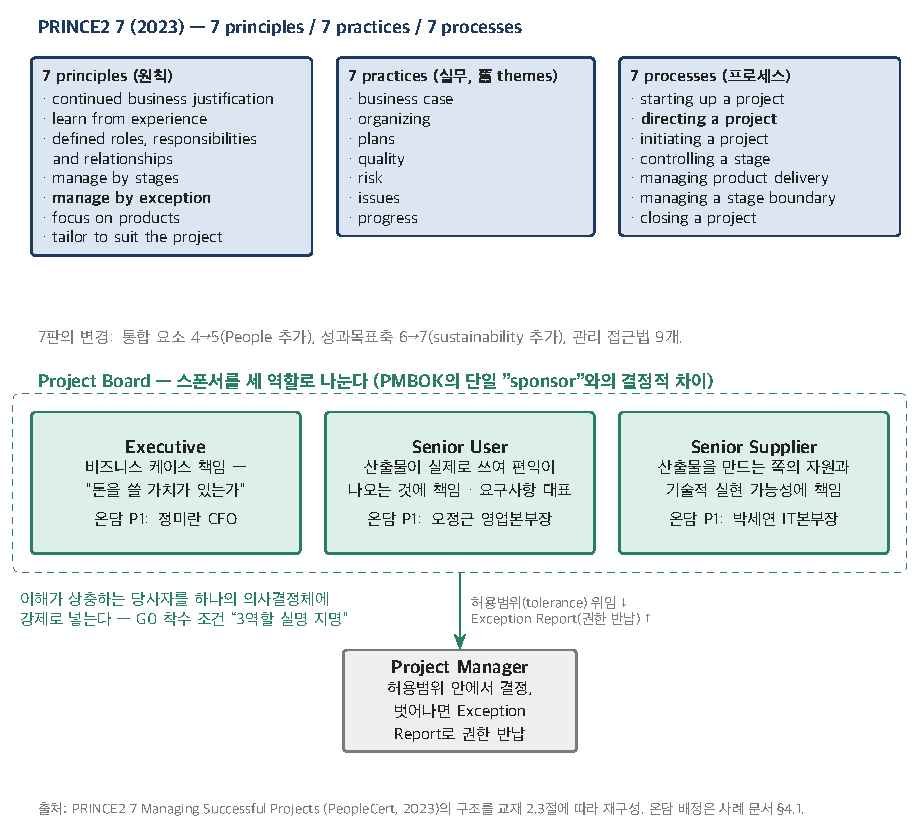
\includegraphics[width=1.00\textwidth,height=0.72\textheight,keepaspectratio]{../그림/PM_Day1/fig_2_3_prince2.pdf}
\par\nobreak\vspace{1pt}{\scriptsize\color{mDarkTeal!70}그림 2-4. PRINCE2 7 삼중 구조 + Project Board 3역할 (온담 배정)\par}
\end{center}
\framebreak
\par\smallskip\noindent{\usebeamercolor[fg]{normal text}\textbf{Project Board — 스폰서를 세 역할로 나눈다}\par}\nobreak
{\usebeamercolor[fg]{normal text}\small\setlength{\tabcolsep}{3pt}\renewcommand{\arraystretch}{1.12}
\begin{tabular}{@{}>{\raggedright\arraybackslash}p{0.194\textwidth}>{\raggedright\arraybackslash}p{0.627\textwidth}>{\raggedright\arraybackslash}p{0.164\textwidth}@{}}
\toprule
\textbf{역할} & \textbf{책임} & \textbf{온담 P1} \\
\midrule
\textbf{Executive} & 비즈니스 케이스 — "돈을 쓸 가치가 있는가" & 정미란 CFO \\
\textbf{Senior User} & 산출물이 \textbf{사용되어 편익이 나오는 것}. 요구사항 대표, 편익 실현 책무 & 오정근 영업본부장 \\
\textbf{Senior Supplier} & 산출물을 만드는 쪽의 자원·기술적 실현 가능성 & 박세연 IT본부장 \\
\bottomrule
\end{tabular}}
\par\smallskip
\begin{itemize}
\item\relax 이해가 상충하는 당사자를 \textbf{강제로 한 의사결정체에} 넣는다. 한국 프로젝트가 표류하는 이유는 스폰서가 없어서가 아니라 사용자 대표와 공급자 대표가 같은 테이블에 앉지 않아서
\end{itemize}
\par\smallskip\noindent{\usebeamercolor[fg]{normal text}\textbf{Manage by Exception — 허용범위 안에서는 보고하지 않을 권리}\par}\nobreak
\begin{itemize}
\item\relax 7 성과목표축(benefits, cost, time, quality, scope, sustainability, risk) $\times$ 3계층(project / stage / work package)의 \textbf{허용범위(tolerance) 격자}
\item\relax 벗어날 것으로 \textbf{예측되는 순간} Exception Report로 권한을 상위에 되돌린다 — "문제 보고서"가 아니라 \textbf{권한 반납 문서}
\item\relax 한국 조직에 주는 실익은 보고 규율 강화가 아니라 그 반대 — 주간·수시보고 문화의 비용을 줄이고 \textbf{PM의 자율성을 규정으로 방어하는 유일한 수단}
\end{itemize}
\note{§2.3 "PMBOK과의 결정적 차이" 앞 두 장치. 온담 G0 착수 조건에 "3역할 실명 지명"이 들어 있는 이유. 허용범위 초안(원가 +6\% = 10.08억 / 일정 +15영업일 / 범위 $\pm$35건 / EMV 8억 / 편익 $-$5\%p)은 5교시 §3.4에서 표로 다시 본다. "운영위 명단에 3역할을 배정해 보라 — 배정 안 되는 인물(대개 절반)과 비어 있는 역할(대개 Senior Supplier)이 거버넌스 결함"(생각해 볼 질문 2). 예상 소요 7분.}
\end{frame}

% ---- md slide 27: PRINCE2 장치 ③ Product-Based Planning · ④ 살아 있는 Business Case
\begin{frame}[allowframebreaks=1.0]{PRINCE2 장치 ③ Product-Based Planning · ④ 살아 있는 Business Case}
\small
\par\smallskip\noindent{\usebeamercolor[fg]{normal text}\textbf{Product-Based Planning — 활동이 아니라 산출물부터}\par}\nobreak
\begin{itemize}
\item\relax Project Product Description $\rightarrow$ Product Breakdown Structure $\rightarrow$ Product Descriptions $\rightarrow$ Product Flow Diagram
\item\relax 각 Product Description에 \textbf{품질 기준·검수 방법·검수 책임자}를 강제로 적게 한다
\item\relax 활동 중심 WBS("설계하기", "개발하기")는 검수 기준이 계획에서 누락되게 만든다 — 한국 SI·건설 검수 분쟁의 원인 대부분. \textbf{PBS 노드는 명사여야 하고, 명사가 아니면 검수할 수 없다} $\rightarrow$ Day2 WBS에서 실습
\end{itemize}
\par\smallskip\noindent{\usebeamercolor[fg]{normal text}\textbf{Business Case — 승인용 문서가 아니라 단계 경계마다 갱신}\par}\nobreak
\begin{itemize}
\item\relax 첫 원칙이 continued business justification. 각 stage 경계에서 "계속할 이유가 아직 있는가"를 Board가 되묻는다
\item\relax 편익 실현 책무는 Senior User, 정당성 유지는 Executive. 편익 검토는 종료 \textbf{이후}에 예약 — 온담 이사회 조건 3항과 G5(2028-03-31)
\end{itemize}
\par\smallskip\noindent{\usebeamercolor[fg]{normal text}\textbf{실무에서 어떻게 틀리는가} — 허용범위 없이 Exception Report 양식만 도입 / 허용범위를 전 프로젝트 공통 $\pm$10\%로 (편익 민감도에서 역산해야) / PBS를 동사로 채움 / PMBOK CCB(권한 회수)와 PRINCE2 Change Authority(권한 위임)를 섞음 — 온담 3층 변경 통제가 의도적으로 섞어 놓았고 Day3에서 그 비용을 확인\par}\nobreak
\note{§2.3 뒤 두 장치, "한국에서 PRINCE2가 실무에 주는 것", "실무에서 어떻게 틀리는가". 온담의 "본부장 위임전결 5억"과 "원가 허용범위 10.08억"이 서로 맞지 않는다는 불일치를 찾는 것이 격자의 첫 용도. 해외 발주처 대응에서 Highlight / End Stage / Exception Report, PID라는 이름을 아는 것의 값. 예상 소요 6분.}
\end{frame}

% ---- md slide 28: ISO 21502:2020 — 계약서가 인용하는 표준
\begin{frame}[allowframebreaks=1.0]{ISO 21502:2020 — 계약서가 인용하는 표준}
\small
\begin{itemize}
\item\relax 『Project, programme and portfolio management — Guidance on project management』, ISO/TC 258. \textbf{자격시험이 없다} $\rightarrow$ 교육시장에서 무명
\item\relax 그러나 글로벌 EPC·발주처 계약서와 RFP에서는 "PMBOK 준거"보다 자주 등장 — \textbf{중립성}. 발주처 PMI, 시공사 PRINCE2, 본사 자체 방법론일 때 유일하게 인용 가능한 표준
\item\relax 구조: §4 맥락 $\rightarrow$ §5 전제 조건(사업 정당성, 거버넌스) $\rightarrow$ §6 통합 실무(\textbf{§6.2 pre-project}, 착수, 통제, 종료, \textbf{§6.9 post-project}) $\rightarrow$ §7 관리 실무 17종
\par\nobreak
\begin{itemize}
\item\relax 프로젝트의 앞과 뒤를 표준 안에 넣었다 — Morris의 front-end 주장과 편익 관리를 표준 수준에서 수용
\end{itemize}
\item\relax \textbf{ISO 21500의 함정}: 2012년판 제목이 "Guidance on project management"였으나 2021년판은 "\textbf{Context and concepts}" $\rightarrow$ "ISO 21500에 따라 관리한다"는 지금 \textbf{무의미한 문장}. 지침은 21502, 용어는 \textbf{21506:2024}
\item\relax 계열: 21503(프로그램, 2022) / 21504(포트폴리오, 2022) / \textbf{21505:2017 거버넌스} / 21511:2018 WBS / 21508:2018 EVM(2판 2026 예정) / 21512:2024 EVM 구현
\end{itemize}
\note{§2.4 전체. 계약을 새로 쓸 때는 "ISO 21502:2020 §7 관리 실무에 따라"처럼 문서·연도·조항을 특정하라는 처방. 21505 거버넌스는 이사회·오너 계층 책무를 다루는 유일한 ISO 문서 — PRINCE2 Project Board를 "표준 근거 있는 것"으로 정당화할 때 인용하면 경영진 설득력이 달라진다. 21502는 계약과 감리의 언어이지 팀의 언어가 아니다. 예상 소요 7분.}
\end{frame}

% ---- md slide 29: 애자일·SAFe·하이브리드의 위치 — 표준의 반대편이 아니다
\begin{frame}[allowframebreaks=1.0]{애자일·SAFe·하이브리드의 위치 — 표준의 반대편이 아니다}
\small
\begin{center}\usebeamercolor[fg]{normal text}
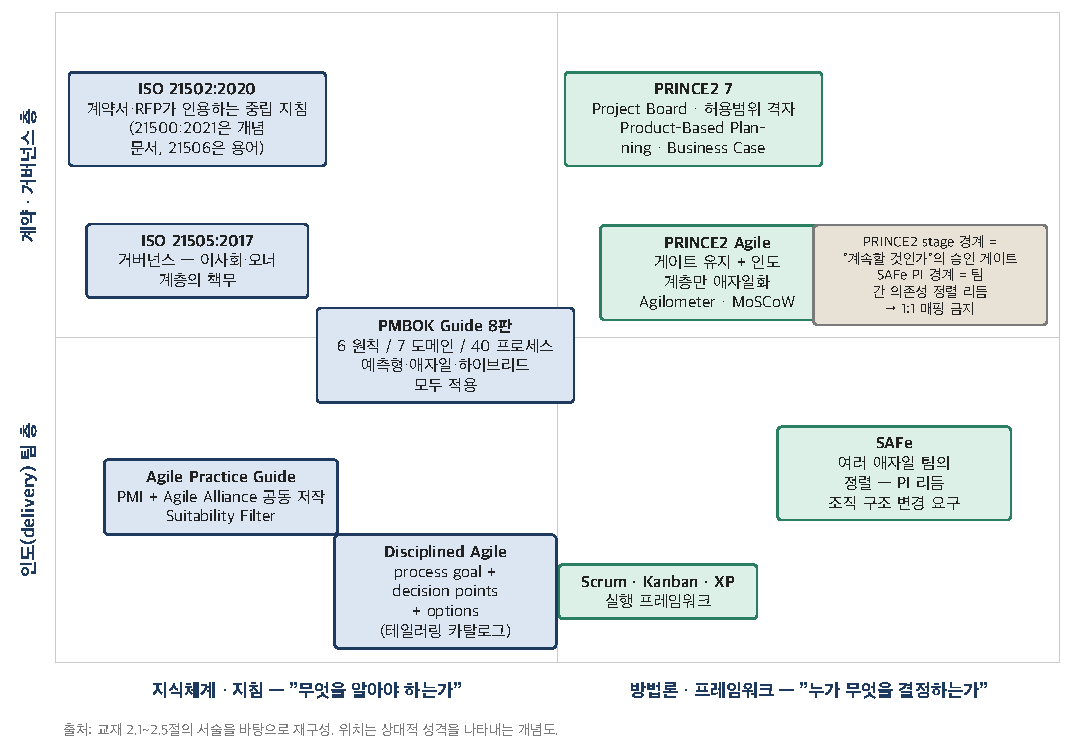
\includegraphics[width=1.00\textwidth,height=0.72\textheight,keepaspectratio]{../그림/PM_Day1/fig_2_4_standards_map.pdf}
\par\nobreak\vspace{1pt}{\scriptsize\color{mDarkTeal!70}그림 2-5. 표준 지형도 — 지식체계/방법론 $\times$ 거버넌스/인도 층\par}
\end{center}
\framebreak
\begin{itemize}
\item\relax 애자일(Scrum, Kanban, XP / SAFe, LeSS, Nexus, DA)은 PMBOK·PRINCE2·ISO와 같은 층위의 "표준"이 아니라, 그 표준들이 \textbf{개발 접근(development approach)}이라 부르는 것의 한 종류
\item\relax \textbf{Agile Practice Guide (2017)} — PMI 단독이 아니라 \textbf{Agile Alliance 공동 저작}. 실무 자산은 \textbf{Suitability Filter} (문화·팀·프로젝트 3범주 방사형 그림)
\item\relax \textbf{PRINCE2 Agile} — SAFe와 반대 방향. 게이트 거버넌스(Board, stage, 허용범위)를 유지하고 \textbf{인도 계층만 애자일화}. 시간·비용 고정, 범위를 MoSCoW로 유연하게. 한국 대기업이 게이트를 버릴 수 없을 때 유일한 표준급 절충
\item\relax \textbf{Disciplined Agile} — PMI가 2019 인수. process goal + decision points + options — 테일러링을 선택지 카탈로그로 조작화
\item\relax \textbf{SAFe} — 한국 실패 원인은 대부분 Boehm-Turner의 Personnel·Culture 축을 무시하고 프로세스만 이식. \textbf{PI $\neq$ Stage} — stage 경계는 "계속할 것인가"의 승인 게이트, PI 경계는 팀 간 정렬 리듬. 1:1로 매핑해 End Stage Report·갱신된 Business Case를 없애면 \textbf{중단 결정 지점이 조직에서 사라진다}
\item\relax \textbf{온담 P1의 하이브리드} — 스프린트 36회로 인도, 요구사항 월 1회 동결, FP 12,400점 고정가, 게이트 G0\textasciitilde{}G4 승인. 사업 정당성 재확인은 게이트(G1·G2·G3)에, 팀 간 정렬은 스프린트 경계와 월 동결에
\end{itemize}
\note{§2.5 전체. 오류 둘: "애자일이 waterfall을 대체했다"는 교체 서사 (Lenfle \& Loch 2010 — 맨해튼·폴라리스는 원래 병렬 실험이었고 표준화 과정에서 통제만 남았다. 애자일은 신문물이 아니라 잃어버린 뿌리) / 하이브리드를 "스프린트 돌리면서 간트도 그리는 것"으로 이해 — 하이브리드는 어느 결정을 언제 되돌릴 수 있게 남기고 언제 동결하는가의 \textbf{설계}. 예상 소요 8분.}
\end{frame}

% ---- md slide 30: 테일러링의 기준은 하나 — 되돌림 비용
\begin{frame}[allowframebreaks=1.0]{테일러링의 기준은 하나 — 되돌림 비용}
\small
\begin{center}\usebeamercolor[fg]{normal text}
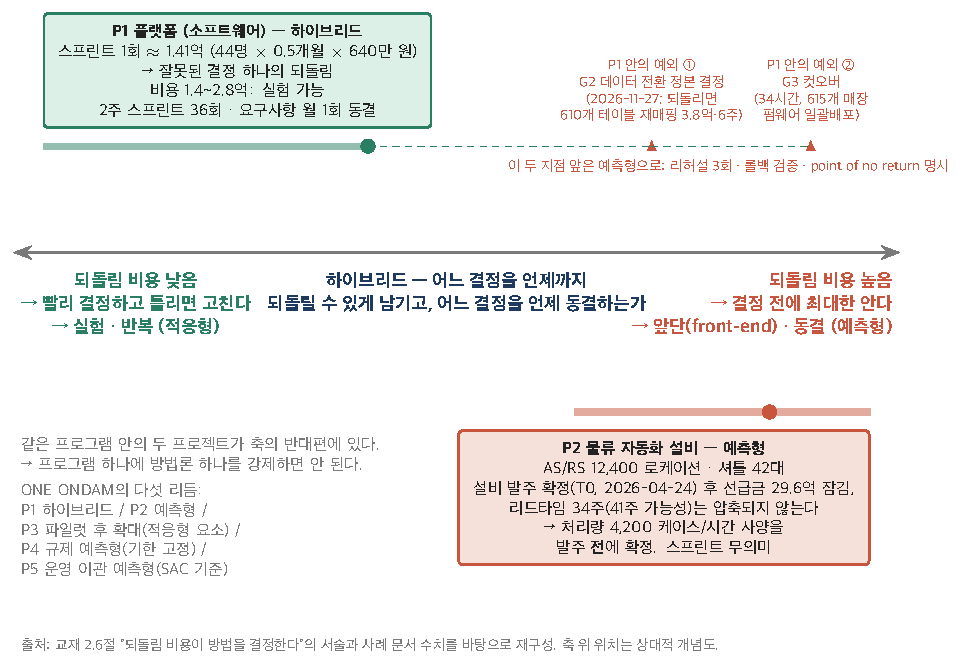
\includegraphics[width=1.00\textwidth,height=0.72\textheight,keepaspectratio]{../그림/PM_Day1/fig_2_6_reversal_axis.pdf}
\par\nobreak\vspace{1pt}{\scriptsize\color{mDarkTeal!70}그림 2-6. 되돌림 비용 축 위의 P1 vs P2\par}
\end{center}
\framebreak
\begin{itemize}
\item\relax 표준 셋(PMBOK 7·8, PRINCE2 7, ISO 21502) 모두 테일러링을 요구하지만 \textbf{판단 도구를 주지 않는다}
\item\relax 가장 단순하고 강력한 기준: \textbf{결정을 되돌리는 데 얼마가 드는가.} 적응형과 예측형은 이념이 아니라 되돌림 비용에 대한 두 개의 합리적 반응
\end{itemize}
{\usebeamercolor[fg]{normal text}\footnotesize\setlength{\tabcolsep}{3pt}\renewcommand{\arraystretch}{1.12}
\begin{tabular}{@{}>{\raggedright\arraybackslash}p{0.068\textwidth}>{\raggedright\arraybackslash}p{0.561\textwidth}>{\raggedright\arraybackslash}p{0.356\textwidth}@{}}
\toprule
 & \textbf{P1 — 소프트웨어} & \textbf{P2 — 물류 자동화 설비} \\
\midrule
되돌림 비용 & 스프린트 1회 $\approx$ 1.41억 (44명 $\times$ 0.5개월 $\times$ 640만 원). 잘못된 결정 하나 = 1\textasciitilde{}2 스프린트 = 1.4\textasciitilde{}2.8억 $\rightarrow$ \textbf{실험 가능} & 설비 발주(T0 2026-04-24) 후 선급금 \textbf{29.6억} 잠김, 리드타임 34주(41주 가능) 압축 불가 \\
처방 & 2주 스프린트, 월 단위 동결 & \textbf{예측형}. 앞단(설계 성숙도, 처리량 4,200 검증, 사양 동결)에 시간 \\
예외 & 되돌릴 수 없는 두 지점 — G2 데이터 전환 정본(재매핑 3.8억·6주), G3 컷오버(34시간) $\rightarrow$ 이 앞은 예측형: 리허설 3회, 롤백 검증, point of no return 명시 & 스프린트 무의미 — 설비 벤더는 2주마다 인도하지 않는다 \\
\bottomrule
\end{tabular}}
\par\smallskip
\begin{itemize}
\item\relax 결론: \textbf{프로그램 하나에 방법론 하나를 강제하면 안 된다.} P1 하이브리드 / P2 예측형 / P3 파일럿$\rightarrow$확대 / P4 예측형(기한 고정) / P5 예측형(SAC). 프로그램 운영위의 일은 이 다섯 리듬을 \textbf{통역}하는 것
\end{itemize}
\note{§2.6 "개념"과 "되돌림 비용이 방법을 결정한다". 1교시 §1.5 표의 "되돌림 비용" 열이 여기서 테일러링 규칙으로 승격된다. 생각해 볼 질문 3("여러분 프로젝트에서 되돌릴 수 없는 결정은 무엇이고 그 앞에 얼마나 시간을 쓰는가"). 예상 소요 7분.}
\end{frame}

% ---- md slide 31: Boehm-Turner 5축 (2003) — 축이 갈리면 시스템을 쪼개라
\begin{frame}[allowframebreaks=1.0]{Boehm-Turner 5축 (2003) — 축이 갈리면 시스템을 쪼개라}
\small
\begin{center}\usebeamercolor[fg]{normal text}
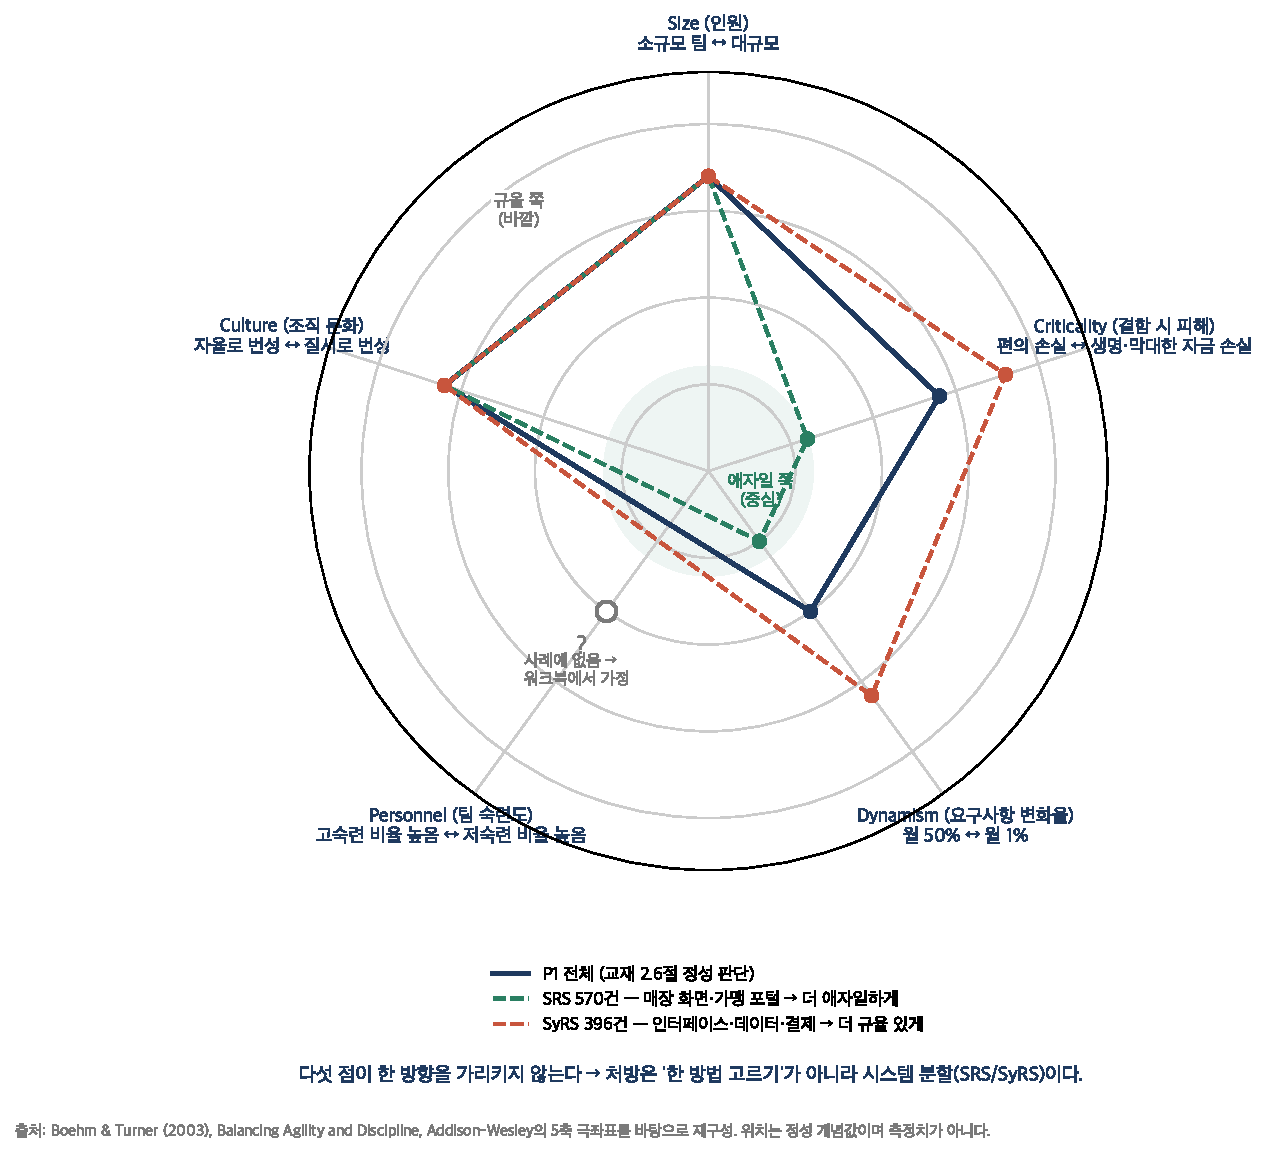
\includegraphics[width=1.00\textwidth,height=0.72\textheight,keepaspectratio]{../그림/PM_Day1/fig_2_6_boehm_turner.pdf}
\par\nobreak\vspace{1pt}{\scriptsize\color{mDarkTeal!70}그림 2-7. Boehm-Turner 5축 극좌표 — P1 전체와 SRS/SyRS 분할\par}
\end{center}
\framebreak
{\usebeamercolor[fg]{normal text}\small\setlength{\tabcolsep}{3pt}\renewcommand{\arraystretch}{1.12}
\begin{tabular}{@{}>{\raggedright\arraybackslash}p{0.165\textwidth}>{\raggedright\arraybackslash}p{0.167\textwidth}>{\raggedright\arraybackslash}p{0.207\textwidth}>{\raggedright\arraybackslash}p{0.447\textwidth}@{}}
\toprule
\textbf{축} & \textbf{애자일 쪽 (중심)} & \textbf{규율 쪽 (바깥)} & \textbf{P1 진단} \\
\midrule
\textbf{Size} & 소규모 & 대규모 & 피크 82명 $\rightarrow$ 바깥 \\
\textbf{Criticality} & 편의 손실 & 생명·막대한 자금 손실 & 615개 매장 결제 $\rightarrow$ 중간\textasciitilde{}바깥 \\
\textbf{Dynamism} & 월 50\% 변화 & 월 1\% 변화 & 월 동결 $\rightarrow$ 중간 \\
\textbf{Personnel} & 고숙련 비율 높음 & 저숙련 비율 높음 & 수행사 61명 분포 미상 $\rightarrow$ 워크북에서 가정 \\
\textbf{Culture} & 자율로 번성 & 질서로 번성 & 기관투자자 시계, 5,000만 원 CFO 결재 $\rightarrow$ 질서 쪽 \\
\bottomrule
\end{tabular}}
\par\smallskip
\begin{itemize}
\item\relax 진짜 처방은 "한 방법을 골라라"가 아니라 \textbf{축이 서로 다른 방향을 가리키면 시스템을 쪼개서 부분마다 다른 방법을 써라}
\item\relax P1에 적용: 매장 화면·가맹 포털(SRS 570건, dynamism 높음·criticality 낮음)은 \textbf{더 애자일하게} / 인터페이스·데이터·결제(SyRS 396건, criticality 높음·dynamism 낮음)는 \textbf{더 규율 있게} — 영업본부 vs IT본부 우선순위 긴장을 방법론 수준에서 해소하는 한 답
\item\relax 한국에서 결정적인 축은 \textbf{Personnel과 Culture} — 애자일 전환은 거의 항상 이 둘을 무시하고 프로세스만 이식해서 실패
\end{itemize}
\note{§2.6 "Boehm-Turner 5축". 2003년 문헌인데 2026년 SAFe 실패 분석에 가장 잘 맞는다. 5축 결과를 "애자일 점수"로 환산해 조직 전체에 하나를 강제하는 것은 원저의 결론과 정반대. 워크북 §3 심화 과제(SRS/SyRS 분할 근거)가 이 슬라이드다. 생각해 볼 질문 4. 예상 소요 6분.}
\end{frame}

% ---- md slide 32: Cynefin — 방법론 선택 도구가 아니다 (Snowden & Boone, 2007 HBR)
\begin{frame}[allowframebreaks=1.0]{Cynefin — 방법론 선택 도구가 아니다 (Snowden \& Boone, 2007 HBR)}
\small
\begin{center}\usebeamercolor[fg]{normal text}
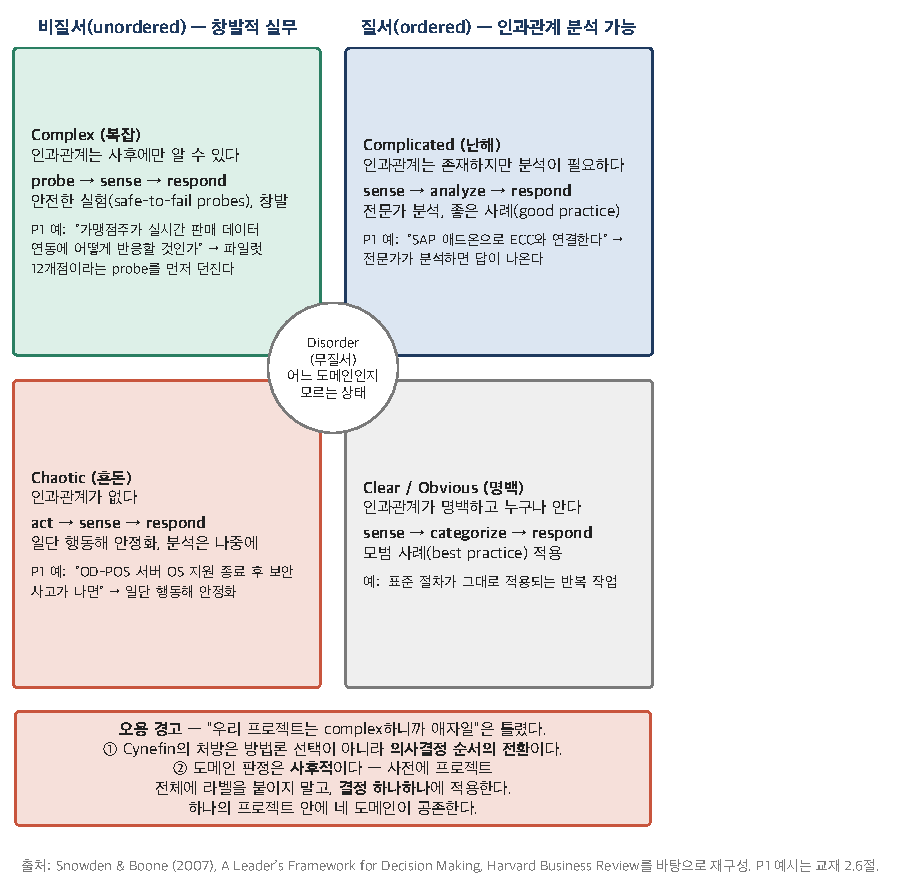
\includegraphics[width=1.00\textwidth,height=0.72\textheight,keepaspectratio]{../그림/PM_Day1/fig_2_6_cynefin.pdf}
\par\nobreak\vspace{1pt}{\scriptsize\color{mDarkTeal!70}그림 2-8. Cynefin 네 도메인과 의사결정 순서 — P1 결정 예시\par}
\end{center}
\framebreak
{\usebeamercolor[fg]{normal text}\small\setlength{\tabcolsep}{3pt}\renewcommand{\arraystretch}{1.12}
\begin{tabular}{@{}>{\raggedright\arraybackslash}p{0.164\textwidth}>{\raggedright\arraybackslash}p{0.167\textwidth}>{\raggedright\arraybackslash}p{0.305\textwidth}>{\raggedright\arraybackslash}p{0.349\textwidth}@{}}
\toprule
\textbf{도메인} & \textbf{인과관계} & \textbf{의사결정 순서} & \textbf{실무} \\
\midrule
Clear (obvious) & 명백 & sense $\rightarrow$ categorize $\rightarrow$ respond & best practice \\
Complicated & 있지만 분석 필요 & sense $\rightarrow$ analyze $\rightarrow$ respond & 전문가 분석, good practice \\
Complex & 사후에만 알 수 있음 & \textbf{probe $\rightarrow$ sense $\rightarrow$ respond} & 안전한 실험(safe-to-fail probes), 창발 \\
Chaotic & 없음 & act $\rightarrow$ sense $\rightarrow$ respond & 일단 행동해 안정화 \\
\bottomrule
\end{tabular}}
\par\smallskip
\begin{itemize}
\item\relax 가장 흔한 오용: "우리 프로젝트는 complex하니까 애자일" — 두 가지로 틀렸다
\par\nobreak
\begin{enumerate}
\item\relax Cynefin의 처방은 방법론 선택이 아니라 \textbf{의사결정 양식의 전환}
\item\relax \textbf{도메인 판정은 사후적} — 사전에 "이 프로젝트는 complex"라고 라벨 붙이는 것은 프레임워크의 논지에 어긋난다
\end{enumerate}
\item\relax 올바른 용법: 프로젝트 전체가 아니라 \textbf{결정 하나하나}에 — "SAP 애드온으로 ECC 연결" = complicated / "가맹점주가 실시간 판매 데이터 연동에 어떻게 반응할까" = complex $\rightarrow$ 파일럿 12개점이라는 probe / "OD-POS OS 종료 후 보안 사고" = chaotic
\item\relax Stacey matrix: 세간의 2$\times$2는 \textbf{Ralph Stacey 본인이 후속 저작에서 폐기}했다. 쓸 거라면 그 사실을 먼저 말해야 한다
\end{itemize}
\note{§2.6 "Cynefin". 하나의 프로젝트 안에 네 도메인이 공존하며 PM의 일은 지금 다루는 결정이 어느 도메인인지 감각하고 순서를 바꾸는 것. 경력 있는 청중 앞에서 Stacey 한마디가 신뢰를 만든다. 예상 소요 5분.}
\end{frame}

% ---- md slide 33: 테일러링을 문서로 남기기 — TDR 네 칸
\begin{frame}[allowframebreaks=1.0]{테일러링을 문서로 남기기 — TDR 네 칸}
\small
\begin{itemize}
\item\relax 세 도구는 \textbf{다른 질문}에 답한다: NTCP = 프로젝트 유형 / Boehm-Turner = 팀·조직의 준비도 / Cynefin = 개별 결정의 성격. 서로 다른 답을 줄 때 하나를 고르지 말라 — \textbf{충돌 지점이 설계할 지점}
\item\relax 근거 기록이 없으면 사내 감사·외부 감리에서 모든 생략이 "표준 미준수"로 잡히고, PMO는 방어를 위해 문서를 다 만들게 된다 — \textbf{한국 조직에서 문서가 줄지 않는 진짜 메커니즘}
\item\relax \textbf{테일러링 결정 기록 (Tailoring Decision Record, TDR)} — 생략·조정한 프로세스·산출물마다 한 행
\end{itemize}
{\usebeamercolor[fg]{normal text}\small\setlength{\tabcolsep}{3pt}\renewcommand{\arraystretch}{1.12}
\begin{tabular}{@{}>{\raggedright\arraybackslash}p{0.302\textwidth}>{\raggedright\arraybackslash}p{0.328\textwidth}>{\raggedright\arraybackslash}p{0.238\textwidth}>{\raggedright\arraybackslash}p{0.116\textwidth}@{}}
\toprule
\textbf{무엇을} & \textbf{왜} & \textbf{어떤 리스크를 수용하는가} & \textbf{누가 승인했는가} \\
\midrule
(예) 스프린트 단위 상세 일정표 생략 & 월 동결·게이트로 통제 & 스프린트 내 지연 가시성 저하 & 스폰서 \\
(예) 데이터 전환 리허설 3회 \textbf{추가} & 2023 감사 지적 "형상관리 미비", G2 비가역성 & 시험 기간 압박 & 스폰서 \\
\bottomrule
\end{tabular}}
\par\smallskip
\begin{itemize}
\item\relax 서술 문단으로 처리하면 안 된다 — 생략 항목별로 행이 있어야 감사 조항에 대응된다
\item\relax 테일러링은 줄이는 것만이 아니다 — P1의 리허설 3회, 외부 감리 4.2억, 발주사 PMO 3명은 표준이 아니라 \textbf{온담의 과거 실패가 요구하는 추가}
\end{itemize}
\note{§2.6 "테일러링을 문서로 남기기"와 "실무에서 어떻게 틀리는가". 워크북 §3에서 P1의 TDR을 작성한다고 되어 있으나 이 워크북 판본의 §3은 이해관계자 등록부이므로, TDR은 Day2 워크북 또는 심화 과제로 안내한다. 예상 소요 5분.}
\end{frame}

% ---- md slide 34: 자격 체계의 실효성 — 문을 여는 열쇠이지 판단을 대신하지 않는다
\begin{frame}[allowframebreaks=1.0]{자격 체계의 실효성 — 문을 여는 열쇠이지 판단을 대신하지 않는다}
\small
{\usebeamercolor[fg]{normal text}\footnotesize\setlength{\tabcolsep}{3pt}\renewcommand{\arraystretch}{1.12}
\begin{tabular}{@{}>{\raggedright\arraybackslash}p{0.091\textwidth}>{\raggedright\arraybackslash}p{0.123\textwidth}>{\raggedright\arraybackslash}p{0.243\textwidth}>{\raggedright\arraybackslash}p{0.528\textwidth}@{}}
\toprule
\textbf{자격} & \textbf{발급} & \textbf{기반 문서} & \textbf{실효} \\
\midrule
\textbf{PMP} & PMI & \textbf{ECO} (PMBOK은 참고 문헌 중 하나). 2026-07-09 신버전 & 한국 최고 인지도, 공공 정보화 가점, 대기업 PMO 채용 요건. 증명하는 것은 "지식과 경력 시간"이지 "상황 속 판단"이 아님 \\
PMI-ACP & PMI & 애자일 실무 &  \\
PRINCE2 7 F/P & PeopleCert & PRINCE2 7 매뉴얼 & 한국 자격 가치 낮음. 영국·EU·중동 발주처·글로벌 본사 보고에서 "문서 이름 맞추는 능력" \\
SAFe SA/SSM/SPC & Scaled Agile & SAFe & 전환 컨설팅 수임에 유리, 개인 급여 프리미엄은 PMP보다 낮은 경향, 연 1회 갱신 \\
IPMA A\textasciitilde{}D & IPMA & \textbf{ICB4} 29 역량 요소 & 자격 실효는 낮으나 ICB4 문서는 사내 PM 등급제·직무기술서의 원천으로 가치 \\
\bottomrule
\end{tabular}}
\par\smallskip
\begin{itemize}
\item\relax "PMP를 8판으로 다시 봐야 하나요?" $\rightarrow$ \textbf{아니오, 질문 자체가 틀렸다.} 시험 근거는 ECO. 판본 논쟁은 자격이 아니라 \textbf{사내 문서 체계} 문제
\item\relax 사내 교육을 PMBOK 목차에 맞추면 합격률은 오히려 역효과. 자격을 "역량 증명"으로 승진에 쓰면 자격은 있으나 판단이 없는 PM을 승진시킨다
\end{itemize}
\note{§2.7 전체. Crawford, Morris, Thomas, Winter(2006) — 자격 기반 역량 모델은 trained technician을 측정하며 성과는 reflective practitioner의 판단에서 나온다(마무리 §4.1 방향 5). 반대로 자격 무용론도 오류 — 원 논문의 주장은 대체가 아니라 발달 경로이고, 자격은 공통 어휘를 얻는 가장 빠른 길. Business Environment 배점 상승은 2차 출처이므로 숫자 단정 금지. 예상 소요 5분.}
\end{frame}

% ---- md slide 35: 2교시 핵심 정리
\begin{frame}[allowframebreaks=1.0]{2교시 핵심 정리}
\small
\begin{enumerate}
\item\relax PMBOK은 6판(49 프로세스/ITTO) $\rightarrow$ 7판(12원칙/8도메인, 프로세스 삭제) $\rightarrow$ 8판(6원칙/7도메인/5 Focus Areas/40 프로세스, \textbf{부분 회귀}). 회귀는 프로세스 없는 표준을 조직이 쓸 수 없다는 피드백의 결과
\item\relax 한국 사내 표준은 대부분 6판. 처방은 재작성이 아니라 \textbf{4열 재매핑 대장}. Integration$\rightarrow$Governance, Cost$\rightarrow$Finance, Quality·Communications·Procurement 소멸이 실질 변경
\item\relax PRINCE2의 자산은 \textbf{3역할} / \textbf{허용범위 격자와 Manage by Exception} / \textbf{Product-Based Planning} / \textbf{단계마다 갱신되는 Business Case}
\item\relax 계약서는 ISO 21502를 인용한다. "ISO 21500에 따라"는 2021년 이후 틀린 문장 — 지침 21502, 용어 21506
\item\relax 애자일은 개발 접근의 한 종류. PRINCE2 Agile은 게이트를 유지하고 인도만 애자일화. Stage $\neq$ PI
\item\relax 테일러링의 기준은 \textbf{되돌림 비용}. NTCP(유형) / Boehm-Turner(준비도, 갈리면 분할) / Cynefin(개별 결정)은 다른 질문. 결과는 \textbf{TDR 네 칸}으로
\item\relax PMP의 근거는 ECO. 자격은 문을 여는 열쇠
\end{enumerate}
\note{제2장 핵심 정리 그대로. 점심 전 마지막 슬라이드. 오후 4교시 실습을 위해 워크북 §0.3(온담 한 페이지 요약)과 §1.5·§2.5 완성 예시본을 점심시간에 훑어 오도록 안내한다. 예상 소요 3분.}
\end{frame}

\section{3교시 (90분) — 착수 이론: 비즈니스 케이스 · 편익의 소유 · 헌장 · 이해관계자}

% ---- md slide 36: 이 교시에서 배우는 것
\begin{frame}[allowframebreaks=1.0]{이 교시에서 배우는 것}
\small
\begin{itemize}
\item\relax 착수 이전 — 비즈니스 케이스와 편익의 소유권 [§3.1]
\par\nobreak
\begin{itemize}
\item\relax 착수 전에 이미 결정된 것들 / 비즈니스 케이스의 항목 / Zwikael \& Smyrk의 ITO / Ward \& Daniel의 BDN
\end{itemize}
\item\relax 프로젝트 헌장 — 항목별 의미와 한국 기업에서의 실질화 [§3.2]
\item\relax 이해관계자 — 식별·분석·참여 계획 [§3.3]
\par\nobreak
\begin{itemize}
\item\relax Power/Interest 격자의 한계 / Mitchell-Agle-Wood 현저성 모델 / 한국 특유의 이해관계자
\end{itemize}
\item\relax 4교시 실습 ①(비즈니스 케이스 요약 + 헌장)의 이론 부분
\end{itemize}
\note{제3장 §3.1\textasciitilde{}3.3. 시간 배분: §3.1 30분, §3.2 30분, §3.3 25분, 정리 5분. 오전보다 온담 숫자가 훨씬 많이 나온다 — 워크북 §0.3 한 페이지 요약을 펼쳐 놓고 듣게 한다. 예상 소요 2분.}
\end{frame}

% ---- md slide 37: 착수의 첫 번째 일은 검증이다 — 비즈니스 케이스를 온담 P1로 채우면
\begin{frame}[allowframebreaks=1.0]{착수의 첫 번째 일은 검증이다 — 비즈니스 케이스를 온담 P1로 채우면}
\small
\begin{itemize}
\item\relax 표준이 "착수 전"을 수용하는 방식: ISO 21502 \textbf{§6.2 pre-project activities} / PRINCE2 \textbf{Starting Up a Project}가 Initiating 앞에 / PMBOK 8판 Initiating은 프로세스 둘뿐(헌장 개발, 이해관계자 식별) — 입력인 BC·편익 관리 계획은 \textbf{프로젝트 바깥}에서 온다
\item\relax 착수의 첫 번째 일은 새로 만드는 것이 아니라 \textbf{이미 만들어진 BC의 숫자와 가정을 검증하는 것}. P1 PM이 받는 것: 이사회 부의안(2025-12) + 편익 표(연 214억) + 프로그램 관리 규정 + 승인 조건 5개항. 읽지 않고 헌장을 쓰는 것은 \textbf{남이 정한 목표를 자기가 정한 것처럼 서명하는 일}
\end{itemize}
\framebreak
{\usebeamercolor[fg]{normal text}\footnotesize\setlength{\tabcolsep}{3pt}\renewcommand{\arraystretch}{1.12}
\begin{tabular}{@{}>{\raggedright\arraybackslash}p{0.068\textwidth}>{\raggedright\arraybackslash}p{0.235\textwidth}>{\raggedright\arraybackslash}p{0.682\textwidth}@{}}
\toprule
\textbf{항목} & \textbf{무엇을 적는가} & \textbf{온담 P1에서} \\
\midrule
\textbf{문제 / 기회} & 무엇이 잘못되어 있고 얼마의 비용을 만드는가. 숫자로 & OD-POS 서버 OS 지원 종료(2024-07), 인터페이스 47본 중 문서 부재 13본, 재고 실시간 가시성 부재. 폐기율 3.9\% = 연 \textbf{98.7억}(2,530억 $\times$ 3.9\%), 결품률 4.7\%, 가맹 발주 리드타임 38시간 \\
\textbf{대안} & do-nothing / do-minimum / 제안안 / 그 밖. 각각의 비용·효과 & (a) 현행 유지 — 패치 없는 결제 시스템 + SAP ECC 2027-12 종료 시 이중 위기 (b) 부분 개선 (c) 통합 플랫폼(P1) (d) 상용 패키지 — 검토 기록 없음 \\
\textbf{편익} & 기준값·목표값·측정 방법·시점·\textbf{측정 책임자} & B-01\textasciitilde{}B-08, M+24 연 214억. 측정 책임자 "프로그램 착수 후 지정 예정" — \textbf{결함 ①} \\
\textbf{비용} & 프로젝트 + 운영 = TCO & P1 168억 + 나머지 260억. 연 운영비 27억(3년 81억)이 편익에서 \textbf{미차감} — \textbf{결함 ②} \\
\textbf{리스크} & 편익이 안 나올 주요 이유 & 과거 2건 중단·축소, P2 리드타임, 3PL WMS 개방, 가맹 부속서 388점 서면 동의, 규제 기한 \\
\textbf{권고} & 어느 대안을 왜. 승인 조건 & 이사회 원칙 승인 + 5개 조건 \\
\bottomrule
\end{tabular}}
\par\smallskip
\note{§3.1 "착수 전에 이미 결정된 것들"과 "비즈니스 케이스에는 무엇이 들어가는가". 1교시 Engwall이 표준에서 어떻게 자리 잡았는지로 연결. 표를 채우면서 알게 되는 것 — 온담 BC는 존재하지만 \textbf{완결되어 있지 않다}. 다음 슬라이드에서 결함을 목록화. 예상 소요 9분.}
\end{frame}

% ---- md slide 38: 온담 비즈니스 케이스의 결함 — PM이 고칠 것이 아니라 목록으로 만들 것
\begin{frame}[allowframebreaks=1.0]{온담 비즈니스 케이스의 결함 — PM이 고칠 것이 아니라 목록으로 만들 것}
\small
\begin{itemize}
\item\relax B-03 결품률: "기회손실, 미산정"
\item\relax B-02 재고 정확도 91.3\%: 분모가 \textbf{순환실사 대상 SKU 69\%}뿐
\item\relax B-06 물류 처리량 절감 96억: 이사회 자료에 \textbf{분모가 없고}, 노조가 "인원 절반이라는 뜻이냐"고 묻고 있으며, 한동석 본부장은 "4,200은 현장 숫자가 아니다"
\item\relax 편익 합계 214억에서 연 운영비 27억 미차감 $\rightarrow$ 정직한 숫자는 \textbf{187억}
\item\relax 측정 책임자: "추후 지정" — 그것은 지정하지 않겠다는 뜻
\item\relax CFO: "근거가 없는 항목은 승인하지 않겠다" / 내부감사: "편익 산정 근거를 문서로 제출하라"
\item\relax PM의 착수 시점 일은 결함을 고치는 것이 아니라(권한 밖) \textbf{결함을 목록으로 만들어 스폰서에게 결정을 요구하는 것}
\end{itemize}
\note{§3.1의 결함 문단과 "실무에서 어떻게 틀리는가". 오류 넷: BC를 승인용으로 한 번 쓰고 서랍에(좀비 프로젝트) / 편익을 종료와 함께 폐기(측정 불가) / Gate 1에서 5년 매출·전체 NPV 요구(허구 $\rightarrow$ survival of the unfittest; 게이트는 "다음 단계로 갈 권리를 사는 것") / 운영비 미차감. 4교시 워크북 §1 심화 과제가 이 결함 목록 + 결정 요청 문안. 예상 소요 6분.}
\end{frame}

% ---- md slide 39: 편익은 누가 소유하는가 — Zwikael & Smyrk의 ITO 모델 (2011)
\begin{frame}[allowframebreaks=1.0]{편익은 누가 소유하는가 — Zwikael \& Smyrk의 ITO 모델 (2011)}
\small
\begin{center}\usebeamercolor[fg]{normal text}
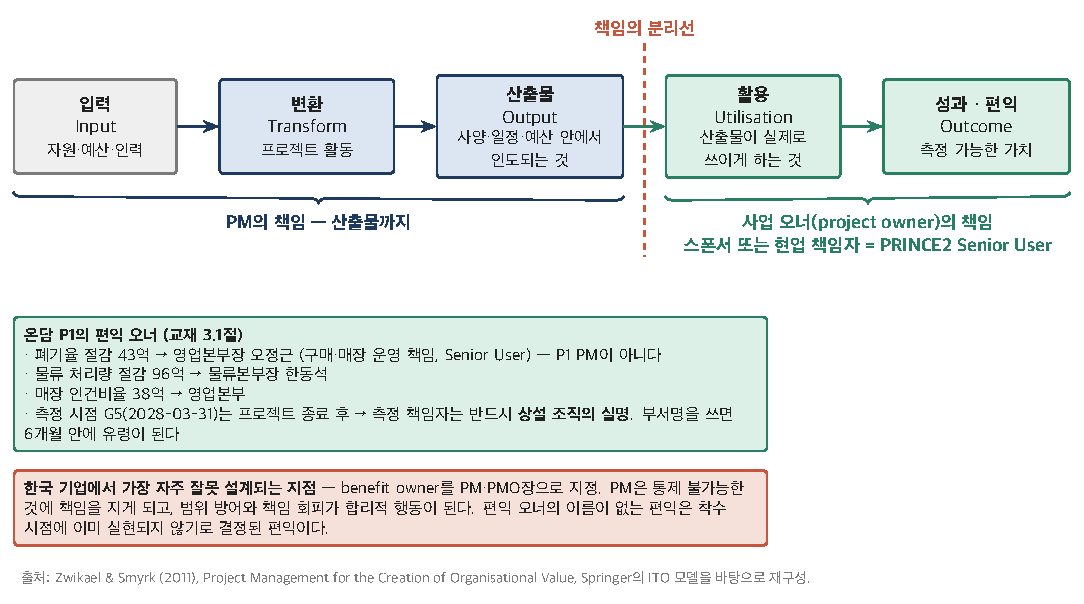
\includegraphics[width=1.00\textwidth,height=0.50\textheight,keepaspectratio]{../그림/PM_Day1/fig_3_1_ito.pdf}
\par\nobreak\vspace{1pt}{\scriptsize\color{mDarkTeal!70}그림 3-1. Zwikael \& Smyrk ITO 모델 — 책임의 분리선\par}
\end{center}
\begin{itemize}
\item\relax \textbf{산출물(output)} = PM의 책임 — 정해진 사양·일정·예산 안에서 인도
\item\relax \textbf{활용(utilisation)·성과(outcome)} = 사업 오너(스폰서 또는 현업 책임자)의 책임 — 실제로 쓰이게 하고 편익이 나오게
\item\relax PM에게 매출·절감 목표를 부여하면 $\rightarrow$ 통제 불가능한 것에 책임 $\rightarrow$ \textbf{범위 방어와 책임 회피가 합리적 행동}이 된다
\item\relax 한국 기업에서 가장 자주 잘못 설계되는 지점: benefit owner를 PM이나 PMO장으로 지정하는 것. PRINCE2가 편익 책무를 Senior User에게 두는 것도 같은 논리
\item\relax 온담: 폐기율 43억의 오너는 P1 PM이 아니라 \textbf{오정근 영업본부장}(Senior User) / 물류 처리량 96억은 \textbf{한동석} / 매장 인건비율 38억은 영업본부
\item\relax 편익 측정 시점(G5 2028-03-31)에 프로젝트 조직은 없다 $\rightarrow$ 측정 책임자는 반드시 \textbf{상설 조직의 실명}. 부서명을 쓰면 그 편익은 6개월 안에 유령이 된다
\end{itemize}
\note{§3.1 "편익은 누가 소유하는가". 1교시 임시조직론의 "제도화된 종료"가 왜 실명이어야 하는지의 근거. "편익 오너의 이름이 없는 편익은 착수 시점에 이미 실현되지 않기로 결정된 편익이다." 예상 소요 6분.}
\end{frame}

% ---- md slide 40: 편익 실현은 왜 대부분 실패하는가 — Ward & Daniel의 BDN
\begin{frame}[allowframebreaks=1.0]{편익 실현은 왜 대부분 실패하는가 — Ward \& Daniel의 BDN}
\small
\begin{itemize}
\item\relax 편익은 기술이 아니라 \textbf{조직 변화}에서 나오는데, 대부분의 프로젝트는 기술을 인도하고 끝난다
\item\relax \textbf{Benefits Dependency Network} — 투자 목적 $\leftarrow$ 편익 $\leftarrow$ 사업 변화 $\leftarrow$ 조력 변화 $\leftarrow$ IT 조력자를 \textbf{역방향}으로 연결
\end{itemize}
\begin{center}\usebeamercolor[fg]{normal text}
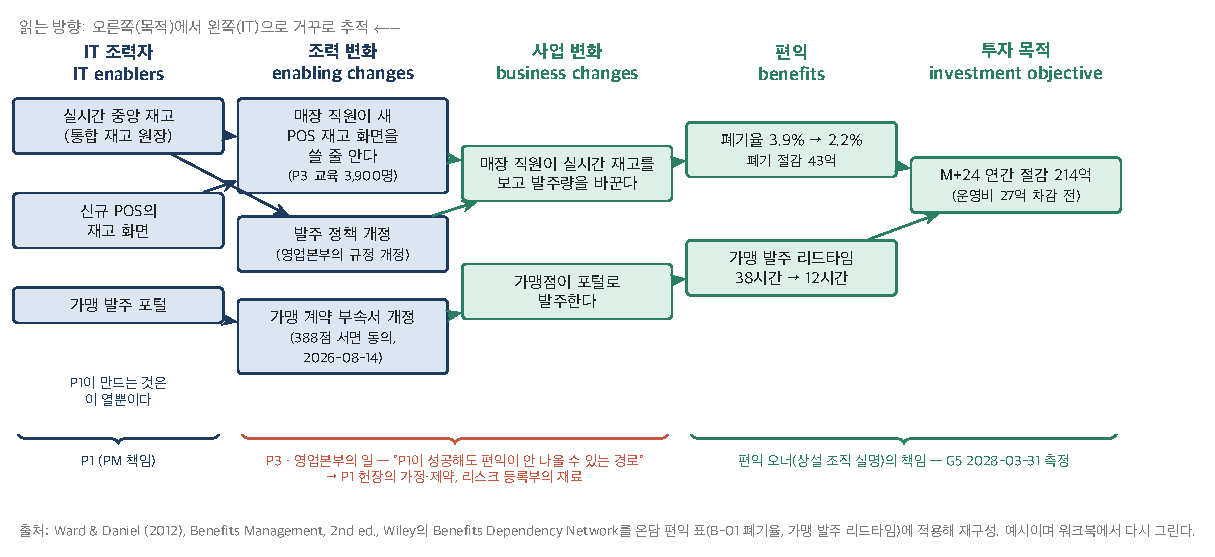
\includegraphics[width=1.00\textwidth,height=0.45\textheight,keepaspectratio]{../그림/PM_Day1/fig_3_1_bdn.pdf}
\par\nobreak\vspace{1pt}{\scriptsize\color{mDarkTeal!70}그림 3-2. 온담 편익의 BDN — 폐기율·가맹 발주 리드타임\par}
\end{center}
\begin{itemize}
\item\relax P1이 만드는 것은 \textbf{맨 왼쪽뿐}. 나머지는 P3와 영업본부의 일
\item\relax BDN은 "P1이 성공해도 편익이 안 나올 수 있는 경로"를 착수 시점에 보여 준다 $\rightarrow$ 헌장의 \textbf{가정·제약} 항목과 리스크 등록부의 재료
\item\relax Bradley 『Benefit Realisation Management』(2판, 2010) — benefit profile(편익마다 기준값·목표값·측정 방법·오너·시점 한 장), benefit owner 지정 절차
\end{itemize}
\note{§3.1 "편익 실현은 왜 대부분 실패하는가". 워크북 §1 편익 표의 "분모·기여 구분·측정 책임자" 열이 BDN과 benefit profile에서 왔다고 연결. 예상 소요 5분.}
\end{frame}

% ---- md slide 41: 프로젝트 헌장은 권한 문서다 — 항목별 의미 ① 목적 · 성공 기준 · 범위/제외
\begin{frame}[allowframebreaks=1.0]{프로젝트 헌장은 권한 문서다 — 항목별 의미 ① 목적 · 성공 기준 · 범위/제외}
\small
\begin{center}\usebeamercolor[fg]{normal text}
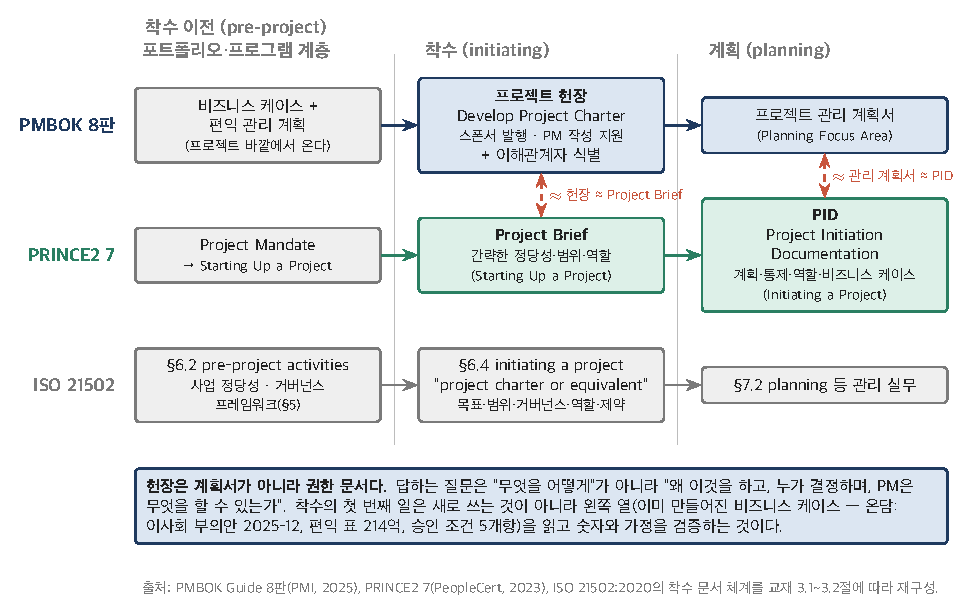
\includegraphics[width=1.00\textwidth,height=0.72\textheight,keepaspectratio]{../그림/PM_Day1/fig_3_2_doc_flow.pdf}
\par\nobreak\vspace{1pt}{\scriptsize\color{mDarkTeal!70}그림 3-3. 착수 문서 흐름 — 비즈니스 케이스 $\rightarrow$ 헌장 $\rightarrow$ 계획서, PRINCE2·ISO 대응\par}
\end{center}
\framebreak
\begin{itemize}
\item\relax 헌장 = 프로젝트의 존재를 공식화하고 \textbf{PM에게 조직 자원을 쓸 권한을 부여}하는 문서. 답하는 질문은 "무엇을 어떻게"가 아니라 \textbf{"왜 하고, 누가 결정하며, PM은 무엇을 할 수 있는가"}
\item\relax 표준 위치: PMBOK 8판 Initiating 첫 프로세스 Develop Project Charter의 출력(스폰서 발행, PM 작성 지원) / PRINCE2 7 \textbf{Project Brief}(Starting Up) $\rightarrow$ \textbf{PID}(Initiating) — PMBOK 헌장 $\approx$ Project Brief / ISO 21502 §6.4 "project charter or equivalent"
\end{itemize}
\par\smallskip\noindent{\usebeamercolor[fg]{normal text}\textbf{목적 / 정당성} — 사업 배경·해결할 문제·기대 효과를 3\textasciitilde{}5문장, \textbf{반드시 숫자}\par}\nobreak
\begin{itemize}
\item\relax 흔한 오류: \textbf{솔루션을 목적으로 적는 것.} "차세대 플랫폼을 구축한다"는 목적이 아니다
\item\relax 온담: "보안 패치가 중단된 시스템으로 615개 매장의 결제를 처리하고 있고, 재고를 실시간으로 볼 수 없어 연 약 98.7억어치 식자재가 폐기되며, 2027 IPO 예비심사 전에 이 상태를 벗어나야 한다" — \textbf{프로젝트가 없어져도 남는 문장}
\end{itemize}
\par\smallskip\noindent{\usebeamercolor[fg]{normal text}\textbf{측정 가능한 목표 / 성공 기준} — 두 층으로 분리\par}\nobreak
\begin{itemize}
\item\relax 프로젝트 관리 성공(PM 책임): "2027-05-29까지 156억 한도 내 다섯 산출물 인도, SAC 충족"
\item\relax 프로젝트 성공(편익 오너 책임): "M+24 폐기율 2.2\%, 결품률 1.5\%, 리드타임 12h — 측정 책임자 실명"
\item\relax 흔한 오류: 편익 목표를 PM의 성공 기준에 넣는 것
\end{itemize}
\par\smallskip\noindent{\usebeamercolor[fg]{normal text}\textbf{범위 / 제외 범위} — 무엇을 만드는가보다 \textbf{무엇을 만들지 않는가}가 더 중요. 제외 범위 없는 헌장은 범위 팽창의 초대장\par}\nobreak
\begin{itemize}
\item\relax P1 제외: SAP ECC 교체, 이천 설비·WMS(P2), 교육·가맹 계약 개정(P3), 규제 등록 자체(P4), 운영 조직(P5)
\item\relax 흔한 오류: "기타 협의된 사항"처럼 모호하게
\end{itemize}
\note{§3.2 "왜 쓰는가"와 "항목별 의미" 앞부분. 워크북 헌장은 Project Brief에 PID의 핵심(권한·허용범위·완료 기준)을 얹은 15개 항목. 상위 요구사항(5\textasciitilde{}10줄, 상세가 아님), 산출물(명사로 — PBP의 출발), 마일스톤(되돌릴 수 없는 지점 G2·G3와 외부 고정 기한을 구분)은 구두로 짧게. 워크북 §2.3에 15개 항목 전부의 "무엇을/어떻게/흔한 오류/온담에서는" 가이드가 있다고 안내. 예상 소요 10분.}
\end{frame}

% ---- md slide 42: 헌장 항목별 의미 ② — 예산 층 · 가정과 제약 · 거버넌스와 PM 권한
\begin{frame}[allowframebreaks=1.0]{헌장 항목별 의미 ② — 예산 층 · 가정과 제약 · 거버넌스와 PM 권한}
\small
\par\smallskip\noindent{\usebeamercolor[fg]{normal text}\textbf{예산 요약} — 하나의 숫자가 아니라 \textbf{층}\par}\nobreak
{\usebeamercolor[fg]{normal text}\footnotesize\setlength{\tabcolsep}{3pt}\renewcommand{\arraystretch}{1.12}
\begin{tabular}{@{}>{\raggedright\arraybackslash}p{0.151\textwidth}>{\raggedright\arraybackslash}p{0.151\textwidth}>{\raggedright\arraybackslash}p{0.151\textwidth}>{\raggedright\arraybackslash}p{0.181\textwidth}>{\raggedright\arraybackslash}p{0.352\textwidth}@{}}
\toprule
\textbf{승인 예산} & \textbf{집행 한도} & \textbf{계획 원가} & \textbf{PM 통제 컨틴전시} & \textbf{프로그램 관리예비비 (스폰서 결재)} \\
\midrule
168.0억 & 156.0억 & 145.8억 & 10.2억 & 12.0억 \\
\bottomrule
\end{tabular}}
\par\smallskip
\begin{itemize}
\item\relax 흔한 오류: 168억 하나만 적어 "우리 예산이 얼마인가"에 답이 세 개라는 사실을 숨기는 것
\end{itemize}
\par\smallskip\noindent{\usebeamercolor[fg]{normal text}\textbf{가정과 제약} — 가정 = "참이라고 믿고 계획하지만 확인되지 않은 것" / 제약 = "바꿀 수 없는 것"\par}\nobreak
\begin{itemize}
\item\relax 제약: 컷오버 창 2027-02-26\textasciitilde{}28, 규제 기한 2개, 집행 한도, FP 12,400점 계약
\item\relax 가정: P2가 통합시험 전 인터페이스 준비 / 대성로지스가 준실시간 API 합의 / 가맹 부속서 개정 2026-08-14 완료 / 박세연이 인터페이스 13본 분석에 시간을 냄
\item\relax \textbf{가정은 리스크 등록부의 첫 번째 원천} — 가정이 틀리면 그것이 리스크
\end{itemize}
\par\smallskip\noindent{\usebeamercolor[fg]{normal text}\textbf{거버넌스와 PM 권한} — 헌장의 심장\par}\nobreak
\begin{itemize}
\item\relax 스폰서(정미란), 운영위 구성·주기(월 1회), 변경 통제 경로(CCB 월 셋째 목요일 / 변경협의체 격주 수요일), 에스컬레이션, 그리고 \textbf{PM이 스스로 결정할 수 있는 범위} — 원가 +6\%(10.08억), 일정 +15영업일, 범위 $\pm$35건, 컨틴전시 10.2억
\item\relax 흔한 오류: "PM은 프로젝트를 총괄한다" 한 줄
\end{itemize}
\note{§3.2 "항목별 의미" 뒷부분. 리스크(5\textasciitilde{}10개, 프리모템 결과), 이해관계자 요약(3.3절), 승인(서명 없는 헌장은 헌장이 아니다)은 한 줄씩. 예상 소요 8분.}
\end{frame}

% ---- md slide 43: 한국 기업에서 헌장이 형식화되는 네 가지 이유 → 실질화하는 다섯 가지 방법
\begin{frame}[allowframebreaks=1.0]{한국 기업에서 헌장이 형식화되는 네 가지 이유 $\rightarrow$ 실질화하는 다섯 가지 방법}
\small
\par\smallskip\noindent{\usebeamercolor[fg]{normal text}\textbf{왜 형식이 되는가}\par}\nobreak
\begin{enumerate}
\item\relax 결정이 헌장 \textbf{밖에서} 이미 내려졌다 — 부의안·사업계획서·품의서의 사본. 사본은 힘이 없다
\item\relax PM 권한 항목을 채울 권한이 PM에게 없다 — 본부장 위임전결 5억과 안 맞고 그 불일치를 다룰 사람이 없다
\item\relax 스폰서가 헌장을 읽지 않는다 — 서명란은 대리 서명 또는 전자결재 자동 승인
\item\relax 헌장이 계약서와 충돌한다 — SI의 진짜 범위 문서는 계약서·과업지시서·제안서
\end{enumerate}
\par\smallskip\noindent{\usebeamercolor[fg]{normal text}\textbf{어떻게 살리는가} — 양식이 아니라 \textbf{헌장이 답해야 할 결정을 스폰서에게 요구}\par}\nobreak
\begin{enumerate}
\item\relax 헌장을 \textbf{결정 요청서}로 — 우선순위·허용범위·편익 오너 실명·미확정 가정을 빈칸으로 남기고 "이 빈칸을 채우면 헌장이 완성됩니다". 대표(일정)·CFO(비용)·수행사(범위)의 세 시계를 그대로 적어 스폰서가 하나를 고르게. 고르지 않으면 그 사실을 기록
\item\relax \textbf{가정·제약 목록을 가장 긴 항목으로} — "내가 통제하지 못하는 것이 내 일정을 결정한다"를 문서로
\item\relax PM 권한을 \textbf{위임전결규정과 대조} — "컨틴전시 10.2억은 전결 5억 초과 $\rightarrow$ 5억 초과 건은 스폰서 사전 결재" 어느 쪽이든 문서에
\item\relax \textbf{과거 실패에 대한 답}을 넣는다 — 승인 조건 5항(2020·2023 감사) $\rightarrow$ 편익 프로필 8종 오너 실명, 중단 시 손실 확정 절차, 위탁 산출물 형상관리·소스 인수
\item\relax \textbf{게이트마다 다시 연다} — G1·G2·G3에서 목적·성공 기준·가정 재확인
\end{enumerate}
\note{§3.2 "한국 기업에서 헌장이 형식화되는 이유"와 "실질화하는 방법". 마지막에 "실무에서 어떻게 틀리는가"의 여덟 개 오류(킥오프 자료로 대체 / 목적에 솔루션 / 제외 범위 비움 / 예산 한 숫자 / 권한 "총괄" / 편익을 PM 기준에 / 가정 없음 / 읽지 않은 헌장에 서명) — "여러분 마지막 헌장에 몇 개가 해당하는가"를 묻는다. 예상 소요 8분.}
\end{frame}

% ---- md slide 44: 이해관계자 — Power/Interest 격자는 유용하지만 세 가지를 놓친다
\begin{frame}[allowframebreaks=1.0]{이해관계자 — Power/Interest 격자는 유용하지만 세 가지를 놓친다}
\small
\begin{itemize}
\item\relax 이해관계자 = 프로젝트에 영향을 주거나 받는 개인·집단·조직. 정의는 \textbf{넓어야} 한다 — 좁게 잡은 프로젝트는 "그런 사람이 있는 줄 몰랐다"를 반복
\item\relax 세 단계: \textbf{식별}(누가) $\rightarrow$ \textbf{분석}(무엇을 원하고 얼마나 영향력) $\rightarrow$ \textbf{참여 계획}(누구를 어떻게)
\item\relax 표준: PMBOK 8판 Initiating의 둘째 프로세스, Stakeholders 도메인이 Communications 흡수 / PRINCE2 organizing practice + 3역할 / ISO 21502 §7.12
\item\relax \textbf{Power/Interest 2$\times$2} — 밀착 관리 / 만족 유지 / 정보 제공 / 모니터링. 10분이면 그린다. 그러나:
\par\nobreak
\begin{itemize}
\item\relax (a) \textbf{긴급성(urgency) 축이 없다} — "지금 터지는" 사람과 "언젠가 중요한" 사람을 구분 못 함
\item\relax (b) \textbf{정당성 없는 권력자와 정당성만 있는 약자를 같은 칸에} 넣는다
\item\relax (c) \textbf{정적이다} — 연합 형성과 속성 이동을 담지 못함
\end{itemize}
\end{itemize}
\note{§3.3 "개념"과 "Power/Interest Grid". 세 한계가 다음 슬라이드 Salience 모델의 필요성이다. 예상 소요 4분.}
\end{frame}

% ---- md slide 45: Mitchell-Agle-Wood 현저성(Salience) 모델 (1997, AMR) — 3속성 7유형
\begin{frame}[allowframebreaks=1.0]{Mitchell-Agle-Wood 현저성(Salience) 모델 (1997, AMR) — 3속성 7유형}
\small
\begin{center}\usebeamercolor[fg]{normal text}
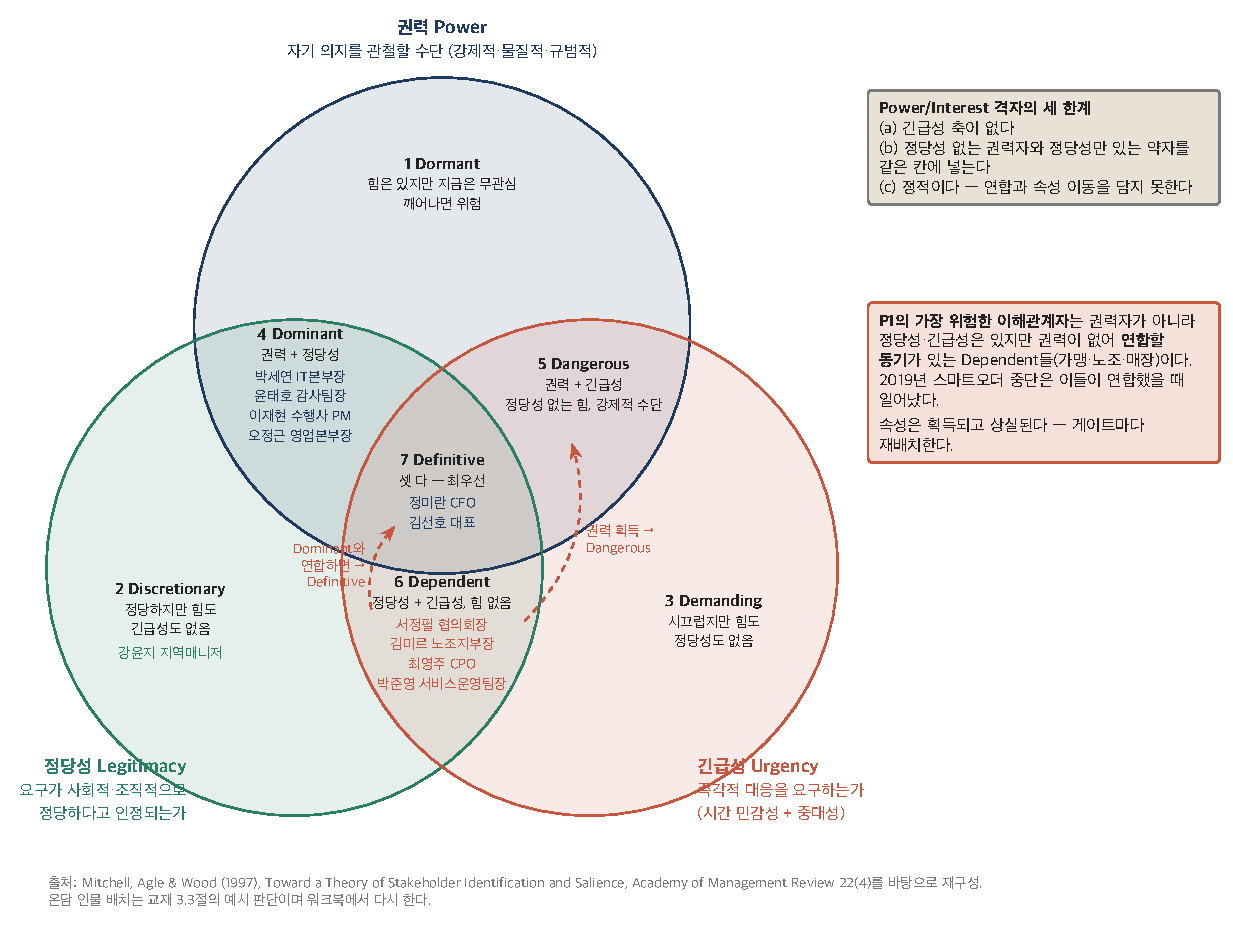
\includegraphics[width=1.00\textwidth,height=0.72\textheight,keepaspectratio]{../그림/PM_Day1/fig_3_3_salience.pdf}
\par\nobreak\vspace{1pt}{\scriptsize\color{mDarkTeal!70}그림 3-4. Mitchell-Agle-Wood 3속성 벤 다이어그램 7유형 + 온담 인물\par}
\end{center}
\framebreak
\begin{itemize}
\item\relax \textbf{권력(Power)} — 자기 의지를 관철할 수단 / \textbf{정당성(Legitimacy)} — 그 요구가 조직·사회적으로 정당한가 / \textbf{긴급성(Urgency)} — 즉각 대응을 요구하는가
\end{itemize}
{\usebeamercolor[fg]{normal text}\footnotesize\setlength{\tabcolsep}{3pt}\renewcommand{\arraystretch}{1.12}
\begin{tabular}{@{}>{\raggedright\arraybackslash}p{0.140\textwidth}>{\raggedright\arraybackslash}p{0.206\textwidth}>{\raggedright\arraybackslash}p{0.140\textwidth}>{\raggedright\arraybackslash}p{0.499\textwidth}@{}}
\toprule
\textbf{속성 수} & \textbf{유형} & \textbf{속성} & \textbf{의미} \\
\midrule
1 (잠재적) & Dormant 휴면 & P & 힘은 있지만 무관심. 깨어나면 위험 \\
 & Discretionary 재량 & L & 정당하지만 힘도 긴급성도 없음 \\
 & Demanding 요구 & U & 시끄럽지만 힘도 정당성도 없음 \\
2 (기대적) & Dominant 지배 & P+L & 전형적 핵심 이해관계자 \\
 & \textbf{Dangerous 위험} & \textbf{P+U} & 정당성 없는 힘 + 급함. 강제적 수단 사용 가능 \\
 & \textbf{Dependent 의존} & \textbf{L+U} & 정당하고 급하지만 힘이 없음 $\rightarrow$ 다른 이해관계자에 의존 \\
3 (확정적) & Definitive 확정 & P+L+U & 최우선 \\
\bottomrule
\end{tabular}}
\par\smallskip
\begin{itemize}
\item\relax 실무 가치 ①: \textbf{속성은 고정되어 있지 않다} — Dormant가 긴급성을 얻으면 Dangerous, Dependent가 Dominant와 연합하면 Definitive
\item\relax 실무 가치 ②: \textbf{유형마다 대응이 다르다} — Dangerous에게는 정당성을 부여(테이블에 앉힌다)하거나 권력을 차단, Dependent에게는 그를 대변할 Dominant를 찾아 준다
\end{itemize}
\note{§3.3 "Mitchell-Agle-Wood". 워크북 §3은 2$\times$2 대신 이 모델을 쓴다. 7유형 이름을 한국어·영어로 함께 익히게 한다 — 등록부 열 이름이다. 예상 소요 7분.}
\end{frame}

% ---- md slide 46: 온담의 이해관계자를 이 모델로 읽기 — 가장 위험한 사람은 권력자가 아니다
\begin{frame}[allowframebreaks=1.0]{온담의 이해관계자를 이 모델로 읽기 — 가장 위험한 사람은 권력자가 아니다}
\small
{\usebeamercolor[fg]{normal text}\footnotesize\setlength{\tabcolsep}{3pt}\renewcommand{\arraystretch}{1.12}
\begin{tabular}{@{}>{\raggedright\arraybackslash}p{0.110\textwidth}>{\raggedright\arraybackslash}p{0.245\textwidth}>{\raggedright\arraybackslash}p{0.118\textwidth}>{\raggedright\arraybackslash}p{0.130\textwidth}>{\raggedright\arraybackslash}p{0.170\textwidth}>{\raggedright\arraybackslash}p{0.212\textwidth}@{}}
\toprule
\textbf{인물} & \textbf{P} & \textbf{L} & \textbf{U} & \textbf{유형 (G0)} & \textbf{이동} \\
\midrule
정미란 CFO & 스폰서, 관리예비비 결재 & 이사회 조건 & 148억 집행 요구 & \textbf{Definitive} &  \\
김선호 대표 & 이사회 의장 & ○ & IPO 시계 & Definitive (일상은 Dormant처럼) & 게이트에서 깨어난다 \\
오정근 영업본부장 & Senior User, 가맹 협상 & 요구사항 대표 & 성수기·가맹 반발 시 급등 & Dominant & $\rightarrow$ Definitive \\
박세연 IT본부장 & 아키텍처 승인, \textbf{기존 시스템의 유일한 해독자} & ○ &  & Dominant & 권력의 원천은 직위가 아니라 지식 \\
한동석 물류본부장 & 3PL 계약 소관 & ○ & P1 관심 낮음 & Dominant & P2·WMS 연동에서 Definitive \\
\bottomrule
\end{tabular}}
\par\smallskip
\framebreak
{\usebeamercolor[fg]{normal text}\footnotesize\setlength{\tabcolsep}{3pt}\renewcommand{\arraystretch}{1.12}
\begin{tabular}{@{}>{\raggedright\arraybackslash}p{0.110\textwidth}>{\raggedright\arraybackslash}p{0.245\textwidth}>{\raggedright\arraybackslash}p{0.118\textwidth}>{\raggedright\arraybackslash}p{0.130\textwidth}>{\raggedright\arraybackslash}p{0.170\textwidth}>{\raggedright\arraybackslash}p{0.212\textwidth}@{}}
\toprule
\textbf{인물} & \textbf{P} & \textbf{L} & \textbf{U} & \textbf{유형 (G0)} & \textbf{이동} \\
\midrule
서정필 협의회장 & 388점 서면 동의 거부라는 \textbf{집합적} 권력 & 388점 대표, 데이터 소유 & 단말·데이터 결정 전 & \textbf{Dependent} & 오정근과 연합 시 Definitive \\
김미르 노조 지부장 & 현장 협조 거부 & 246명 대표 & 처리량 목표 공개 & Dependent & $\rightarrow$ \textbf{Dangerous} 가능 \\
최영주 CPO & "검토 의견만, 결정 안 함" & 규제 해석 & 2026-09-11 & Dependent & 박세연이 움직여야 \\
강윤지 지역매니저 & 없음 & 매장 현장 & 오픈 후 & Discretionary & 슈퍼유저 124명 대표가 되면 활용률 좌우 \\
\bottomrule
\end{tabular}}
\par\smallskip
\begin{itemize}
\item\relax 보이는 것: P1의 가장 위험한 이해관계자는 권력자가 아니라 \textbf{정당성과 긴급성은 있지만 권력이 없어 연합할 동기가 있는 사람들}(서정필·김미르·강윤지). \textbf{2019년의 실패는 이들이 연합했을 때 일어났다}
\end{itemize}
\note{§3.3 "온담의 이해관계자를 이 모델로 읽기". 판단은 예시이며 워크북 §3에서 25행으로 다시 한다. 윤태호 감사팀장(Dominant), 이재현 수행사 PM(Dominant, 61명·변경대가 청구권), 박준영(Dependent $\rightarrow$ 종료 시 Definitive)은 구두로. 생각해 볼 질문 4(서정필과 김미르가 연합하면 — 그 연합을 막는 것이 PM의 일인가, 정당한 것으로 테이블에 올리는 것이 PM의 일인가). 예상 소요 8분.}
\end{frame}

% ---- md slide 47: 한국 조직 특유의 이해관계자 넷 + 참여 계획
\begin{frame}[allowframebreaks=1.0]{한국 조직 특유의 이해관계자 넷 + 참여 계획}
\small
\par\smallskip\noindent{\usebeamercolor[fg]{normal text}\textbf{서구 문헌에 잘 안 나오지만 한국에서 반복적으로 결정적인}\par}\nobreak
\begin{itemize}
\item\relax \textbf{노동조합} — 시스템 도입은 노동 조건 변경, 단체협약상 사전 협의 대상일 수 있음. 인력 효율이 편익로 명시된 프로그램(매장 인건비율 21.4$\rightarrow$20.1\%, 물류 처리량)에서 착수부터 Definitive에 가까움. "P1은 인력 프로젝트가 아니다"는 맞지만 \textbf{노조가 그렇게 보지 않는다는 사실이 리스크}
\item\relax \textbf{가맹점주협의회} — 가맹사업법상 협의 의무, 부속서 개정은 개별 서면 동의. 가맹 판매 데이터와 단말은 가맹점주 소유 — 본사가 "우리 시스템"이라 부르는 것의 절반은 본사 것이 아니다
\item\relax \textbf{감사실 / 준법} — 과거 지적사항의 작성자이자 종료 후 감사의 수행자. 착수 시점에 "어떤 문서가 있으면 지적하지 않을 것인가"를 물어 두면 종료 비용이 준다
\item\relax \textbf{그룹 지주사 / 별도 법인} — ㈜온담푸드시스템은 100\% 종속이지만 별도 법인 $\rightarrow$ 계약 주체 둘, 개인정보 처리자 둘, 보안 정책 둘
\end{itemize}
\par\smallskip\noindent{\usebeamercolor[fg]{normal text}\textbf{참여 계획 — 분석은 대응이 있어야 의미가 있다}\par}\nobreak
\begin{itemize}
\item\relax 등록부 마지막 열: 현재 참여 수준 $\rightarrow$ 목표 수준 $\rightarrow$ 간극을 메울 \textbf{행동} (unaware / resistant / neutral / supportive / leading)
\item\relax 서정필: "발주 포털은 환영, 데이터·단말은 저항" $\rightarrow$ 한 사람을 두 행으로. 목표 "데이터 연동에 neutral 이상". 행동: 배포 범위·연동 수준을 동결 전에 \textbf{오정근을 통해} 협의회에 제시, 2026-08-14 이전
\item\relax \textbf{행동에 이름과 날짜가 없는 참여 계획은 계획이 아니다}
\end{itemize}
\note{§3.3 "한국 조직 특유의 이해관계자", "참여 계획", "실무에서 어떻게 틀리는가". 오류 넷: 착수 때 한 번 만들고 갱신 안 함(현저성은 게이트마다 재배치) / 직위만 적고 사람을 안 적음("오정근, 2005년 입사, 가맹사업팀장 출신, 재계약률 91\% KPI, 2019 스마트오더 중단을 겪음") / 부정적 이해관계자를 등록부에서 뺌 / PM 혼자 관리 — 서정필은 오정근이, 김미르는 한동석이, 윤태호는 정미란이. 예상 소요 7분.}
\end{frame}

% ---- md slide 48: 3교시 핵심 정리
\begin{frame}[allowframebreaks=1.0]{3교시 핵심 정리}
\small
\begin{enumerate}
\item\relax 착수의 첫 번째 일은 새로 만드는 것이 아니라 \textbf{이미 만들어진 비즈니스 케이스의 숫자와 가정을 검증}하고 결함을 목록으로 만들어 스폰서에게 결정을 요구하는 것
\item\relax \textbf{산출물은 PM의 책임, 활용·성과는 사업 오너의 책임}(ITO). 편익 오너를 PM으로 지정하면 범위 방어와 책임 회피가 합리적 행동이 된다. 편익 오너는 \textbf{상설 조직의 실명}
\item\relax 편익은 기술이 아니라 조직 변화에서 나온다(BDN). P1이 성공해도 편익이 안 나올 경로가 착수 시점에 보여야 한다
\item\relax 헌장은 계획서가 아니라 \textbf{권한 문서}. 목적에 솔루션을 적지 말고, 제외 범위·예산 층·가정·PM 권한(허용범위)을 채우며, 스폰서가 결정해야 할 빈칸(우선순위)을 남겨 결정을 요구한다
\item\relax Power/Interest는 긴급성과 정당성을 못 잡는다. 3속성·7유형으로 보면 P1의 가장 위험한 이해관계자는 권력자가 아니라 \textbf{연합할 동기가 있는 Dependent들}. 한국 특유의 넷 — 노조·가맹점주협의회·감사실·별도 법인
\end{enumerate}
\note{제3장 핵심 정리 1\textasciitilde{}5. 다음 교시가 바로 실습 ①(워크북 §1 비즈니스 케이스 요약, §2 헌장)이므로 워크북과 온담 정본을 준비시킨다. 예상 소요 3분.}
\end{frame}

\section{4교시 (90분) — 실습 ①: 온담 P1 비즈니스 케이스 요약 + 프로젝트 헌장}

% ---- md slide 49: 이 교시에서 하는 것
\begin{frame}[allowframebreaks=1.0]{이 교시에서 하는 것}
\small
\begin{itemize}
\item\relax \textbf{산출물 ① 비즈니스 케이스 요약} (Business Case Summary) — 워크북 §1. 약 35분
\par\nobreak
\begin{itemize}
\item\relax 이사회 승인본에서 P1 몫만 발라내고, 각 숫자의 \textbf{분모와 책임자}를 PM의 눈으로 확인한 두 쪽짜리 문서
\end{itemize}
\item\relax \textbf{산출물 ② 프로젝트 헌장} (Project Charter) — 워크북 §2. 약 50분
\par\nobreak
\begin{itemize}
\item\relax 15개 항목 중 \textbf{목적·성공 기준·범위/제외·예산 층·가정/제약·PM 권한·우선순위·완료 기준}에 집중
\end{itemize}
\item\relax 진행 방식: 각 산출물마다 과제 지시 $\rightarrow$ 작성 요령 $\rightarrow$ 흔한 오류 점검 $\rightarrow$ 완성 예시본과 대조
\item\relax 준비물: 워크북 §0.3 온담 한 페이지 요약, §1.4·§2.4 빈 템플릿, §1.5·§2.5 완성 예시본
\item\relax 3\textasciitilde{}7년차: 각 절의 \textbf{심화 과제}(자기 회사 프로젝트로 같은 문서)를 병행
\end{itemize}
\note{워크북 §0.1 사용법 — X.3 항목별 가이드가 가장 중요하고 X.5 완성 예시본이 그 다음. 예시본은 "정답"이 아니라 "판단의 흔적이 보이는 문서"라고 말해 둔다. 숫자에는 값·단위·출처(C-01, O-08 같은 정본 ID)를 붙이는 습관. 예상 소요 3분.}
\end{frame}

% ---- md slide 50: 산출물 ① 비즈니스 케이스 요약 — 과제 지시
\begin{frame}[allowframebreaks=1.0]{산출물 ① 비즈니스 케이스 요약 — 과제 지시}
\small
\begin{itemize}
\item\relax \textbf{과제}: 워크북 §1.4 빈 템플릿의 9개 항목 중 \textbf{항목 2(전략적 배경) · 항목 4(편익) · 항목 6(재무 평가) · 항목 9(편익 책임자)}를 온담 P1로 채우라. 나머지 항목은 §1.5 예시본을 읽고 확인
\item\relax \textbf{왜 PM이 다시 쓰는가} (워크북 §1.1)
\par\nobreak
\begin{itemize}
\item\relax 승인 문서의 숫자를 PM이 검산하지 않으면 그 숫자는 나중에 \textbf{PM의 약속}이 된다 — 214억 안의 "물류 96억"은 P2의 설비가 만드는 숫자
\item\relax 비즈니스 케이스는 게이트마다 갱신되는 살아 있는 문서(PRINCE2 continued business justification) — 갱신 기준선이 없으면 중단 결정을 못 내리는 좀비
\end{itemize}
\item\relax \textbf{분야별 무게} (워크북 §1.1): SI는 수행사 PM이 발주사 BC를 본 적조차 없는 경우가 많다 / EPC는 FEL $\rightarrow$ FID에서 AACE Class 3 이상과 함께 고정 / NPD는 게이트 문서 자체가 BC이며 매 게이트 갱신. \textbf{한 번 쓰고 끝내는 분야는 IT뿐}
\item\relax 표준 위치: PMBOK 8판 Governance·Initiating의 입력 문서 / 6판 1.2.6·4.1 입력 / PRINCE2 Outline BC $\rightarrow$ BC $\rightarrow$ 단계마다 갱신 / ISO 21502 §6.2·§7.3 / (참고) Green Book Five Case Model
\end{itemize}
\note{워크북 §1.1\textasciitilde{}1.2. 시간이 부족하면 항목 4(편익)와 항목 9(책임자)만 완성시킨다 — 이 둘이 헌장 성공 기준의 입력이다. 예상 소요 5분.}
\end{frame}

% ---- md slide 51: 작성 요령 ① — 전략적 배경 · 대안 · 편익 (워크북 §1.3 항목 2~4)
\begin{frame}[allowframebreaks=1.0]{작성 요령 ① — 전략적 배경 · 대안 · 편익 (워크북 §1.3 항목 2\textasciitilde{}4)}
\small
\par\smallskip\noindent{\usebeamercolor[fg]{normal text}\textbf{항목 2 전략적 배경 — "왜 지금인가"}\par}\nobreak
\begin{itemize}
\item\relax 3\textasciitilde{}5문단, 문단마다 숫자 하나 이상. 현재 상태를 측정값으로(폐기율 3.9\%), \textbf{분모}를 밝히고(취급원가 2,530억), \textbf{do-nothing 시나리오를 한 문단 이상}
\item\relax 온담: 세 압력 — 기술 부채 한계(OD-POS OS 종료 2024-07, SAP ECC 2027-12) / IPO 시계(2027 3분기 예비심사) / 규제 시행일(2026-09-11, 2027-03-31) + 두 번의 실패 이력. do-nothing = "OS 지원 종료 상태로 615개 매장 결제를 계속 처리한다"
\end{itemize}
\par\smallskip\noindent{\usebeamercolor[fg]{normal text}\textbf{항목 3 대안 검토} — 최소 셋(do-nothing / do-minimum / 제안안) + 기각된 대안 하나 이상. 기각 사유 한 줄이라도 반드시\par}\nobreak
\begin{itemize}
\item\relax 온담: ① 현행 유지 ② do-minimum(OS 마이그레이션 + 인터페이스 문서화, 약 18억 [추가 설정]) ③ 상용 리테일 패키지 — 기각: 가맹·B2B·직영 세 모델을 한 패키지가 못 다루고 SAP 병행 요건 미충족 ④ 제안안 168억
\end{itemize}
\par\smallskip\noindent{\usebeamercolor[fg]{normal text}\textbf{항목 4 편익} — 항목별 기준값·목표값·시점·연간 금액·\textbf{산출 분모}·\textbf{측정 책임자}. \textbf{분모 열과 책임자 열이 없는 편익 표는 편익 표가 아니다}\par}\nobreak
\begin{itemize}
\item\relax P1 직접 기여(폐기율 43, 배달수수료 회피 37, 매장 인건비율 38 = \textbf{118억}, 리드타임·재고 정확도·결품률)와 P2 의존(물류 96억)을 \textbf{분리}. 운영비 27억 미차감 명시. 재고 정확도 91.3\%의 분모(순환실사 SKU 69\%)를 주석으로
\end{itemize}
\note{워크북 §1.3 항목 2\textasciitilde{}4. 항목 4에서 "P1 편익을 118억으로 한정"하는 결정이 이 문서의 핵심 판단 — §1.6 해설 "편익을 정직하게 나누는 것은 겸손이 아니라 자기 방어이며 프로그램 전체의 편익 관리를 가능하게 하는 유일한 방법". 예상 소요 8분.}
\end{frame}

% ---- md slide 52: 작성 요령 ② — 비용 · 재무 평가 · 편익 책임자 (워크북 §1.3 항목 5~6, 9)
\begin{frame}[allowframebreaks=1.0]{작성 요령 ② — 비용 · 재무 평가 · 편익 책임자 (워크북 §1.3 항목 5\textasciitilde{}6, 9)}
\small
\par\smallskip\noindent{\usebeamercolor[fg]{normal text}\textbf{항목 5 비용} — 구축(8개 항목 내역)과 운영(연 27억 $\times$ 3년 = 81억)을 구분, 3층 구조(168.0 / 156.0 / 145.8)의 정의를 밝히고 5년 TCO 한 줄\par}\nobreak
\begin{itemize}
\item\relax 흔한 오류: "SI 개발비 68.2억"만 적어 예산이 실제의 40\%로 보이는 것 / 운영비 누락 / 예비비를 빼고 "예산 안에 맞췄다"
\end{itemize}
\par\smallskip\noindent{\usebeamercolor[fg]{normal text}\textbf{항목 6 재무 평가} — 편익과 비용을 같은 시간축에. 할인율과 실현 기간 명시. \textbf{편익이 몇 \% 실현되어야 손익분기인가}가 NPV보다 의사결정자에게 유용\par}\nobreak
\begin{itemize}
\item\relax 예시본(§1.5, 계산은 [추가 설정]): 회수기간 착수 기준 약 3.4년 / NPV(8\%, 5년) 약 +134억 / 민감도 100\%: +134, 70\%: 약 +16, 50\%: 약 $-$63 / \textbf{손익분기 편익 실현률 약 66\%} (118억의 66\% $\approx$ 78억이 M+24부터 매년)
\item\relax 이사회의 관심은 IRR이 아니라 "부채비율 187\%인 회사가 1차연도에 얼마를 쓰는가" $\rightarrow$ 연차별 현금 유출을 함께
\end{itemize}
\par\smallskip\noindent{\usebeamercolor[fg]{normal text}\textbf{항목 9 편익 책임자와 검토 일정} — 부서명이 아니라 \textbf{직책과 실명}. 검토 시점은 종료 후(M+12 2027-01, G5 2028-03-31)\par}\nobreak
\begin{itemize}
\item\relax 폐기율·결품률·인건비율: 오정근 / 재고 정확도: 한동석(분모 확장은 나영선과 협의) / 온라인·배달수수료: 오정근 [추가 설정]
\item\relax \textbf{PM은 한 명도 없다} — G5에 PM은 그 자리에 없다. 이 표에 서명을 받는 것이 헌장 서명보다 어렵고, 그래서 더 중요하다
\end{itemize}
\note{워크북 §1.3 항목 5·6·9와 §1.6 해설. 66\%라는 숫자가 헌장 항목 14 조기 종료 조건("G1·G2에서 손익분기 66\% 미달 전망 시 중단 부의")으로 흘러간다는 점을 미리 말한다. 운영비 27억 전액을 P1에 귀속한 것은 보수적 검산이라는 §1.6 해설도 한 줄. 예상 소요 8분.}
\end{frame}

% ---- md slide 53: 산출물 ① 흔한 오류 점검 + 예시본 참조
\begin{frame}[allowframebreaks=1.0]{산출물 ① 흔한 오류 점검 + 예시본 참조}
\small
\par\smallskip\noindent{\usebeamercolor[fg]{normal text}\textbf{흔한 오류 체크리스트} (워크북 §1.3 각 항목의 "흔한 오류" 칸)\par}\nobreak
\begin{itemize}
\item[$\square$]\relax 원본 승인 문서(2025-12 이사회 부의안)를 적지 않아 요약본이 독립 문서처럼 돌아다닌다
\item[$\square$]\relax 솔루션을 배경으로 적었다 ("클라우드 POS가 필요하다") / 형용사만 있고 숫자가 없다 ("노후화가 심각하다")
\item[$\square$]\relax 제안안 하나만 적고 "대안 없음" — 검토가 아니라 사후 정당화 / 대안 간 비교 기준이 다르다
\item[$\square$]\relax 214억을 그대로 옮기고 분모를 확인하지 않았다 / 다른 프로젝트 편익을 자기 것으로 / 측정 책임자 "추후 지정"
\item[$\square$]\relax 편익 100\% 실현을 전제로 IRR 40\%를 제시했다 / 할인율이 없다 / 편익 실현 시점을 종료 직후로
\item[$\square$]\relax 리스크 칸에 "일정 지연", "요구사항 변경" 같은 일반론
\item[$\square$]\relax 이사회 승인 조건 5개를 요약본에서 빠뜨렸다 / 다음 갱신 시점(G1 2026-04-30)이 없다
\end{itemize}
\par\smallskip\noindent{\usebeamercolor[fg]{normal text}\textbf{예시본과 대조할 것} (워크북 §1.5\textasciitilde{}1.6)\par}\nobreak
\begin{itemize}
\item\relax 왜 P1 편익을 118억으로 한정했는가 / 왜 do-minimum을 G1까지 폴백으로 남겼는가(예산 삭감이 곧 중단이 된 2019년의 결말) / 왜 손익분기 66\%를 굳이 계산했는가 / 왜 재고 정확도 분모 문제를 별도 항목으로
\end{itemize}
\par\smallskip\noindent{\usebeamercolor[fg]{normal text}\textbf{점검 질문} (§1.7): 편익 표 모든 행에 분모와 실명이 있는가 / 손익분기 실현률을 한 문장으로 말할 수 있는가 / do-nothing 비용이 0으로 적혀 있지 않은가\par}\nobreak
\note{15분 작성 후 5분 예시본 대조. §1.7 기본 과제(CFO 148억 확정, P1 2026년 집행 102$\rightarrow$86억 시 항목 5·6 재작성)는 시간이 남는 조에만. 예상 소요 5분 (설명) + 작성 시간.}
\end{frame}

% ---- md slide 54: 산출물 ② 프로젝트 헌장 — 과제 지시
\begin{frame}[allowframebreaks=1.0]{산출물 ② 프로젝트 헌장 — 과제 지시}
\small
\begin{itemize}
\item\relax \textbf{과제}: 워크북 §2.4 빈 템플릿 15개 항목 중 \textbf{항목 2(목적) · 3(성공 기준) · 5(범위/제외) · 8(예산) · 9(가정/제약) · 12(거버넌스·PM 권한) · 13(우선순위) · 14(완료 기준)}을 온담 P1로 채우라. 나머지 7개는 §2.5 예시본을 읽고 확인
\item\relax 헌장이 답하는 질문은 여섯 개뿐 (워크북 §2.1): \textbf{왜 하는가 / 무엇이 성공인가 / 어디까지가 범위인가 / 누가 결정하는가 / PM은 무엇을 혼자 결정할 수 있는가 / 언제 끝난 것으로 보는가}
\item\relax 없거나 형식적일 때 터지는 것: \textbf{범위 경계 분쟁}("가맹점 단말 교체 비용은 누가 내는가" $\rightarrow$ 동결 직전 주에 388점 반발과 함께 돌아온다) / \textbf{PM 권한의 공백}(전결 5억 vs 허용범위 10.08억) / \textbf{성공 기준 부재}(2019 스마트오더는 "중단"이 실패인지 손절인지조차 판정 못 함 $\rightarrow$ 감사 지적 "손실 확정 절차 부재")
\item\relax 분야별 실체 (워크북 §2.1): SI는 발주사 헌장 vs 수행사 착수계·사업수행계획서의 간극이 변경대가 분쟁의 씨앗 / EPC는 FID 문서 + PEP, "제약" 칸이 LD·성능 보증·준공 기한으로 훨씬 무겁다 / NPD는 게이트 통과 문서, 시장 진입 시점과 target cost가 성공 기준
\item\relax 어느 분야든 가장 중요한 칸은 "무엇을 만드는가"가 아니라 \textbf{"무엇을 만들지 않는가"와 "누가 무엇을 결정하는가"}
\end{itemize}
\note{워크북 §2.1\textasciitilde{}2.2. PM이 초안을 쓰고 스폰서가 서명하는 순서가 헌장을 왜곡한다(PM은 자기 권한을 넓게 쓰기 어렵고 스폰서는 자기 책임을 좁게 읽는다) $\rightarrow$ 그래서 가장 협상이 필요한 칸이 항목 12. 예상 소요 5분.}
\end{frame}

% ---- md slide 55: 작성 요령 ③ — 목적 · 성공 기준 · 범위/제외 (워크북 §2.3 항목 2·3·5)
\begin{frame}[allowframebreaks=1.0]{작성 요령 ③ — 목적 · 성공 기준 · 범위/제외 (워크북 §2.3 항목 2·3·5)}
\small
\par\smallskip\noindent{\usebeamercolor[fg]{normal text}\textbf{항목 2 목적} — 3\textasciitilde{}5문장, 숫자 필수, 편익 문서 ID 인용. §1 결론을 인용하되 다시 쓰지 않는다\par}\nobreak
\begin{itemize}
\item\relax 온담: "615개 매장·물류센터·공장의 주문과 재고를 하나의 원장으로 실시간 관리할 수 있게 하여 폐기율 3.9\%$\rightarrow$2.2\%, 결품률 4.7\%$\rightarrow$1.5\%, 가맹 발주 리드타임 38h$\rightarrow$12h를 달성하고(연 직접 편익 118억), 지원 종료된 OD-POS를 규제 기한(2026-09-11, 2027-03-31) 안에 대체한다"
\item\relax 오류: "플랫폼을 구축한다"(수단) / 프로그램 전체의 목적을 그대로 (P1 $\neq$ ONE ONDAM)
\end{itemize}
\par\smallskip\noindent{\usebeamercolor[fg]{normal text}\textbf{항목 3 성공 기준} — 표: 목표 / 지표 / 목표값 / \textbf{판정 시점} / \textbf{판정자}. 두 층\par}\nobreak
\begin{itemize}
\item\relax 관리 성공(G4): 2027-05-29 이내(+15영업일), 156억 이내(+6\%), RTM 커버리지 100\%, 결함밀도 0.4건/FP 이하, SAC 미해소 0건
\item\relax 프로젝트 성공(G5): M+12 리드타임 12h, M+24 폐기율 2.2\% 등 — §1 편익 표 인용
\item\relax 오류: "안정적으로 가동한다" / 판정자·시점 없음 / 편익 목표를 G4에 판정
\end{itemize}
\par\smallskip\noindent{\usebeamercolor[fg]{normal text}\textbf{항목 5 범위 — 포함 / 제외 / 경계 조건} — 제외를 포함과 \textbf{같은 무게, 같은 분량}으로. 각 제외 항목에 \textbf{그러면 누가 하는가}\par}\nobreak
\begin{itemize}
\item\relax 포함 5개 산출물. 제외: SAP ECC 교체, 설비·WMS(P2), 교육·가맹 계약 개정(P3), 규제 등록(P4), 운영 조직(P5), \textbf{가맹점 단말 하드웨어 교체}
\item\relax 경계: 가맹 단말은 기존 HW에 SW 배포까지 / 3PL WMS 연동 명세는 작성하되 계약 변경 협상은 물류본부
\item\relax 오류: "기타 부대 업무 일체"(수행사는 무한 범위로, 발주사는 무상 서비스로 읽는다)
\end{itemize}
\note{워크북 §2.3 항목 2·3·5. 항목 4(상위 요구사항 5\textasciitilde{}10줄, 요구 제공자 괄호), 6(산출물 — 소스·형상 인수, 운영 문서 포함; 2023 감사 지적), 7(마일스톤 — 외부 고정 날짜 굵게)은 구두로 한 줄씩. §2.6 해설 "왜 제외 범위에 가맹점 단말 HW를 굵게 넣었는가" — 헌장에서 가장 논쟁적인 줄이고 그래서 가장 필요한 줄. 예상 소요 8분.}
\end{frame}

% ---- md slide 56: 작성 요령 ④ — 예산 층 · 가정/제약 · PM 권한 · 우선순위 · 완료 기준 (항목 8·9·12·13·14)
\begin{frame}[allowframebreaks=1.0]{작성 요령 ④ — 예산 층 · 가정/제약 · PM 권한 · 우선순위 · 완료 기준 (항목 8·9·12·13·14)}
\small
\par\smallskip\noindent{\usebeamercolor[fg]{normal text}\textbf{항목 8 예산} — 3층 표 + 컨틴전시(PM 통제 10.2억, 단 5,000만 원 이상 단일 건은 CFO 결재 지침 적용)와 관리예비비(스폰서 12.0억) 구분. 위임전결과의 관계 한 줄\par}\nobreak
\par\smallskip\noindent{\usebeamercolor[fg]{normal text}\textbf{항목 9 가정 / 제약} — 각 5\textasciitilde{}10줄. 가정에 \textbf{확인 시점·확인 책임자}, 제약에 \textbf{출처}\par}\nobreak
\begin{itemize}
\item\relax 가정: 3PL 계약 변경 2026-06 타결(한동석) / 가맹 부속서 2026-08-14(오정근) / 겸임 14명 투입률 50\% 이상(박세연)
\item\relax 제약: 성수기 변경 금지 창 / 규제 기한 2개 / 컷오버 창 / 본부장 전결 5억 / OD-POS·SAP 병행 / 자사앱 소스 벤더 보유
\item\relax 오류: 가정이 희망사항("충분한 인력이 확보된다") / 제약에 자기 팀이 정한 것
\end{itemize}
\par\smallskip\noindent{\usebeamercolor[fg]{normal text}\textbf{항목 12 거버넌스·PM 권한} — 허용범위 표(원가 +6\% / 일정 +15영업일 / 범위 $\pm$3\% / 품질 0.4건/FP / 리스크 EMV 8억 / 편익 $-$5\%p) + 에스컬레이션 3단계 + \textbf{"PM은 이 범위 안에서 스폰서 보고 없이 결정한다"} 문장 + 전결 충돌 처리("허용범위 내라도 5억 초과 건은 CFO 결재 병행")\par}\nobreak
\par\smallskip\noindent{\usebeamercolor[fg]{normal text}\textbf{항목 13 우선순위} — 고정 / 조정 가능 / 수용 세 칸, 이유 한 문장. \textbf{스폰서가 결정해 적는다}\par}\nobreak
\begin{itemize}
\item\relax 대표는 일정, CFO는 원가, 수행사는 범위를 고정하려 한다 $\rightarrow$ 세 개를 다 고정하면 조정 변수는 품질뿐 = 결함을 운영으로 넘긴다는 뜻
\item\relax 예시본: 컷오버 창 고정, 원가는 집행 한도 내 고정, \textbf{범위(SRS 570건 중 옴니채널 고도화)를 조정 변수로} — 그중 규제·가용성은 고정, 고도화는 이연 가능
\end{itemize}
\par\smallskip\noindent{\usebeamercolor[fg]{normal text}\textbf{항목 14 완료 기준} — 정상 종료(G4 SAC 미해소 0건 또는 해소 기한·책임자 서명, 판정 박준영·승인 정미란) + \textbf{조기 종료 조건}(G1·G2에서 손익분기 66\% 미달 전망 / 컷오버 창 2회 연속 이탈 $\rightarrow$ 스폰서가 이사회에 중단 부의, 손실 확정은 재경팀장)\par}\nobreak
\note{워크북 §2.3 항목 8·9·12·13·14. §2.6 해설의 두 문장을 반드시 — "초과가 \textbf{예상되는} 시점"이라는 단어 하나가 거버넌스가 작동하는지 장식인지를 가른다 / 중단은 실패가 아니다, 손익분기에 못 미칠 것이 확실한 프로젝트를 계속하는 것이 실패다(이사회 조건 5항에 대한 직접 답). 예상 소요 10분.}
\end{frame}

% ---- md slide 57: 산출물 ② 흔한 오류 점검 + 예시본 참조
\begin{frame}[allowframebreaks=1.0]{산출물 ② 흔한 오류 점검 + 예시본 참조}
\small
\par\smallskip\noindent{\usebeamercolor[fg]{normal text}\textbf{헌장의 여덟 가지 오류} (교재 §3.2) — 여러분 초안에 몇 개가 있는가\par}\nobreak
\begin{itemize}
\item[$\square$]\relax 킥오프 발표 자료로 대체 $\square$~ 목적 칸에 솔루션 $\square$~ 제외 범위 비움 $\square$~ 예산을 한 숫자로
\item[$\square$]\relax PM 권한을 "총괄"로 $\square$~ 편익 목표를 PM 성공 기준에 $\square$~ 가정을 안 적음 $\square$~ 스폰서가 읽지 않은 헌장에 서명
\item\relax 추가 (워크북 §2.3): 승인자 칸에 "경영진"·"운영위원회"(위원회는 서명하지 않는다) / 우선순위를 전부 "고정"으로(희망이지 우선순위가 아님) / 종료 조건이 없어 무한 하자보수 / Senior User 서명 없이 나중에 "우리는 동의한 적 없다"
\end{itemize}
\par\smallskip\noindent{\usebeamercolor[fg]{normal text}\textbf{예시본과 대조할 것} (워크북 §2.5\textasciitilde{}2.6)\par}\nobreak
\begin{itemize}
\item\relax 왜 제외 범위에 가맹점 단말 HW를 굵게 / 왜 성공 기준을 두 층으로 / 왜 우선순위에서 범위를 조정 변수로 / 왜 "초과가 예상되는 시점"이라고 썼는가 / 왜 허용범위 10.08억과 전결 5억의 충돌을 헌장에 적었는가 / 왜 조기 종료 조건에 손실 확정 절차까지
\end{itemize}
\par\smallskip\noindent{\usebeamercolor[fg]{normal text}\textbf{점검 질문} (§2.7)\par}\nobreak
\begin{enumerate}
\item\relax 목적 문단에 "구축한다", "도입한다"로 끝나는 문장이 있는가 $\rightarrow$ 뒤에 "그래서 무엇이 얼마나 좋아지는가"를 붙이라
\item\relax 제외 범위 각 항목 옆에 "그러면 누가 하는가"가 있는가
\item\relax \textbf{PM이 스폰서에게 묻지 않고 결정할 수 있는 금액과 기간을 한 문장으로 말할 수 있는가} — 말할 수 없다면 아직 권한 부여 문서가 아니다
\end{enumerate}
\note{25분 작성 후 10분 대조. 조별로 항목 13(우선순위) 결정을 발표시키면 대표·CFO·수행사의 세 시계가 조마다 다르게 해소되는 것이 보인다. 예상 소요 5분 (설명) + 작성 시간.}
\end{frame}

% ---- md slide 58: 4교시 정리 — 두 문서에서 반복된 규칙
\begin{frame}[allowframebreaks=1.0]{4교시 정리 — 두 문서에서 반복된 규칙}
\small
\begin{enumerate}
\item\relax \textbf{숫자에는 값·단위·출처·분모}가 붙는다. 214억이 아니라 "P1 직접 118억(43+37+38), 분모 취급원가 2,530억, 운영비 27억 미차감"
\item\relax \textbf{사람은 부서명이 아니라 직책·실명}이며, 편익 책임자는 PM이 아니다 — G5에 PM은 그 자리에 없다
\item\relax 헌장은 채워 넣는 문서가 아니라 \textbf{스폰서에게 결정을 요구하는 문서} — 우선순위·허용범위·편익 오너·미확정 가정
\item\relax \textbf{PM이 통제하지 못하는 것을 문서로 남기는 것}(가정·제약·제외 범위)이 PM의 권한을 지키는 방법
\item\relax 비즈니스 케이스의 66\%와 헌장의 조기 종료 조건은 한 줄로 이어진다 — 오늘 쓴 것은 G1(2026-04-30)에 v1.0$\rightarrow$v1.1로 확정되는 \textbf{초안}
\end{enumerate}
\note{워크북 §6 "공통 규칙" 세 가지를 앞당겨 말한다. 5교시는 헌장 항목 12(거버넌스·PM 권한)와 10(리스크)의 이론이다 — "방금 쓴 PM 권한 칸이 왜 그렇게 쓰기 어려웠는지"를 5교시가 설명한다고 연결. 예상 소요 3분.}
\end{frame}

\section{5교시 (75분) — 거버넌스 · 권한 없는 PM · 프리모템 · 분야별 착수 노하우}

% ---- md slide 59: 이 교시에서 배우는 것
\begin{frame}[allowframebreaks=1.0]{이 교시에서 배우는 것}
\small
\begin{itemize}
\item\relax 거버넌스 — 스폰서·운영위원회·PMO·PM의 권한 구조 [§3.4]
\par\nobreak
\begin{itemize}
\item\relax Manage by Exception과 허용범위 격자 / "권한 없는 PM"이 한국에서 왜 일반적이며 어떻게 일하는가
\end{itemize}
\item\relax 초기 리스크와 프리모템 [§3.5]
\par\nobreak
\begin{itemize}
\item\relax 착수 시점 리스크의 세 원천 / 계획 오류와 외부 시각 / Gary Klein의 프리모템
\end{itemize}
\item\relax 분야별 착수 노하우 — SI, 건설·EPC, 제조 NPD, 제약 [§3.6]
\item\relax 6교시 실습 ②(이해관계자 등록부·RACI·프리모템)의 이론 부분
\end{itemize}
\note{제3장 §3.4\textasciitilde{}3.6. 시간 배분: §3.4 25분, §3.5 22분, §3.6 20분, 정리 5분. 4교시에서 수강생이 헌장 항목 12를 쓰며 막혔던 지점("PM 권한을 무엇으로 채우나")이 §3.4의 출발점이다. 예상 소요 2분.}
\end{frame}

% ---- md slide 60: 거버넌스 — 조직도가 아니라 결정의 흐름
\begin{frame}[allowframebreaks=1.0]{거버넌스 — 조직도가 아니라 결정의 흐름}
\small
\begin{center}\usebeamercolor[fg]{normal text}
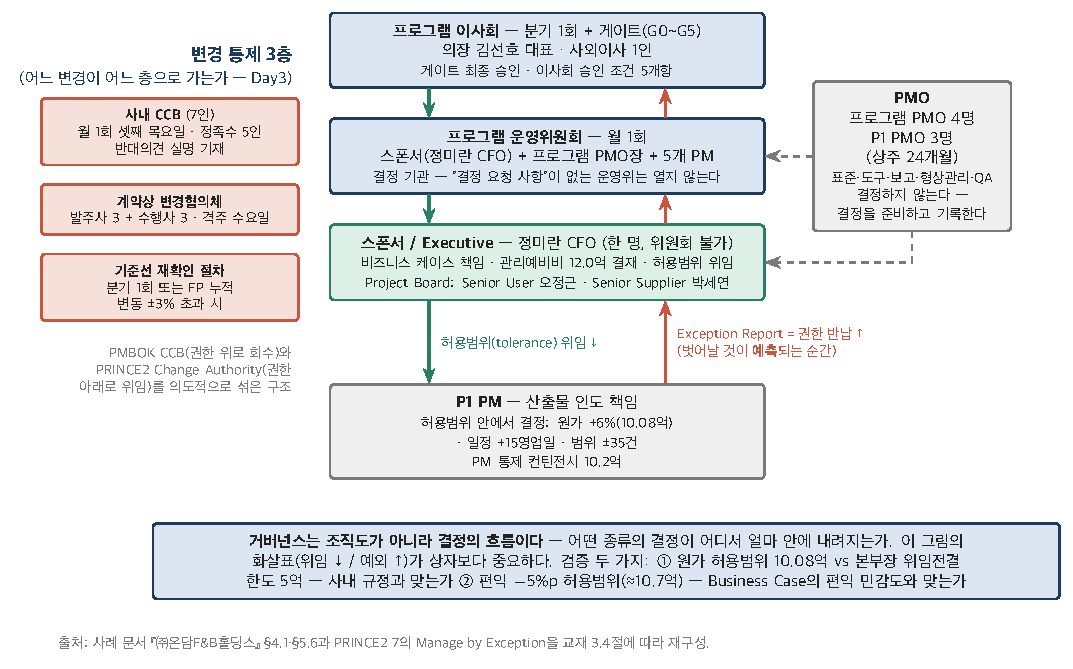
\includegraphics[width=1.00\textwidth,height=0.72\textheight,keepaspectratio]{../그림/PM_Day1/fig_3_4_governance.pdf}
\par\nobreak\vspace{1pt}{\scriptsize\color{mDarkTeal!70}그림 3-5. 온담 P1 거버넌스 — 결정의 흐름(위임↓/예외↑)과 변경 통제 3층\par}
\end{center}
\framebreak
\begin{itemize}
\item\relax 거버넌스 = \textbf{"누가 무엇을 결정하고 누구에게 책임지는가"의 구조}. PMBOK 8판 첫 도메인 / ISO 21505:2017 별도 표준 / PRINCE2 첫 프로세스 Directing a Project — 실패의 가장 흔한 원인은 기술이 아니라 \textbf{결정의 부재}
\end{itemize}
{\usebeamercolor[fg]{normal text}\footnotesize\setlength{\tabcolsep}{3pt}\renewcommand{\arraystretch}{1.12}
\begin{tabular}{@{}>{\raggedright\arraybackslash}p{0.134\textwidth}>{\raggedright\arraybackslash}p{0.331\textwidth}>{\raggedright\arraybackslash}p{0.520\textwidth}@{}}
\toprule
\textbf{구성 요소} & \textbf{원칙} & \textbf{온담 P1} \\
\midrule
\textbf{스폰서} (Executive) & 자원을 대고 BC에 책임. \textbf{한 명}. 위원회는 스폰서가 될 수 없다 & 정미란 CFO — 프로그램 스폰서 겸임(P1 별도 스폰서 없음) $\rightarrow$ 워크북 논점 \\
\textbf{운영위원회} (Steering / Board) & 스폰서가 의장인 결정 기관. \textbf{"결정 요청 사항"이 없는 운영위는 열지 않는 편이 낫다} & 프로그램 운영위(월 1회) + 프로그램 이사회(분기 + 게이트, 의장 김선호) 2층 \\
\textbf{PMO} & 표준·도구·보고·형상관리·QA 지원. \textbf{PMO는 결정하지 않는다 — 결정을 준비하고 기록한다} & 프로그램 PMO 4 + P1 PMO 3(상주 24개월, 12.6억) + P2 PMO 2 \\
\bottomrule
\end{tabular}}
\par\smallskip
\framebreak
{\usebeamercolor[fg]{normal text}\footnotesize\setlength{\tabcolsep}{3pt}\renewcommand{\arraystretch}{1.12}
\begin{tabular}{@{}>{\raggedright\arraybackslash}p{0.134\textwidth}>{\raggedright\arraybackslash}p{0.331\textwidth}>{\raggedright\arraybackslash}p{0.520\textwidth}@{}}
\toprule
\textbf{구성 요소} & \textbf{원칙} & \textbf{온담 P1} \\
\midrule
\textbf{PM} & 산출물 인도, 허용범위 안에서 결정, 벗어나면 에스컬레이션 &  \\
\textbf{변경 통제 기구} &  & \textbf{3층} — 사내 CCB(7인, 월 셋째 목요일, 정족수 5, 반대의견 실명) / 계약상 변경협의체(3+3, 격주 수요일) / 기준선 재확인(분기 또는 FP $\pm$3\%) $\rightarrow$ Day3 \\
\bottomrule
\end{tabular}}
\par\smallskip
\begin{itemize}
\item\relax 가장 근본적인 오류: 거버넌스를 "조직도 그리기"로 이해하는 것. \textbf{어떤 종류의 결정이 어디서 얼마 안에 내려지는지}가 그려져야 한다
\end{itemize}
\note{§3.4 "개념"과 "실무에서 어떻게 틀리는가". PMO가 결정하기 시작하면 스폰서가 결정하지 않게 된다. 생각해 볼 질문 2(P1 스폰서 = 프로그램 스폰서는 장점인가 단점인가). 예상 소요 6분.}
\end{frame}

% ---- md slide 61: Manage by Exception — 허용범위 격자 (온담 초안, 사례 §5.6)
\begin{frame}[allowframebreaks=1.0]{Manage by Exception — 허용범위 격자 (온담 초안, 사례 §5.6)}
\small
\begin{columns}[T,onlytextwidth]
\begin{column}{0.42\textwidth}
{\usebeamercolor[fg]{normal text}\scriptsize\setlength{\tabcolsep}{3pt}\renewcommand{\arraystretch}{1.12}
\begin{tabular}{@{}>{\raggedright\arraybackslash}p{0.217\linewidth}>{\raggedright\arraybackslash}p{0.259\linewidth}>{\raggedright\arraybackslash}p{0.292\linewidth}>{\raggedright\arraybackslash}p{0.217\linewidth}@{}}
\toprule
\textbf{축} & \textbf{작업패키지} & \textbf{\textbf{프로젝트 (P1)}} & \textbf{프로그램} \\
\midrule
원가 & +2\% & \textbf{+6\% (10.08억)} & +12\% \\
일정 & +5영업일 & \textbf{+15영업일} & +30영업일 \\
범위 & $\pm$1\% & \textbf{$\pm$3\% ($\pm$35건)} & $\pm$6\% \\
품질 & 결함밀도 0.13건/FP & \textbf{0.4건/FP} & 0.8건/FP \\
리스크 & EMV 2.7억 & \textbf{EMV 8억} & EMV 16억 \\
편익 & $-$1.7\%p & \textbf{$-$5\%p} & $-$10\%p \\
안전·지속가능성 & 0 & 0 & 0 \\
\bottomrule
\end{tabular}}
\par\smallskip
\end{column}\begin{column}{0.56\textwidth}
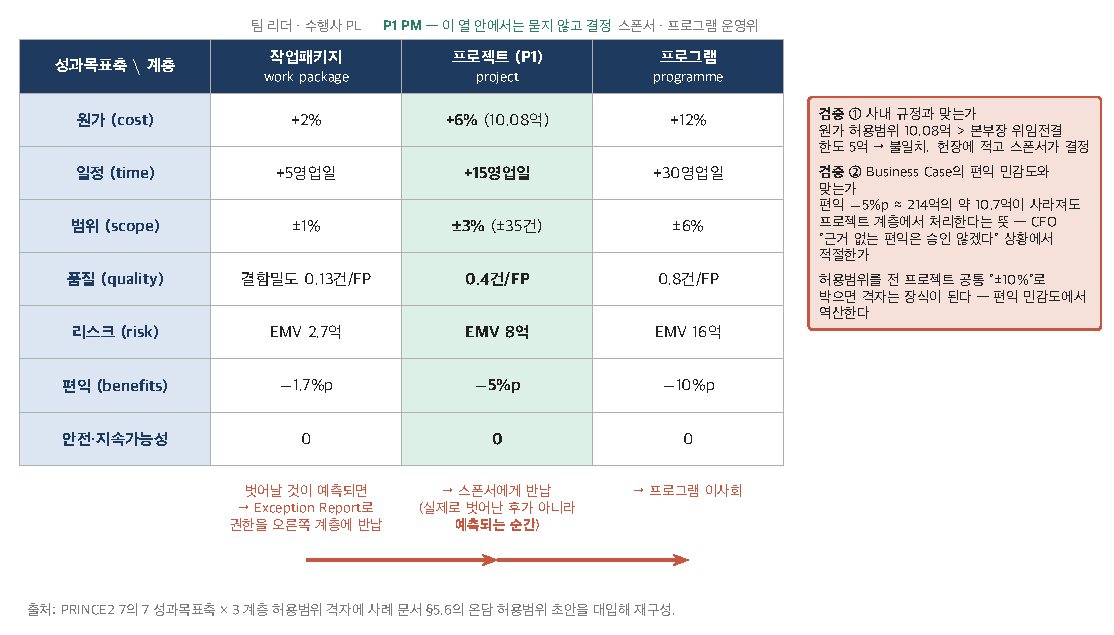
\includegraphics[width=\linewidth,height=0.8\textheight,keepaspectratio]{../그림/PM_Day1/fig_3_4_tolerance_grid.pdf}
\end{column}\end{columns}
\begin{itemize}
\item\relax 이 격자가 말하는 것: P1 PM은 원가 10.08억·일정 15영업일·범위 $\pm$35건 안에서 \textbf{스폰서에게 묻지 않고 결정}한다. 벗어날 것이 \textbf{예측되는 순간}(실제로 벗어난 후가 아니라) Exception Report
\item\relax 두 방향으로 검증해야 한다
\par\nobreak
\begin{enumerate}
\item\relax \textbf{사내 규정과 맞는가} — 원가 10.08억은 본부장 위임전결 5억을 초과한다
\item\relax \textbf{BC의 편익 민감도와 맞는가} — 편익 $-$5\%p = 214억의 약 10.7억이 사라져도 프로젝트 계층에서 처리한다는 뜻. CFO가 "근거 없는 편익은 승인 안 함"이라 한 상황에서 이 폭이 적절한지는 스폰서가 결정
\end{enumerate}
\end{itemize}
\note{§3.4 "Manage by Exception과 허용범위". 2교시 PRINCE2 슬라이드의 격자를 온담 숫자로 다시 본다. 6교시 워크북 §4 항목 4(허용범위 위임 요약)에서 이 표를 3층으로 옮기고 전결 충돌 칸에 주석을 단다. Day2에서 확정. 예상 소요 6분.}
\end{frame}

% ---- md slide 62: "권한 없는 PM"이 한국에서 왜 일반적인가
\begin{frame}[allowframebreaks=1.0]{"권한 없는 PM"이 한국에서 왜 일반적인가}
\small
\begin{itemize}
\item\relax 예산 집행권은 재경과 본부장에게, 인사권은 소속 부서장에게, 계약 변경권은 구매와 법무에게, 요구사항 확정권은 현업 임원에게. PM에게 남는 것은 \textbf{일정표와 회의 소집권}
\item\relax 개인의 문제가 아니라 \textbf{구조의 문제} — 이유 셋
\par\nobreak
\begin{enumerate}
\item\relax \textbf{매트릭스 조직에서 기능 부서의 권한이 프로젝트의 권한보다 세다} — 프로젝트 조직은 임시(1교시 임시조직). 임시조직에 권한을 주면 영구조직이 잃는다
\item\relax \textbf{위임전결규정이 직위 기준이지 역할 기준이 아니다} — "본부장 5억"은 있어도 "PM 10억"은 없다. PM은 직위가 아니라 역할이므로 규정에 자리가 없다
\item\relax \textbf{스폰서가 권한을 위임하지 않고 보고를 요구한다} — 허용범위가 없으니 모든 결정이 보고 대상이고, 보고가 많으니 PM은 결정하는 사람이 아니라 \textbf{보고하는 사람}이 된다
\end{enumerate}
\item\relax PMBOK 8판 원칙 6 "권한 위임 문화"가 한국에서 이상과 현실의 거리가 가장 먼 원칙인 이유
\end{itemize}
\note{§3.4 "권한 없는 PM이 한국에서 왜 일반적이며". 4교시에 헌장 항목 12를 쓰면서 겪은 어려움이 바로 이 세 이유라고 연결. 예상 소요 5분.}
\end{frame}

% ---- md slide 63: 권한 없는 PM이 일하는 세 가지 방법
\begin{frame}[allowframebreaks=1.0]{권한 없는 PM이 일하는 세 가지 방법}
\small
\par\smallskip\noindent{\usebeamercolor[fg]{normal text}\textbf{① 허용범위를 문서로 획득한다}\par}\nobreak
\begin{itemize}
\item\relax 헌장의 PM 권한 항목과 허용범위 격자를 \textbf{스폰서 서명}으로 확보하는 것이 PM이 권한을 얻는 유일한 표준 근거 경로. "PM은 총괄한다"가 아니라 "PM은 원가 10.08억, 일정 15영업일, 범위 $\pm$35건 안에서 결정한다"를 서명받는다
\end{itemize}
\par\smallskip\noindent{\usebeamercolor[fg]{normal text}\textbf{② 결정을 결정권자에게 가져간다 — 선택지 + 권고 + 기한을 붙여서}\par}\nobreak
\begin{itemize}
\item\relax "P2 리드타임이 41주로 늘면 (a) 컷오버를 2027-03-12로 미룬다(G3 합류 버퍼 15영업일 소진) (b) 물류 인터페이스를 컷오버 범위에서 빼고 2차 오픈으로 (c) P2 벤더에 단축 대가 지급. \textbf{권고는 (b). 결정 기한은 2026-06-30, 그 이후는 (a)만 남는다}"
\item\relax 이 형식으로 가져가면 스폰서는 결정하거나 결정하지 않은 책임을 진다. 어느 쪽이든 \textbf{기록된다}
\end{itemize}
\par\smallskip\noindent{\usebeamercolor[fg]{normal text}\textbf{③ 에스컬레이션을 BATNA로 쓰지 않는다}\par}\nobreak
\begin{itemize}
\item\relax 매트릭스 PM의 BATNA는 대개 에스컬레이션이고, 그것은 나쁜 BATNA — 한 번 쓰면 관계 자본이 소진되고, 임원이 PM 편을 들지 않으면 공개적으로 무너진다
\item\relax \textbf{상대의 BATNA} — 내 요청을 거절해도 그가 잃는 것 — 를 계산하는 것이 영향력의 실체. 박세연이 인터페이스 분석에 시간을 내지 않으면 그가 잃는 것은 "우리 손으로 운영할 수 있는 시스템"이라는 \textbf{그 자신의 목표}
\end{itemize}
\note{§3.4 "어떻게 일하는가". ②의 문형(선택지·권고·기한)은 워크북 §2.7 기본 과제(대안 세 개)와 6교시 RACI에서 "PM은 R, A는 임원"인 행에서 실제로 쓰게 된다. 오류 목록: 운영위 명단에 3역할 미배정, 운영위를 정보 공유회로, PMO가 결정, 허용범위 없이 Exception Report 양식만, 에스컬레이션을 위협으로. 예상 소요 7분.}
\end{frame}

% ---- md slide 64: 착수 시점의 리스크는 어디서 나오는가 — 세 원천
\begin{frame}[allowframebreaks=1.0]{착수 시점의 리스크는 어디서 나오는가 — 세 원천}
\small
\begin{itemize}
\item\relax 아직 WBS도 일정도 없다. 착수 시점 리스크는 활동 단위가 아니라 \textbf{가정 단위·구조 단위·base rate}에서 나온다
\end{itemize}
{\usebeamercolor[fg]{normal text}\footnotesize\setlength{\tabcolsep}{3pt}\renewcommand{\arraystretch}{1.12}
\begin{tabular}{@{}>{\raggedright\arraybackslash}p{0.069\textwidth}>{\raggedright\arraybackslash}p{0.195\textwidth}>{\raggedright\arraybackslash}p{0.722\textwidth}@{}}
\toprule
\textbf{원천} & \textbf{질문} & \textbf{온담 P1} \\
\midrule
\textbf{가정에서} & 헌장의 가정 각 항목 — "이 가정이 틀리면 무엇이 일어나는가" & "대성로지스가 준실시간 API에 합의한다"가 틀리면 $\rightarrow$ 센터 재고가 야간 배치로 남고 $\rightarrow$ 재고 정확도 98.5\%가 구조적으로 불가능 $\rightarrow$ B-02·B-03·B-04가 흔들린다. \textbf{2022년에 정확히 이것이 일어났다} \\
\textbf{구조에서} & 임시조직론·Engwall의 "이미 결정된 것들" & 통제 밖 의존(P2, 3PL, 규제, 노조) / 과거 실패의 반복 패턴(편익 근거 부재, 형상관리 미비) / 이해관계자 연합 가능성(가맹·노조·매장) / \textbf{핵심 인물 의존}(박세연 — 유일한 해독자, OD-POS 원 개발자 3명 중 재직 1명) \\
\textbf{base rate에서} & 1교시 §1.2 reference class & 정보화 사업 4건 중 2건 중단·축소 / IT 원가 초과의 멱함수 분포 — "이 프로젝트는 다르다"는 믿음에 대한 외부 시각 \\
\bottomrule
\end{tabular}}
\par\smallskip
\note{§3.5 "착수 시점에 리스크를 보는 법". 첫 번째 원천이 4교시에 쓴 헌장 항목 9(가정)이며, 그래서 가정 목록을 길게 쓰라고 한 것. 예상 소요 5분.}
\end{frame}

% ---- md slide 65: 계획 오류(planning fallacy)와 외부 시각
\begin{frame}[allowframebreaks=1.0]{계획 오류(planning fallacy)와 외부 시각}
\small
\begin{itemize}
\item\relax Kahneman \& Tversky(1979): 사람들은 과제 완료 시간을 체계적으로 과소추정한다
\item\relax Buehler, Griffin \& Ross(1994)의 결정적 발견: \textbf{자기 과거 실적 정보를 주어도 예측이 개선되지 않는다} — 자신의 과거 지연을 알면서도 이번에는 다를 것이라 믿는다. Newby-Clark et al.(2000): 낙관 시나리오에 집중하고 비관 시나리오를 무시
\item\relax 그래서 outside view가 필요하다
\par\nobreak
\begin{itemize}
\item\relax \textbf{내부 시각}: 이 프로젝트의 세부 계획을 보고 "이렇게 하면 된다"
\item\relax \textbf{외부 시각}: 이 프로젝트를 유사 프로젝트들의 한 사례로 보고 "그 부류는 대개 이렇게 되었다"에서 출발
\item\relax Lovallo \& Kahneman(2003, HBR 「Delusions of Success」)이 경영 언어로, Flyvbjerg의 RCF가 절차로
\end{itemize}
\item\relax 착수 시점 PM에게: "17개월·156억이 맞는가"를 묻기 전에 \textbf{"비슷한 회사가 비슷한 플랫폼 재구축을 했을 때 대개 얼마나 걸리고 얼마나 초과했는가"}를 먼저. 그 데이터가 없다면 — 대개 없다 — \textbf{"데이터가 없다"는 사실 자체가 첫 번째 리스크}
\end{itemize}
\note{§3.5 "계획 오류와 외부 시각". 1교시 RCF의 심리학적 근거. 온담에는 과거 IT 투자 편익 실현률 기록이 없다는 것 자체가 감사 지적사항이라는 워크북 §1.6 해설과 연결. 예상 소요 5분.}
\end{frame}

% ---- md slide 66: 프리모템 — Gary Klein (2007, HBR, 2페이지)
\begin{frame}[allowframebreaks=1.0]{프리모템 — Gary Klein (2007, HBR, 2페이지)}
\small
\begin{center}\usebeamercolor[fg]{normal text}
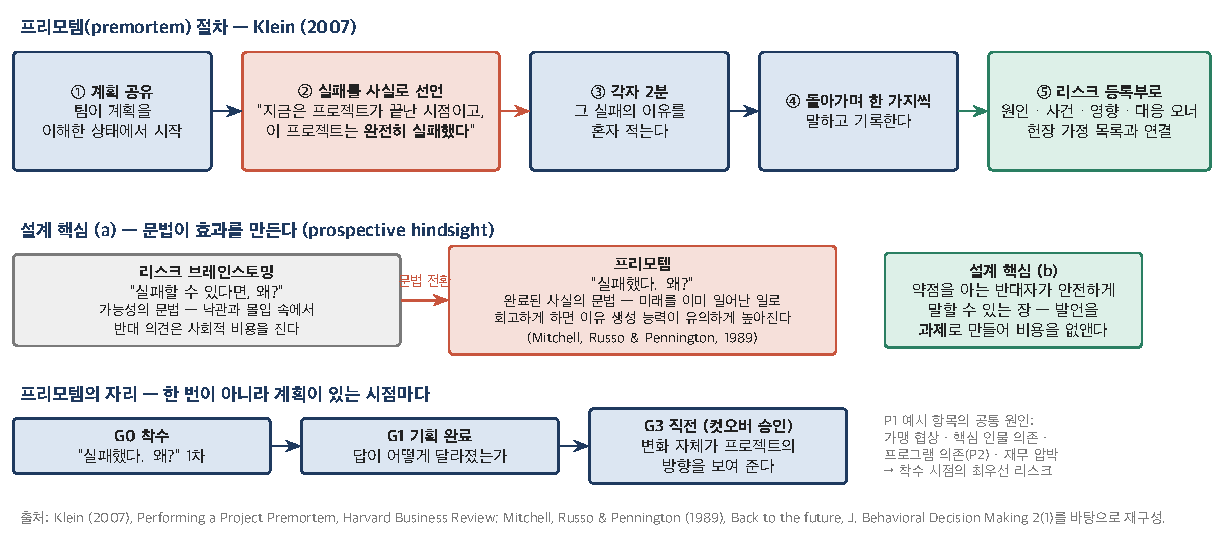
\includegraphics[width=1.00\textwidth,height=0.72\textheight,keepaspectratio]{../그림/PM_Day1/fig_3_5_premortem.pdf}
\par\nobreak\vspace{1pt}{\scriptsize\color{mDarkTeal!70}그림 3-7. 프리모템 절차와 "실패했다"의 문법\par}
\end{center}
\framebreak
\begin{itemize}
\item\relax 절차: 팀이 계획을 공유한 뒤 진행자가 말한다 — \textbf{"지금은 프로젝트가 끝난 시점이고, 이 프로젝트는 완전히 실패했다. 각자 2분 동안 그 실패의 이유를 적으라."} 그다음 돌아가며 한 가지씩 말하고 기록
\item\relax 설계 핵심 둘
\par\nobreak
\begin{itemize}
\item\relax (a) \textbf{"실패했다"를 완료된 사실로 전제} — "실패할 수 있다면 왜"가 아니라 "실패했다. 왜". Mitchell, Russo \& Pennington(1989) prospective hindsight 실험: 미래를 이미 일어난 일로 회고하게 하면 이유를 생성하는 능력이 유의하게 높아진다. \textbf{문법의 차이가 효과를 만든다}
\item\relax (b) \textbf{약점을 아는 반대자가 안전하게 말할 수 있는 장} — 킥오프 직후의 팀은 낙관과 몰입으로 차 있고 "이건 안 될 것 같다"의 사회적 비용이 크다. 프리모템은 그 발언을 \textbf{과제}로 만들어 비용을 없앤다
\end{itemize}
\item\relax P1에서 나올 법한 실패 이유 (교재 예시): 가맹 388점 중 140점이 새 POS 배포 거부, 두 시스템 병행 / G2 정본 결정이 박세연 한 사람에게 걸려 두 달 지연 / P2 41주로 물류 인터페이스 시험이 컷오버 후로 / CFO 148억 축소로 전환 용역 11.4억이 2027년으로, 리허설 3회$\rightarrow$1회 / 수행사 대기 시간 변경대가 청구, 변경협의체 6개월 미합의 / 오픈 첫 달 615개 매장 콜이 서비스데스크 11명에게, SAC 미충족으로 인수 거부
\item\relax 각 항목이 리스크 등록부 한 행(원인·사건·영향·오너)이 되고, \textbf{여러 항목이 같은 원인}(가맹 협상, 핵심 인물, 프로그램 의존, 재무 압박)을 가리키는 것이 보인다 $\rightarrow$ 그 공통 원인이 최우선 리스크
\end{itemize}
\begin{itemize}
\item\relax 실무 오류 다섯 (§3.5): 등록부를 "일반적 리스크 목록"(일정 지연·예산 초과·인력 이탈)으로 채움 / "실패했다"를 "실패할 수 있다"로 바꿔 브레인스토밍으로 / 결과를 헌장 가정·리스크 등록부에 연결 안 함 / 반대자의 발언을 분위기 해치는 것으로 / uniqueness bias("우리는 특별하다")를 리스크 식별에서 반복
\end{itemize}
\note{§3.5 "프리모템"과 "실무에서 어떻게 틀리는가". 세 번째 오류의 처방이 워크북 §5 항목 6(즉시 조치와 헌장·계획 반영). 게이트마다 반복한다 — G0, G1, G3 직전. "실패했다. 왜"의 답이 달라지는 것이 프로젝트가 어디로 가는지를 보여 준다. 6교시 워크북 §5에서 실패 선언문 세 개(일정·편익·중단)로 실습. 예상 소요 7분.}
\end{frame}

% ---- md slide 67: 분야별 착수 노하우 ① — SI: 계약 이후에 착수하는 프로젝트
\begin{frame}[allowframebreaks=1.0]{분야별 착수 노하우 ① — SI: 계약 이후에 착수하는 프로젝트}
\small
\begin{itemize}
\item\relax 결정적 차이: \textbf{착수 시점에 이미 계약이 있다.} RFP $\rightarrow$ 제안 $\rightarrow$ 평가 $\rightarrow$ 협상 $\rightarrow$ 계약이 끝나 있고 범위·금액·기간·산출물이 계약서에 있다. SI PM의 착수 시점 일은 헌장을 쓰는 것이 아니라 \textbf{계약 문서를 읽고 헌장으로 번역하는 것}
\item\relax 읽어야 할 것 셋
\par\nobreak
\begin{enumerate}
\item\relax \textbf{세 문서와 우선순위} — 통상 계약서 > 과업지시서(RFP) > 제안서. 제안서는 과업을 늘릴 수는 있어도 RFP를 축소할 수는 없는 \textbf{"단방향 확대 문서"} — 차별화로 쓴 "무상 3개월 안정화", "성능 2배", "AI 자동 분류"가 그대로 과업이 된다. 발주사 PM은 제안서에 쓰인 것을 착수 시점에 산출물 목록으로 확정해 둔다
\item\relax \textbf{규모 기준선} — FP 12,400점 $\times$ 55만 원 = 68.2억. FP는 객관적 측정치가 아니라 발주사에게는 상한, 수행사에게는 변경대가 근거로 작동하는 \textbf{협상 인공물}. 착수 시점 FP 기준선을 양측 서면 확인(G1 "FP 기준선 확인서 서명")해야 델타 주장이 성립. 응찰가 198억$\rightarrow$168억·손익률 6.5\% $\rightarrow$ 3주차에 WBS와 제안서 산출물이 1:1이 아니라고 밝혀지면 검수 분쟁 확정
\item\relax \textbf{인터페이스 상대의 소유자} — SI는 컷오버 주말에 죽지 않는다. 진짜 사인은 데이터 정제 착수 지연과 인터페이스 상대 미확정. 47본 중 문서 부재 13본, 3PL WMS, 별도 법인 공장 데이터, 은행·PG 7본 — \textbf{"누가 상대 쪽을 준비하는가"의 이름}이 없으면 통합시험에서 멈춘다
\end{enumerate}
\item\relax \textbf{공공 vs 민간} — 소프트웨어 진흥법 §50 과업심의위원회, 전자정부법 감리 의무, 분리발주는 \textbf{국가기관 등 공공 발주에만} 적용. 온담 같은 민간 발주에는 없다 $\rightarrow$ 그 기능은 계약서로 직접 만든다(사내 CCB + 변경협의체 + 기준선 재확인). 공공 경험자가 민간에서 "과업심의위원회에 올리자"고 말하는 순간 그 제도가 여기 없다는 사실이 리스크
\end{itemize}
\note{§3.6 "SI". 발주사 PM(수강생)과 수행사 PM(이재현)은 같은 프로젝트의 다른 이해관계를 갖는다는 1교시 §1.5의 이원 구조 재확인. 예상 소요 7분.}
\end{frame}

% ---- md slide 68: 분야별 착수 노하우 ② — 건설·EPC / 제조 NPD
\begin{frame}[allowframebreaks=1.0]{분야별 착수 노하우 ② — 건설·EPC / 제조 NPD}
\small
\par\smallskip\noindent{\usebeamercolor[fg]{normal text}\textbf{건설·EPC — 발주 방식과 계약 유형이 착수 전에 리스크를 결정한다}\par}\nobreak
\begin{itemize}
\item\relax \textbf{설계 성숙도}: AACE 추정 등급 Class 5(정의도 0\textasciitilde{}2\%) \textasciitilde{} Class 1(50\textasciitilde{}100\%). 어느 Class에서 계약하느냐가 신뢰 구간을 정한다 — 구간은 고정 상수가 아니라 리스크 분석으로 산정. "Class 3 = $-$20\%\textasciitilde{}+30\%"처럼 표를 외워 적용하면 틀린다
\item\relax \textbf{계약 유형}의 역설: Class 4 이하에서 경쟁입찰 LSTK를 맺으면 리스크가 이전되는 것이 아니라 (a) 프리미엄으로 얹히거나 (b) 시공자가 스펙을 동결하고 모든 해석 차이가 변경 청구가 되어 (c) 클레임·부실·부도로 되돌아온다(Merrow, IPA). \textbf{"턴키가 안전하다"는 신념이 깨지는 지점}
\item\relax 온담 P2가 정확히 이 검토 대상 — "4,200은 현장 숫자가 아니다" = Class 4 사양으로 설비 발주(선급금 29.6억)를 앞두고 있다
\item\relax \textbf{기록 규율}: SCL Protocol 2판 Core Principle 1 "프로그램과 기록" — 지연 청구의 승패는 분석 기법이 아니라 \textbf{사건 당시 생성된 기록}. SI에도 성립 — "발주사 결정 지연 12일"을 주장하려면 당일 서면 통지. 회의록 확인 서명을 미루기 시작하는 발주사 담당자는 내부적으로 결정 권한을 잃었다는 신호
\end{itemize}
\par\smallskip\noindent{\usebeamercolor[fg]{normal text}\textbf{제조 NPD — Stage-Gate의 Gate 1\textasciitilde{}2}\par}\nobreak
\begin{itemize}
\item\relax 정보가 가장 적은 시점의 결정. \textbf{게이트는 회의가 아니라 투자 결정} — Go / Kill / Hold / Recycle, Go에는 다음 스테이지 인력·예산이 붙어야. 자원 약정 없는 게이트 = "이빨 없는 게이트"
\item\relax \textbf{Must-meet / Should-meet 이원 기준} — 규제·안전·IP는 must-meet. "3.8점이니 통과"는 규제 불가 항목이 마케팅 점수에 가려진 것
\item\relax 초기 게이트에서 \textbf{전체 NPV를 요구하지 않는다} — 실물옵션: 각 스테이지 투자는 "다음 단계로 갈 권리를 사는 것"
\item\relax \textbf{Kill이 0건인 게이트 프로세스는 고장난 것} $\rightarrow$ 온담 G0\textasciitilde{}G5에 던질 질문: G1에서 P1을 중단할 수 있는가, 기준은, 중단 결정자는 착수 결정자와 다른 사람인가(마무리 §4.4 Staw)
\end{itemize}
\note{§3.6 "건설·EPC"와 "제조 NPD". EPC PM이 SI PM에게 줄 수 있는 것 — "추정치를 숫자 하나가 아니라 숫자 + 정확도 밴드 + 근거 산출물 목록으로 유통시키는 문화"(§1.5). 예상 소요 7분.}
\end{frame}

% ---- md slide 69: 분야별 착수 노하우 ③ — 제약·규제 / 네 분야가 착수에서 공유하는 것
\begin{frame}[allowframebreaks=1.0]{분야별 착수 노하우 ③ — 제약·규제 / 네 분야가 착수에서 공유하는 것}
\small
\par\smallskip\noindent{\usebeamercolor[fg]{normal text}\textbf{제약 — 규제 게이트의 비가역성}\par}\nobreak
\begin{itemize}
\item\relax 착수는 규제 경로 결정에서 시작: IND $\rightarrow$ 임상 $\rightarrow$ NDA / 510(k) · De Novo · PMA / SW 의료기기는 IEC 62304 등급(A/B/C). 경로가 정해지면 게이트는 협상 불가
\item\relax 세 특징: (a) \textbf{제출 순간 문서 세트가 잠긴다} (b) \textbf{심사 시계는 제출자가 통제 못 한다} — De Novo 150일은 응답 대기 제외 심사일 (c) \textbf{추가자료 요구는 시계를 멈추고 재개 시점을 상대가 정한다} $\rightarrow$ float 개념이 성립하지 않는다
\item\relax 착수 오류: 규제 마일스톤을 표준 심사 기간 고정 블록으로 놓고 \textbf{추가자료 라운드 0회로 가정}한 뒤 출시일을 공표. 처방: 라운드 수를 같은 경로의 과거 제출 건(reference class)에서 분포로
\item\relax "규제가 애자일을 막는다"는 통념은 틀렸다 — GAMP 5 2판, FDA CSA. 개발 리듬(스프린트)과 산출물 베이스라인(릴리즈)을 분리
\item\relax 온담 P4: 개인정보 보호법 개정 대응(2026-09-11, 처리항목 142개·위탁사 19개), 전자금융업 등록(신청 2027-01-29, 심사 2027-03-31), ISMS-P(2027-06). 최영주: "시행일은 협상 대상이 아니다" / "검토 의견을 제공하지 아키텍처를 결정하지 않는다" — \textbf{규제 해석을 착수 시점에 서면으로 받아 두라}
\end{itemize}
\par\smallskip\noindent{\usebeamercolor[fg]{normal text}\textbf{네 분야가 착수에서 공유하는 네 질문}\par}\nobreak
\begin{itemize}
\item\relax \textbf{무엇이 이미 결정되어 있는가} (계약, 설계 성숙도, 규제 경로, 게이트 기준)
\item\relax \textbf{어느 결정이 되돌릴 수 없는가} (FP 기준선, 설비 발주, 금형, 규제 제출)
\item\relax \textbf{누가 그 결정을 소유하는가}
\item\relax \textbf{그것을 문서로 남겼는가} — 헌장은 이 네 질문의 답을 적는 곳
\end{itemize}
\note{§3.6 "제약"과 "네 분야가 착수에서 공유하는 것". 온담은 제약회사가 아니지만 P4 규제 워크스트림이 같은 구조라는 점으로 연결. 예상 소요 6분.}
\end{frame}

% ---- md slide 70: 5교시 핵심 정리
\begin{frame}[allowframebreaks=1.0]{5교시 핵심 정리}
\small
\begin{enumerate}
\item\relax 거버넌스는 조직도가 아니라 \textbf{결정의 흐름}. 허용범위 격자(7축 $\times$ 3계층)가 PM이 권한을 얻는 유일한 표준 근거 경로 — 사내 전결 규정과 BC 편익 민감도 양쪽으로 검증
\item\relax 권한 없는 PM은 구조의 문제(매트릭스 / 직위 기준 전결 / 위임 없는 보고 요구). 처방 셋 — \textbf{허용범위를 서명으로 획득 / 결정을 선택지·권고·기한과 함께 가져간다 / 에스컬레이션을 BATNA로 쓰지 않는다}
\item\relax 착수 시점 리스크는 \textbf{가정·구조·base rate}에서 나온다. 자기 과거 실적을 알아도 예측은 개선되지 않는다(Buehler et al.) $\rightarrow$ outside view
\item\relax 프리모템(Klein, 2007)은 \textbf{"실패했다. 왜"}의 문법으로 반대자의 발언을 과제로 만든다. 게이트마다 반복하고, 결과를 헌장 가정과 리스크 등록부에 연결한다
\item\relax SI는 \textbf{계약 이후 착수}(문서 우선순위, FP 기준선, 인터페이스 소유자 — 공공 제도는 민간에 없다) / EPC는 \textbf{설계 성숙도 $\times$ 계약 유형} / NPD는 \textbf{자원 약정이 붙은 Gate 1\textasciitilde{}2, kill 0건이면 고장} / 제약은 \textbf{규제 게이트의 비가역성}
\end{enumerate}
\note{제3장 핵심 정리 6\textasciitilde{}8. 6교시는 바로 실습 ②(워크북 §3 등록부, §4 거버넌스·RACI, §5 프리모템). 4교시에 쓴 헌장 초안을 꺼내 놓게 한다 — §3\textasciitilde{}5는 헌장을 고치는 문서들이다. 예상 소요 3분.}
\end{frame}

\section{6교시 (75분) — 실습 ②: 이해관계자 등록부 · 거버넌스·RACI · 프리모템}

% ---- md slide 71: 이 교시에서 하는 것
\begin{frame}[allowframebreaks=1.0]{이 교시에서 하는 것}
\small
\begin{itemize}
\item\relax \textbf{산출물 ③ 이해관계자 등록부와 현저성 분석} — 워크북 §3. 약 25분
\item\relax \textbf{산출물 ④ 거버넌스 구조와 RACI 초안} — 워크북 §4. 약 20분
\item\relax \textbf{산출물 ⑤ 프리모템 기록과 초기 리스크 목록} — 워크북 §5. 약 25분
\item\relax 세 문서는 4교시에 쓴 헌장을 \textbf{고치는} 문서다 — 등록부가 헌장 항목 11을, RACI가 항목 12를, 프리모템이 항목 9·10을 되먹인다 (워크북 §6)
\item\relax 진행 방식: 과제 지시 $\rightarrow$ 작성 요령 $\rightarrow$ 흔한 오류 $\rightarrow$ 예시본 대조. 프리모템은 조별로 실제로 실시한다
\item\relax 준비물: 워크북 §3.4·§4.4·§5.4 빈 템플릿, §3.5·§4.5·§5.5 완성 예시본, 4교시 헌장 초안
\end{itemize}
\note{75분에 세 산출물이므로 각 산출물은 핵심 항목만 채운다 — 등록부는 인물 6\textasciitilde{}8명의 3속성·유형·관계 소유자, RACI는 10행, 프리모템은 실패 선언문 1개 + 사유 수집 + 리스크 3행. 나머지는 예시본 대조와 사후 과제. 예상 소요 3분.}
\end{frame}

% ---- md slide 72: 산출물 ③ 이해관계자 등록부 — 과제 지시
\begin{frame}[allowframebreaks=1.0]{산출물 ③ 이해관계자 등록부 — 과제 지시}
\small
\begin{itemize}
\item\relax \textbf{과제}: 워크북 §3.4 템플릿으로 다음 8명을 등록하라 — \textbf{정미란·오정근·박세연·한동석·서정필·김미르·최영주·박준영}. 각 행에 항목 3(기대·우려·KPI), 항목 4(P/L/U 3속성과 7유형), 항목 5(태도 현재$\rightarrow$목표), 항목 6(관여 전략·\textbf{관계 소유자})을 채우라. 그다음 \textbf{현저성 분석 요약표}(유형별 인물·대응 원칙)를 만들라
\item\relax 등록부의 가치는 명단이 아니라 \textbf{분석 열}에 있다 — 어떤 힘이 있는가, 쓸 정당성이 있는가, 지금 움직이려 하는가. 그리고 그 셋은 \textbf{바뀐다}
\item\relax 이 문서가 없을 때 터지는 것 (워크북 §3.1): \textbf{보이지 않던 사람이 결정적 순간에 나타난다}(김미르 — P1은 인력 프로젝트가 아니지만 이천센터 협조 없이 데이터 전환도 시험도 안 된다) / \textbf{같은 직책을 같은 방식으로 대한다}(오정근과 한동석은 둘 다 본부장이지만 P1에 대한 긴급성·정당성 구조가 다르다 — 같은 월간 보고서를 보내면 둘 다에게 외면당한다)
\item\relax 분야별 무게 중심: SI는 현업-IT 긴장과 계약 관계, \textbf{최종 사용자가 가장 자주 누락} / EPC는 인허가·주민·환경단체·하도급이 절반 / NPD는 핵심 고객·인증기관·단일소스 부품사, \textbf{양산 이관받는 생산·품질이 누락}. 규칙은 같다 — \textbf{"요구할 정당성은 없지만 멈출 힘이 있는 사람"}을 찾아 적는 것이 등록부의 절반
\end{itemize}
\note{워크북 §3.1\textasciitilde{}3.2. 표준 위치: PMBOK 8판 Stakeholders 도메인(Communications 흡수) / 6판 13.1·13.2(태도 5단계 표기법의 유래) / PRINCE2 organizing + communication management approach / ISO 21502 §7.12. 예상 소요 4분.}
\end{frame}

% ---- md slide 73: 작성 요령 ⑤ — 3속성 판정 · 태도 · 관계 소유자 (워크북 §3.3 항목 3~6)
\begin{frame}[allowframebreaks=1.0]{작성 요령 ⑤ — 3속성 판정 · 태도 · 관계 소유자 (워크북 §3.3 항목 3\textasciitilde{}6)}
\small
\par\smallskip\noindent{\usebeamercolor[fg]{normal text}\textbf{항목 3 관심사·기대·우려} — \textbf{그 사람의 말로} 적는다(정본의 "입장 한 줄"). 기대와 우려를 분리. 가능하면 KPI(오정근: 가맹 재계약률 91\%)\par}\nobreak
\begin{itemize}
\item\relax 박세연 — 기대: IT본부가 운영 가능한 아키텍처 / 우려: 벤더 종속, 그리고 \textbf{자신이 만든 OD-POS와 문서 없는 13본이 "실패"로 서술되는 것} — 공식 입장에 없지만 등록부에는 있어야 한다
\end{itemize}
\par\smallskip\noindent{\usebeamercolor[fg]{normal text}\textbf{항목 4 현저성 3속성과 유형} — P(이 프로젝트의 결정·자원·진행을 바꿀 수 있는가) / L(조직·계약·법적으로 정당한가) / U(지금 당장 대응을 요구하는가). \textbf{판정 시점(G0)}을 적고, 바뀔 시점과 방향을 비고에\par}\nobreak
\begin{itemize}
\item\relax 정미란 P+L+U 확정 / 김선호 P+L 지배 $\rightarrow$ G3에서 확정 / 서정필 L+U 의존 $\rightarrow$ 부속서 협상(2026-08)에서 388점 거부권이 실질 권력이 되어 확정 / \textbf{김미르 P(현장 협조 거부)+U 위험} / 윤태호 L+U 의존 $\rightarrow$ 감사 착수 시 P 획득
\item\relax 오류: 직급으로 권력 판정(본부장이면 모두 상 — 나영선의 P1 권력은 CCB 표 하나) / 긴급성 무시 / 한 번 판정하고 갱신 안 함
\end{itemize}
\par\smallskip\noindent{\usebeamercolor[fg]{normal text}\textbf{항목 5 태도} — 무인지/저항/중립/지지/주도. "현재 $\rightarrow$ 목표". 모두를 주도로 만들 필요 없다. \textbf{저항은 정보다}(Ford, Ford \& D'Amelio, 2008) — 오정근의 저항은 2019년의 경험이고 그것이 리스크 목록을 채운다\par}\nobreak
\begin{itemize}
\item\relax 오정근 저항(조건부)$\rightarrow$지지 / 박세연 중립(경계)$\rightarrow$주도 / 강윤지 저항(불신)$\rightarrow$지지(슈퍼유저) / 이재현 중립(계약 방어)$\rightarrow$지지
\end{itemize}
\par\smallskip\noindent{\usebeamercolor[fg]{normal text}\textbf{항목 6 관여 전략·채널·빈도·관계 소유자} — 정보 제공/협의/공동 결정/협상/모니터링 + \textbf{관계 소유자 실명}. 외부 협상 상대의 소유자는 PM이 아니라 소관 임원\par}\nobreak
\begin{itemize}
\item\relax 서정필 — 협상(소유자 \textbf{오정근}), P1은 가맹 포털 프로토타입 시연으로 지원 / 김미르 — 모니터링·정보 제공(소유자 \textbf{한동석}), "P1은 인력 프로젝트가 아님"을 문서로 / 윤태호 — 정보 제공(소유자 P1 PM), 컨틴전시 집행 기록 월 1회 사본
\end{itemize}
\note{워크북 §3.3. 항목 1(ID S-01 형식, 내부/외부·계약/비계약 구분), 항목 2(역할은 헌장 항목 12·RACI와 일치), 항목 7(갱신 시점 — G1, 2026-08 협상 후, G2, G3)은 구두로. 예상 소요 8분.}
\end{frame}

% ---- md slide 74: 산출물 ③ 흔한 오류 점검 + 예시본 참조
\begin{frame}[allowframebreaks=1.0]{산출물 ③ 흔한 오류 점검 + 예시본 참조}
\small
\par\smallskip\noindent{\usebeamercolor[fg]{normal text}\textbf{흔한 오류} (워크북 §3.3 각 항목)\par}\nobreak
\begin{itemize}
\item[$\square$]\relax 부서명만 적고 사람을 안 적었다 ("영업본부") — 부서는 우려를 갖지 않는다 / 임원만 적고 실무 접점자(구매팀장, 재경팀장, 지역매니저)를 뺐다
\item[$\square$]\relax "영향받는 자"(매장 직원, 물류 현장)를 유형에서 뺐다 — 요구하지 않지만 결과를 매일 겪는다
\item[$\square$]\relax PM의 추측을 그 사람의 기대로 / 우려를 안 적음 / 모두에게 "프로젝트 성공"
\item[$\square$]\relax 모두 "지지" / 목표를 모두 "주도" / 저항을 개인의 결함으로
\item[$\square$]\relax 전략 칸에 "정기 보고"만 / 관계 소유자를 안 적어 PM이 노조 협상까지 / 채널을 전부 회의로
\item[$\square$]\relax 착수 시 한 번 쓰고 끝 / 판정 시점이 없어 어느 시점의 판단인지 모름
\end{itemize}
\par\smallskip\noindent{\usebeamercolor[fg]{normal text}\textbf{예시본과 대조할 것} (워크북 §3.5\textasciitilde{}3.6, 25행 + 요약표 + 속성 변화 예측)\par}\nobreak
\begin{itemize}
\item\relax 왜 김미르를 "위험"으로 판정했는가 — 정당한 경로가 없는 권력은 비공식 경로로 행사된다. 대응은 설득이 아니라 \textbf{정당성 경로를 만들어 주는 것}(인사본부 협의 채널, P1 편익에 인건비 없음을 문서로). 2$\times$2로는 이 판단을 할 수 없다
\item\relax 왜 박세연의 "우려" 칸에 공식 입장에 없는 것을 / 왜 관계 소유자가 PM이 아닌 행이 열 개 가까이 / 왜 사모펀드와 규제기관처럼 접촉하지 않는 이해관계자를 넣었는가(등록부는 접촉 명단이 아니라 \textbf{힘의 지도}) / 왜 정하늘 감리원의 목표 태도가 중립$\rightarrow$중립인가(감리는 독립성이 가치)
\end{itemize}
\par\smallskip\noindent{\usebeamercolor[fg]{normal text}\textbf{점검 질문} (§3.7): 부서명만 있는 행이 있는가 / 관계 소유자가 전부 PM인가 / "우려" 칸이 "기대" 칸과 다른 내용인가\par}\nobreak
\note{12분 작성 후 5분 대조. §3.7 기본 과제(2026-06 3PL 협상 결렬 + P2 41주 확정 시 한동석·김미르·대성로지스·박준영 네 행 재판정, 헌장 항목 9의 어느 가정이 깨지는가)는 사후 과제. 예상 소요 4분.}
\end{frame}

% ---- md slide 75: 산출물 ④ 거버넌스 구조와 RACI — 과제 지시 + 작성 요령
\begin{frame}[allowframebreaks=1.0]{산출물 ④ 거버넌스 구조와 RACI — 과제 지시 + 작성 요령}
\small
\begin{itemize}
\item\relax \textbf{과제}: 워크북 §4.4 템플릿의 \textbf{항목 2(3역할과 핵심 직위)}와 \textbf{항목 5(RACI)} 10행을 채우라. 항목 1(의사결정체 목록)·3(에스컬레이션)·4(허용범위 3층)는 §4.5 예시본을 읽고 확인
\item\relax 거버넌스 구조 = "누가 무엇을 결정하는가", RACI = 각 결정·산출물에 대해 \textbf{R}(실행) / \textbf{A}(최종 책임, 행마다 정확히 한 명) / \textbf{C}(협의) / \textbf{I}(통보). 헌장 항목 12의 요약을 결정 단위로 펼친 것
\item\relax \textbf{RACI 규칙 셋} (워크북 §4.1): 행마다 A는 정확히 한 명 / R은 여럿일 수 있으나 조정자 필요 / C가 많으면 느려지고 I가 많으면 아무도 안 읽는 보고서. 그리고 \textbf{행은 활동이 아니라 결정과 산출물} — "회의 참석"은 행이 아니다
\item\relax \textbf{항목 2 3역할} — Executive 정미란 / Senior User 오정근(P3 겸임, 이해 충돌 없음) / Senior Supplier \textbf{박세연}(수행사 이재현은 그 아래의 공급자). 한 사람이 두 역할이면 명시하고 이해 충돌 여부를 적는다
\par\nobreak
\begin{itemize}
\item\relax 오류: 스폰서가 둘이거나 없다 / Senior User를 IT 부서장이 겸함(현업이 요구사항에 책임 안 짐) / \textbf{수행사 PM을 Senior Supplier로 적어 발주사 IT의 기술 승인 권한이 사라짐} — 한국 SI에서 가장 흔한 혼동
\end{itemize}
\item\relax \textbf{항목 5 RACI} — 행 = 결정과 산출물 15\textasciitilde{}25행, 열 = 역할·개인 8\textasciitilde{}12열. 결정 행과 산출물 행 구분. \textbf{통제 밖 결정(3PL 협상, 가맹 배포 범위, P2 규격)의 A가 P1 밖의 임원임을 명시}. 표 아래에 "A 없는 행 / A 둘인 행 = 0" 검산 문장
\par\nobreak
\begin{itemize}
\item\relax "컨틴전시 집행" 행: \textbf{A = P1 PM, C = 재경팀장, I = 정미란·윤태호} — 2020 감사 지적("승인 근거 없음")에 대한 답은 사전 승인이 아니라 \textbf{사후 투명성}
\end{itemize}
\end{itemize}
\note{워크북 §4.1\textasciitilde{}4.3. 이 문서가 없을 때 온담에서 터지는 것 셋 — 컨틴전시 승인 근거 부재(2020 감사) / 결정의 이중화(CCB vs 변경협의체가 같은 변경을 다른 각도에서) / 경계 결정의 공백(3PL·가맹·P2 규격은 PM이 R이지 A가 아닌데 A가 적혀 있지 않으면 아무도 안 한다). 항목 1의 관계 문장 "변경협의체 합의 $\rightarrow$ CCB 승인 $\rightarrow$ 계약 변경"과 항목 3의 시한(수행사 PM $\rightarrow$ P1 PM 3영업일 $\rightarrow$ 스폰서 5영업일 $\rightarrow$ 이사회 임시 소집 10영업일, 발주사 응답 시한 5영업일 초과 시 대기 비용 산정 개시)은 구두로. 예상 소요 8분.}
\end{frame}

% ---- md slide 76: 산출물 ④ 흔한 오류 점검 + 예시본 참조
\begin{frame}[allowframebreaks=1.0]{산출물 ④ 흔한 오류 점검 + 예시본 참조}
\small
\par\smallskip\noindent{\usebeamercolor[fg]{normal text}\textbf{흔한 오류} (워크북 §4.3)\par}\nobreak
\begin{itemize}
\item[$\square$]\relax 회의체 이름만 적고 권한을 안 적음 / 정족수·반대의견 기록 방식이 없어 "전원 찬성"만 남음 / 사내 CCB와 계약상 변경협의체의 선후 관계를 안 적음
\item[$\square$]\relax 경로는 있는데 시한이 없다 / "필요 시 보고"(필요는 항상 사후에 판정된다) / 수행사의 에스컬레이션 경로를 뺐다
\item[$\square$]\relax 모든 프로젝트에 같은 $\pm$10\% — 허용범위는 BC 편익 민감도(손익분기 66\%)에서 역산 / 작업패키지 계층을 비워 수행사에 아무 재량도 안 줌
\item[$\square$]\relax \textbf{A가 둘 이상인 행(공동 책임 = 무책임)} / PM이 모든 행의 A / 활동("주간 회의")을 행으로 / 위원회와 개인이 섞인 열에서 위원회 안의 누가 A인지 불명확
\end{itemize}
\par\smallskip\noindent{\usebeamercolor[fg]{normal text}\textbf{예시본과 대조할 것} (워크북 §4.5\textasciitilde{}4.6, 26행 RACI)\par}\nobreak
\begin{itemize}
\item\relax \textbf{왜 P1 PM이 A인 행이 26개 중 8개뿐인가} — 착수·기획 결정 26개 중 18개의 최종 책임은 PM 밖에 있다(3PL 한동석, 가맹 배포 오정근, 아키텍처 박세연, 규제 해석 최영주, 기준선 이사회). 이 표를 스폰서에게 보여 주는 이유는 PM 책임을 줄이려는 것이 아니라 \textbf{A인 사람들이 자기가 A라는 것을 알게 하기 위해서}. 2022 WMS 회의록의 비어 있는 서명란은 그가 A였다는 것을 아무도 문서로 말하지 않았기 때문
\item\relax 왜 컨틴전시 집행의 A를 PM으로 두고 CCB를 I로 / 왜 가맹 SW 배포 범위(A 오정근)에 CCB·정미란을 C로(C를 빼면 배포 범위가 조용히 줄고 P1은 G2에서 발견) / 왜 CCB와 변경협의체 순서를 문장으로 못박았는가 / 왜 박세연의 이해 충돌(교체 대상 시스템의 설계자가 아키텍처 승인자)을 표에 기록했는가 — 데이터 전환 정본 판정에서 그는 R이지 A가 아니고 감리 확인 병행
\end{itemize}
\par\smallskip\noindent{\usebeamercolor[fg]{normal text}\textbf{점검 질문} (§4.7): 모든 행에 A가 정확히 한 명인가 / PM이 A가 아닌 행의 A들이 자기가 A라는 사실을 서명으로 확인했는가 — \textbf{확인하지 않은 A는 A가 아니다} / 사내 회의체와 계약상 회의체가 같은 변경을 어떤 순서로 다루는지 한 문장으로\par}\nobreak
\note{10분 작성 후 5분 대조. 심화 과제(§4.7): 자기 회사 운영위 명단에 3역할 배정 $\rightarrow$ 배정 안 되는 인물 수와 빈 역할, 최근 결정 10개로 RACI $\rightarrow$ A가 둘이거나 없는 행 수. 예상 소요 4분.}
\end{frame}

% ---- md slide 77: 산출물 ⑤ 프리모템 — 과제 지시 (조별로 실제로 실시한다)
\begin{frame}[allowframebreaks=1.0]{산출물 ⑤ 프리모템 — 과제 지시 (조별로 실제로 실시한다)}
\small
\begin{itemize}
\item\relax \textbf{과제}: 조별로 프리모템을 실시하고 워크북 §5.4 템플릿의 항목 2(실패 선언문) · 3(원문) · 4(군집화) · 5(초기 리스크 목록 3행) · 6(즉시 조치)을 채우라
\item\relax \textbf{절차} (워크북 §5.3, Klein 2007)
\par\nobreak
\begin{enumerate}
\item\relax 진행자가 \textbf{실패 선언문}을 읽는다 — 과거형, 날짜·숫자 포함. 예: F1 "2027-08, 컷오버 창을 놓쳐 IPO 예비심사 서류에 '구축 중'으로 기재되었다" / F2 "2028-03-31 G5에서 편익 실현률 41\%로 판정되었다" / F3 "2026-11 G2에서 프로그램 이사회가 P1 중단을 의결했다"
\item\relax 각자 \textbf{2분간 개별 작성} — "무엇이 일어났다"의 과거형. "\textasciitilde{}할 것 같다"는 다시 쓰게 한다
\item\relax 돌아가며 한 가지씩 말하고 \textbf{편집 없이} 번호를 붙여 기록. 중복도 그대로(중복 횟수가 우선순위 정보)
\item\relax 유사 원인별로 군집화, 언급 수 + 1인 3표로 순위. 군집명은 범주("일정")가 아니라 \textbf{원인}("가맹 부속서 협상 지연")
\end{enumerate}
\item\relax 왜 착수 리스크 식별의 첫 도구인가 (워크북 §5.1): 착수 시점 편향(낙관, 계획 오류, 고유성)이 가장 강하고 그 절반은 정치적 편향. 브레인스토밍은 "요구사항 변경" 같은 안전한 일반론을, 프리모템은 "협의회가 단말 비용 문제로 2026-08 부속서 서명을 거부했고 그때 우리는 이미 가맹 SW를 개발 중이었다"를 낸다
\item\relax 분야별: SI는 발주사 내부·계약 경계가 대부분, 기술 리스크는 의외로 적음. 수행사 포함 여부는 논쟁적 — \textbf{발주사 세션과 합동 세션 분리}가 절충 / EPC는 HAZOP·Constructability Review가 제도화 / NPD는 FMEA가 부품·공정 단위 프리모템
\end{itemize}
\note{워크북 §5.1\textasciitilde{}5.3. 조당 5\textasciitilde{}6명, 진행자는 강사가 아니라 조원 중 한 명. 세션 정보(항목 1)는 참가자를 역할로 적어도 된다 — 익명성이 기법의 전제. 실패 선언문 세 개를 다 쓰면 좋지만 시간상 F1 또는 F2 하나로. 예상 소요 5분 (설명) + 실시 12분.}
\end{frame}

% ---- md slide 78: 작성 요령 ⑥ — 리스크 서술 3부 · 소유자 · 즉시 조치 (워크북 §5.3 항목 5~6)
\begin{frame}[allowframebreaks=1.0]{작성 요령 ⑥ — 리스크 서술 3부 · 소유자 · 즉시 조치 (워크북 §5.3 항목 5\textasciitilde{}6)}
\small
\par\smallskip\noindent{\usebeamercolor[fg]{normal text}\textbf{항목 5 초기 리스크 목록} — 군집을 리스크 서술로 전환. 각 행: ID / \textbf{원인 $\rightarrow$ 사건 $\rightarrow$ 영향} / 범주 / 출처(군집 번호, 헌장 가정 번호) / 정성 확률·영향(상중하) / 근접성 / \textbf{소유자(실명)} / 초기 대응 방향 / 트리거 신호 / 다음 검토. \textbf{기회 1\textasciitilde{}2건 포함}\par}\nobreak
\begin{itemize}
\item\relax 서술 3부의 규율: 원인은 \textbf{현재 사실}, 사건은 \textbf{불확실한 미래}, 영향은 \textbf{목표에의 결과}
\par\nobreak
\begin{itemize}
\item\relax 예시본 R-01: "P2 설비 벤더가 리드타임 34$\rightarrow$41주 가능성을 통지한 상태다 $\rightarrow$ MC가 2027-02-12를 넘겨 2027-04 이후가 된다 $\rightarrow$ 물류 인터페이스 통합시험을 G3 전에 못 하고 컷오버를 분리하거나 창을 놓친다"
\item\relax 원인을 적으면 \textbf{트리거}(T0에서 확정)를, 사건을 적으면 \textbf{근접성}을, 영향을 적으면 \textbf{대응 방향}(분리 가능한 설계)을 알 수 있다. Day2 정량화는 확률을 사건에, 금액을 영향에 붙인다
\end{itemize}
\item\relax 소유자는 리스크의 원인에 가장 가까이 있고 대응 자원을 가진 사람 — \textbf{PM이 아닌 경우가 많다}. 예시본 13개 위협 중 PM 소유는 3개(R-07 요구사항 집중, R-13 컷오버 단말, R-04 대응안)
\item\relax 오류: 원인과 사건을 섞음("P2 지연 리스크" — 지연은 사건, 원인은 41주 통지) / 영향 없음 / 소유자 전부 PM / \textbf{이미 발생한 이슈}(OD-POS OS 종료는 사실이지 리스크가 아님)를 리스크로 / 기회를 안 적음
\end{itemize}
\par\smallskip\noindent{\usebeamercolor[fg]{normal text}\textbf{항목 6 즉시 조치와 헌장·계획 반영} — 리스크 대응 계획을 기다리지 않고 \textbf{지금 바꿔야 하는 것}: 헌장 가정·제약·제외 범위 수정, 등록부 추가, RACI 행 추가. 각 줄에 "어느 문서의 어느 항목을 어떻게" + 담당·기한\par}\nobreak
\begin{itemize}
\item\relax 예시본: 헌장 가정에 "자사앱 벤더 연동 2026-12" 추가(원문 8번이 드러냄) / 등록부 S-19 자사앱 벤더를 \textbf{위험} 유형으로 / RACI 12행(앱 소스 인수) 추가 / BC 가정 A3(분모)에 R-12 연결, 편익 책임자 서명을 G1 통과 조건에 / 가맹 단말 기종 전수 조사(R-13) 착수 요청 — 오정근, 2026-04
\end{itemize}
\note{워크북 §5.3 항목 5·6과 §5.6 해설. 오류 3번(결과가 리스크 목록에만 남고 헌장은 그대로)의 처방이 항목 6이다 — "다섯 문서는 서로를 고친다". 예시본의 기회 O-02(가맹 포털을 2026-Q4 먼저 릴리스하면 부속서 협상의 지렛대 $\rightarrow$ R-02 확률 감소)가 프리모템에서 나온 가장 실용적 발견. 예상 소요 7분.}
\end{frame}

% ---- md slide 79: 산출물 ⑤ 흔한 오류 점검 + 예시본 참조
\begin{frame}[allowframebreaks=1.0]{산출물 ⑤ 흔한 오류 점검 + 예시본 참조}
\small
\par\smallskip\noindent{\usebeamercolor[fg]{normal text}\textbf{흔한 오류} (워크북 §5.3, 교재 §3.5)\par}\nobreak
\begin{itemize}
\item[$\square$]\relax 실패 선언문을 조건문으로("만약 \textasciitilde{}한다면") — 그러면 프리모템이 아니라 브레인스토밍 / 실패의 모습이 추상적("잘 안 됐다") / 한 종류의 실패만 제시해 사유가 한쪽으로 쏠림
\item[$\square$]\relax PM 혼자 쓴다(PM의 걱정 목록) / 임원이 참석해 발언 위축 / 운영·현업이 없어 기술 리스크만
\item[$\square$]\relax 수집 단계에서 토론이 시작되어 사유가 걸러진다 / PM이 "그건 이미 대응 중"이라며 삭제 / 원문을 곧바로 범주("일정", "인력")로 뭉갬
\item[$\square$]\relax 군집을 너무 크게("외부 요인") / 득표만 보고 언급 수 적은 치명적 사유(원 개발자 1명 이탈)를 탈락시킴
\item[$\square$]\relax 리스크 목록이 일반론 / 소유자 전부 PM / 이미 발생한 이슈를 리스크로 / 결과를 헌장에 연결 안 함
\end{itemize}
\par\smallskip\noindent{\usebeamercolor[fg]{normal text}\textbf{예시본과 대조할 것} (워크북 §5.5\textasciitilde{}5.6 — 세션 정보, 실패 선언문 F1\textasciitilde{}F3, 원문 15개, 군집 12개, 리스크 R-01\textasciitilde{}R-13 + O-01·O-02, 즉시 조치 7건)\par}\nobreak
\begin{itemize}
\item\relax 왜 실패 선언문을 세 개로 — F1만 주면 사유가 전부 일정으로 쏠린다. F2(제때 끝나도 편익 실패), F3(통제 밖의 것이 결합해 중단). Flyvbjerg의 iron law(세 성공은 별개)를 프리모템 설계로 옮긴 것
\item\relax 왜 리스크 서술을 세 부분으로 강제했는가 / 왜 소유자에 PM이 세 번밖에 없는가(RACI 8/26과 같은 그림) / 왜 기회를 넣었는가 / 왜 "즉시 조치"에서 헌장을 고쳤는가
\end{itemize}
\par\smallskip\noindent{\usebeamercolor[fg]{normal text}\textbf{점검 질문} (§5.7): 실패 선언문이 과거형인가 / 리스크 "원인"이 지금 확인 가능한 사실인가 / \textbf{소유자 열에서 PM이 절반을 넘는가} — 넘는다면 통제 밖 리스크를 PM이 떠안고 있거나 아직 못 찾은 것\par}\nobreak
\note{조별 리스크 3행을 발표시키고 "원인이 현재 사실인가"만 검사한다. §5.7 기본 과제(2026-02-16 내부통제 지침 — 5,000만 원 이상 CFO 직접 결재를 컨틴전시에도 적용 $\rightarrow$ R-14 서술, R-04·R-05와의 결합)는 사후 과제. 예상 소요 4분.}
\end{frame}

% ---- md slide 80: 다섯 문서의 상호 관계 — 순서대로 쓰지만 순서대로 완성되지 않는다
\begin{frame}[allowframebreaks=1.0]{다섯 문서의 상호 관계 — 순서대로 쓰지만 순서대로 완성되지 않는다}
\small
{\usebeamercolor[fg]{normal text}
\begin{center}
\begin{tikzpicture}[
  doc/.style={draw=mDarkTeal, rounded corners=2pt, fill=mDarkTeal!6, align=center,
              font=\scriptsize\bfseries, inner sep=4pt, minimum height=8mm, text width=36mm},
  lab/.style={font=\tiny, text=black!75, align=center, inner sep=1pt},
  arr/.style={-{Stealth[length=2mm]}, thick, draw=mDarkTeal}, x=1mm, y=1mm]
\node[doc] (bc)   at (0,0)    {비즈니스 케이스 요약};
\node[doc] (ch)   at (95,0)   {헌장 §2 목적 / §3 성공 기준\\/ §14 중단 조건};
\node[doc] (pm)   at (0,-24)  {프리모템·초기 리스크};
\node[doc] (sr)   at (95,-24) {이해관계자 등록부};
\node[doc] (ch2)  at (0,-48)  {헌장 §9·§10 수정 (v1.1)};
\node[doc] (raci) at (95,-48) {거버넌스·RACI};
\draw[arr] (bc) -- node[lab, above] {편익 118억·손익분기 66\%·승인 조건 5} (ch);
\draw[arr] (ch) -- node[lab, left, text width=34mm] {범위 경계·제외 범위·가정·제약} (sr);
\draw[arr] (sr) -- node[lab, above] {누가 경계 안팎에 있는가 / 가정 1$\sim$6 $\rightarrow$ 리스크 원인} (pm);
\draw[arr] (pm) -- node[lab, right, text width=30mm] {분모 가정 A3 $\leftarrow$ R-12} (bc);
\draw[arr] (pm) -- node[lab, right, text width=30mm] {소유자 실명, 즉시 조치} (ch2);
\draw[arr] (sr) -- node[lab, left, text width=34mm] {현저성 유형 $\rightarrow$ 의사결정체 배정, 관계 소유자} (raci);
\draw[arr] (raci) -- node[lab, below] {A가 누구인가 $\rightarrow$ 리스크 소유자, 에스컬레이션 경로} (ch2);
\end{tikzpicture}
\end{center}
}
\begin{itemize}
\item\relax BC $\rightarrow$ 헌장: 목적은 118억·규제 기한을 인용, 성공 기준의 편익 층은 편익 표를 그대로, 중단 조건 66\%는 재무 평가에서
\item\relax 헌장 $\rightarrow$ 등록부: 가맹 단말 HW를 제외 범위에 넣는 순간 서정필의 우려가 등록부의 한 칸이 되고, 3PL 경계 조건을 적는 순간 대성로지스가 휴면 유형으로
\item\relax 등록부 $\rightarrow$ RACI: 확정 유형 4명 = 3역할 + 수행사 PM = 기준선 동결의 필수 합의자. 위험 유형의 관계 소유자(한동석·박세연) = RACI 해당 행의 A
\item\relax 헌장·등록부·RACI $\rightarrow$ 프리모템: 가정 6개가 R-01·02·03·05·08의 원인. RACI의 A가 리스크 소유자
\item\relax 프리모템 $\rightarrow$ 앞 문서들의 수정: 원문 8번(앱 벤더) $\rightarrow$ 헌장 v1.1 가정 추가, 등록부 S-19, RACI 12행. \textbf{따로 쓰면 각 문서는 다른 문서가 이미 의심한 것을 계속 참이라고 말한다}
\end{itemize}
\note{워크북 §6 그대로. 이것이 다섯 문서를 하루에 함께 쓰는 이유. 오늘 쓴 것은 G1(2026-04-30)에 v1.0$\rightarrow$v1.1로 확정되는 초안이라고 다시 말한다. 예상 소요 4분.}
\end{frame}

% ---- md slide 81: 6교시 정리 — 세 문서에서 반복된 규칙
\begin{frame}[allowframebreaks=1.0]{6교시 정리 — 세 문서에서 반복된 규칙}
\small
\begin{enumerate}
\item\relax \textbf{사람은 부서명이 아니라 직책·실명}이며, 책임(관계 소유자, RACI의 A, 리스크 소유자)은 대부분 \textbf{PM 밖}에 있다 — 관계 소유자 10행, A 8/26, 리스크 소유자 3/13
\item\relax \textbf{PM이 통제하지 못하는 것을 문서로 남기는 것}이 PM의 권한을 지키는 방법 — "내가 통제하지 못하는 것이 내 일정을 결정한다는 사실을 문서로 남기지 않은 PM은 지연이 발생했을 때 설명할 근거가 없다"
\item\relax 가장 위험한 이해관계자는 권력자가 아니라 \textbf{정당성 경로가 없는 권력(위험)}과 \textbf{연합할 동기가 있는 의존}이다. 대응은 설득이 아니라 정당성 경로 제공과 후원자 연결
\item\relax 프리모템은 \textbf{"실패했다. 왜"}의 문법이고, 그 완료 조건은 리스크 목록이 아니라 \textbf{헌장·등록부·RACI의 수정}
\item\relax Day2로 가져갈 것: 헌장 §5·§6 $\rightarrow$ WBS / §4·§13 $\rightarrow$ RTM·MoSCoW / §7·§9 $\rightarrow$ 일정 기준선 / BC §5·헌장 §8·RACI 19·20행 $\rightarrow$ 원가 기준선 / 리스크 13+2건·허용범위 초안·66\% $\rightarrow$ 리스크 등록부 정량화
\end{enumerate}
\note{워크북 §6 공통 규칙과 §7 "Day2로 이어지는 것" 표의 요약. Day2에서 Day1 문서로 되돌아오는 것도 있다 — WBS를 만들다 헌장 범위에 없던 산출물(파일럿 12개점용 임시 연동)이 나타나면 헌장 v1.1 범위 수정 요청, EMV 합계가 8억을 넘으면 허용범위·예비비 재협상. 예상 소요 3분.}
\end{frame}

\section{마무리 (30분) — 학술 배경 깊이 읽기 · 읽을 자료 · Day2 예고}

% ---- md slide 82: 이 블록에서 배우는 것
\begin{frame}[allowframebreaks=1.0]{이 블록에서 배우는 것}
\small
\begin{itemize}
\item\relax 오늘 인용한 학술 문헌 네 갈래를 \textbf{왜 그런가 / 언제 틀리는가}의 관점에서 다시 본다 [교재 제4장]
\par\nobreak
\begin{itemize}
\item\relax Rethinking Project Management의 다섯 방향 / Morris의 front-end / Flyvbjerg의 착각과 기만 / Staw의 몰입 상승
\end{itemize}
\item\relax 읽을 자료 — 필수 · 30일 · 90일 · 참고 [제5장]
\item\relax 오늘 만든 산출물 다섯 가지와 사후 읽기 과제
\item\relax Day2 예고 — 계획: 범위·일정·원가 기준선
\end{itemize}
\note{제4\textasciitilde{}5장. 실무자에게 학술 문헌이 필요한 이유는 권위를 빌리기 위해서가 아니다 — 표준이 "이렇게 하라"고만 말하는 지점에서 학술 문헌은 "왜 그런가"와 "언제 틀리는가"를 말해 주며, 그것을 아는 사람만이 테일러링할 수 있다(제4장 서문). 시간 배분: §4.1\textasciitilde{}4.4 각 3\textasciitilde{}4분, 읽을 자료 4분, 산출물·과제·예고 6분. 예상 소요 2분.}
\end{frame}

% ---- md slide 83: Rethinking Project Management (2006) — 다섯 방향이 이 교재의 뼈대다
\begin{frame}[allowframebreaks=1.0]{Rethinking Project Management (2006) — 다섯 방향이 이 교재의 뼈대다}
\small
\begin{center}\usebeamercolor[fg]{normal text}
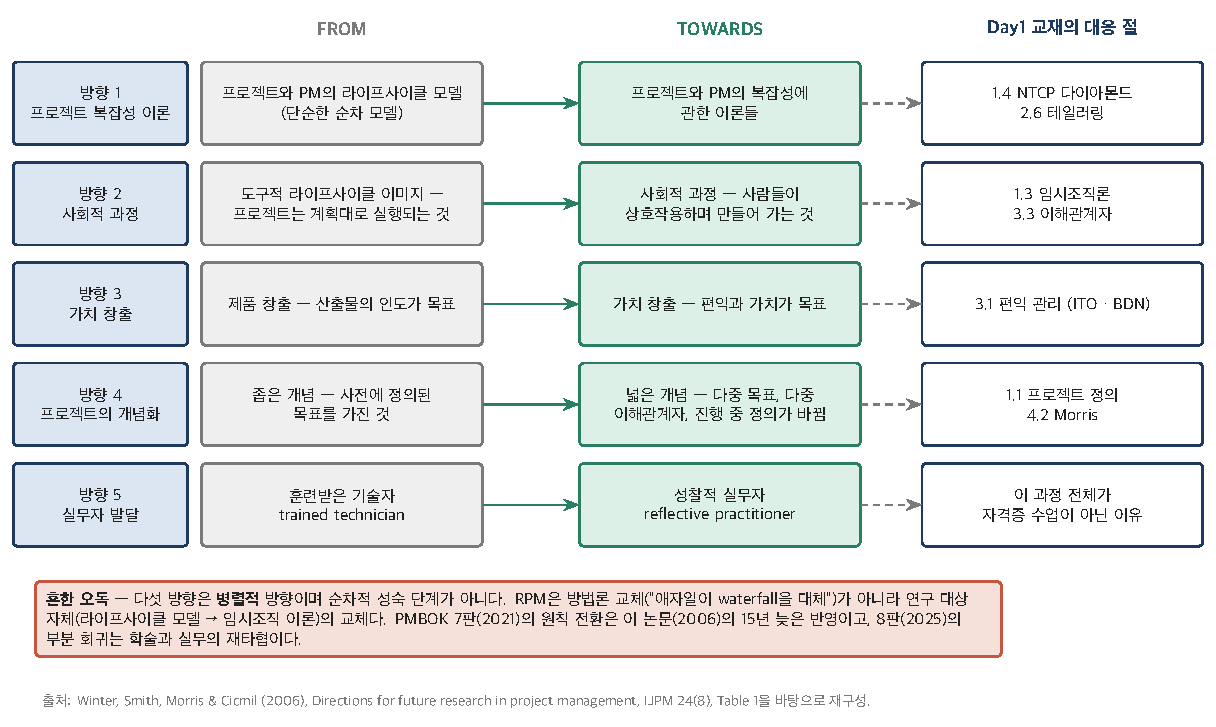
\includegraphics[width=1.00\textwidth,height=0.72\textheight,keepaspectratio]{../그림/PM_Day1/fig_4_1_rpm.pdf}
\par\nobreak\vspace{1pt}{\scriptsize\color{mDarkTeal!70}그림 4-1. Rethinking PM 다섯 방향 FROM$\rightarrow$TOWARDS + Day1 대응 절\par}
\end{center}
\framebreak
{\usebeamercolor[fg]{normal text}\footnotesize\setlength{\tabcolsep}{3pt}\renewcommand{\arraystretch}{1.12}
\begin{tabular}{@{}>{\raggedright\arraybackslash}p{0.087\textwidth}>{\raggedright\arraybackslash}p{0.087\textwidth}>{\raggedright\arraybackslash}p{0.237\textwidth}>{\raggedright\arraybackslash}p{0.340\textwidth}>{\raggedright\arraybackslash}p{0.234\textwidth}@{}}
\toprule
\textbf{\#} & \textbf{방향} & \textbf{FROM} & \textbf{TOWARDS} & \textbf{오늘 어디에} \\
\midrule
1 & 복잡성 이론 & 단순한 순차 라이프사이클 모델 & 프로젝트·PM의 복잡성 이론들 & §1.4 NTCP, §2.6 테일러링 \\
2 & 사회적 과정 & 계획대로 실행되는 도구적 이미지 & 사람들이 상호작용하며 만들어 가는 것 & §1.3 임시조직, §3.3 이해관계자 \\
3 & 가치 창출 & 산출물의 인도 & 편익과 가치 & §3.1 편익 관리 \\
4 & 개념화 & 사전 정의된 목표를 가진 좁은 개념 & 다중 목표·다중 이해관계자·진행 중 정의가 바뀌는 넓은 개념 & §1.1, §4.2 Morris \\
5 & 실무자 발달 & 훈련받은 기술자 (trained technician) & \textbf{성찰적 실무자} (reflective practitioner) & 이 과정 전체가 자격증 수업이 아닌 이유 \\
\bottomrule
\end{tabular}}
\par\smallskip
\begin{itemize}
\item\relax 2003년 EPSRC 연구 네트워크 $\rightarrow$ 2006 IJPM 24(8) 특집. Winter, Smith, Morris, Cicmil의 대표 논문 12페이지
\item\relax 실무적 가치: \textbf{표준 변경을 뉴스가 아니라 사조로 보게 해 준다} — 7판(2021)은 이 논문의 15년 늦은 반영, APM BoK 7판(2019)이 그 사이, 8판(2025)은 학술과 실무의 재타협
\item\relax 흔한 오독: "애자일이 waterfall을 대체했다"는 서사로 축약 / 다섯 방향을 순차 성숙 단계로 / "성찰"을 회고 회의로 등치(Schön의 reflection-in-action은 실시간 판단 습관) / 자격증 무용론으로 — 원 논문은 대체가 아니라 \textbf{발달 경로}
\end{itemize}
\note{§4.1. 같은 특집호의 Cicmil et al.(actuality of projects)과 Crawford et al.(practitioner development)을 한 줄씩. 읽을 것: Winter et al.(2006) 전체, 특히 Table 1. 그다음 Geraldi \& Söderlund(2018). 예상 소요 4분.}
\end{frame}

% ---- md slide 84: Morris — "project management"에서 "the management of projects"로
\begin{frame}[allowframebreaks=1.0]{Morris — "project management"에서 "the management of projects"로}
\small
\begin{itemize}
\item\relax Morris(1994, 『The Management of Projects』)가 바꾼 어법 하나: 전자는 실행 통제(계획·감시·변경 통제), 후자는 프로젝트가 정의되는 \textbf{앞단(front-end)}, 기술, 상업, 정치까지. 성패는 대부분 앞단에서 결정되는데 \textbf{지식체계(BOK)는 실행만 다룬다}
\item\relax Morris(2013, 『Reconstructing Project Management』) — 표준 지식체계가 왜 front-end를 배제하게 되었는가의 계보
\item\relax \textbf{Samset \& Volden(2016)의 열 가지 역설} 중 핵심: \textbf{정보의 가치가 가장 큰 시점에 예산·권한·데이터가 가장 적다.} 착수 전 결정(무엇을, 어느 대안, 어느 규모)은 실행 중 어떤 최적화로도 되돌릴 수 없는데, 그 시점에는 정보도 자원도 없다
\item\relax Flyvbjerg의 break-fix model이 메커니즘 — 앞단이 부실하면 실행에서 반복적 파손과 수리, 그 수리 비용이 원가 초과의 실체. "실행을 잘하자"에는 한계선이 있고 그 선은 앞단에서 그어진다
\item\relax 한국 조직에서 PM은 품의서 결재 뒤에 지명된다. PM 개인이 바꿀 수 없지만 둘은 할 수 있다: ① 착수 시점에 앞단의 결정을 목록화하고 가정·리스크를 헌장에(Engwall) ② 종료 보고서에 "앞단에서 결정된 X가 실행 중 Y의 원인"을 기록해 다음 프로젝트에서 앞단에 들어갈 근거를 만든다
\item\relax 오독: front-end를 "기획 문서 강화"로 — 요점은 문서량이 아니라 의사결정 권한과 \textbf{대안 유지}. front-end 강화를 "착수 지연"으로 — 처방은 think slow, \textbf{act fast}
\end{itemize}
\note{§4.2. 오늘 헌장의 가정 목록을 길게 쓰라고 한 이유가 이것이다 — "착수 시점에 잘못 적힌 것은 계획 시점에 고쳐지지 않는다"(교재 맺음말). 읽을 것: Morris(2013) Part 1·3, Samset \& Volden(2016) 역설 목록 먼저. 예상 소요 4분.}
\end{frame}

% ---- md slide 85: Flyvbjerg — 착각(delusion)과 기만(deception), 그리고 think slow, act fast
\begin{frame}[allowframebreaks=1.0]{Flyvbjerg — 착각(delusion)과 기만(deception), 그리고 think slow, act fast}
\small
\begin{itemize}
\item\relax Flyvbjerg, Garbuio \& Lovallo(2009, CMR) — 예측이 틀리는 이유를 \textbf{두 개의 별개 모델}로
\par\nobreak
\begin{itemize}
\item\relax \textbf{Delusion(착각)} — 심리학: 낙관 편향, 계획 오류, 내부 시각. 진심으로 잘될 것이라 믿는다 $\rightarrow$ 처방: 교육, outside view, RCF
\item\relax \textbf{Deception(기만)} — 정치·경제: 전략적 왜곡(strategic misrepresentation) — 승인받기 위해 원가를 낮추고 편익을 높인다 $\rightarrow$ 처방: 교육이 아니라 \textbf{인센티브·책임·리스크 자본 구조의 설계}
\end{itemize}
\item\relax 2021 PMJ 「Top Ten Behavioral Biases」 1위는 optimism bias가 아니라 \textbf{strategic misrepresentation}. "behavioral bias = cognitive bias"는 오류, 절반은 political bias $\rightarrow$ 편향 교육 워크숍으로 정치 문제를 풀려는 헛수고. 반대 오용: 모든 낙관 견적을 거짓말로 규정해 신뢰 파괴
\item\relax 2002 「Error or Lie?」 $\rightarrow$ 2009 「Survival of the Unfittest」 — 선정되는 것은 최고의 프로젝트가 아니라 \textbf{서류상 가장 좋아 보이는 프로젝트} = 원가 최소·편익 최대로 추정한 프로젝트 = 최악의 프로젝트
\item\relax 온담: 물류 96억의 분모 부재, "4,200은 현장 숫자가 아니다" — 착각인가 기만인가? \textbf{알 수 없고 알 필요도 없다. 처방이 같다} — 편익 프로필에 분모·측정 방법·오너 실명을 요구하고, 없는 항목은 합계에서 제외. CFO의 "근거 없는 항목은 승인 안 함"이 정확히 Flyvbjerg의 제도 처방
\item\relax \textbf{Think slow, act fast}(2023, 『프로젝트 설계자』) — 앞단에 시간을 충분히, 실행은 짧게(실행이 길수록 예상치 못한 사건의 창이 넓어진다). 학습곡선을 타는 것은 \textbf{반복 가능한 동일 단위}(platform, modularity) — P1에서 615개 매장 배포는 모듈화 가능(파일럿 12개점$\rightarrow$확대), 데이터 전환 7.4TB와 컷오버 34시간은 bespoke $\rightarrow$ 리스크는 여기에 집중, 그 앞에 "천천히 생각하는" 시간(리허설 3회, G2·G3)
\item\relax 반대편도 알아야 한다: Hirschman의 \textbf{Hiding Hand}(1967) — Flyvbjerg(2016)가 p<0.0001로 기각(방법론 비판: 11개 성공 사례만 골라 표본 — sampling on the dependent variable) $\rightarrow$ Ika(2018) 반박 $\rightarrow$ Kreiner(2020) "쟁점은 데이터가 아니라 존재론"
\end{itemize}
\note{§4.3. "Flyvbjerg에 따르면"이라고 말할 때 그 반대편이 무엇인지도 말할 수 있는 실무자. 읽을 것: 입문 『프로젝트 설계자』 전체, 숫자는 2014 PMJ(arXiv 1409.0003)·2021 PMJ(arXiv 2202.00125) 무료, IT 청중 배포용은 2011 HBR 3페이지(arXiv 1304.0265). 예상 소요 5분.}
\end{frame}

% ---- md slide 86: Staw — 몰입의 상승(escalation of commitment)과 결정자의 분리
\begin{frame}[allowframebreaks=1.0]{Staw — 몰입의 상승(escalation of commitment)과 결정자의 분리}
\small
\begin{center}\usebeamercolor[fg]{normal text}
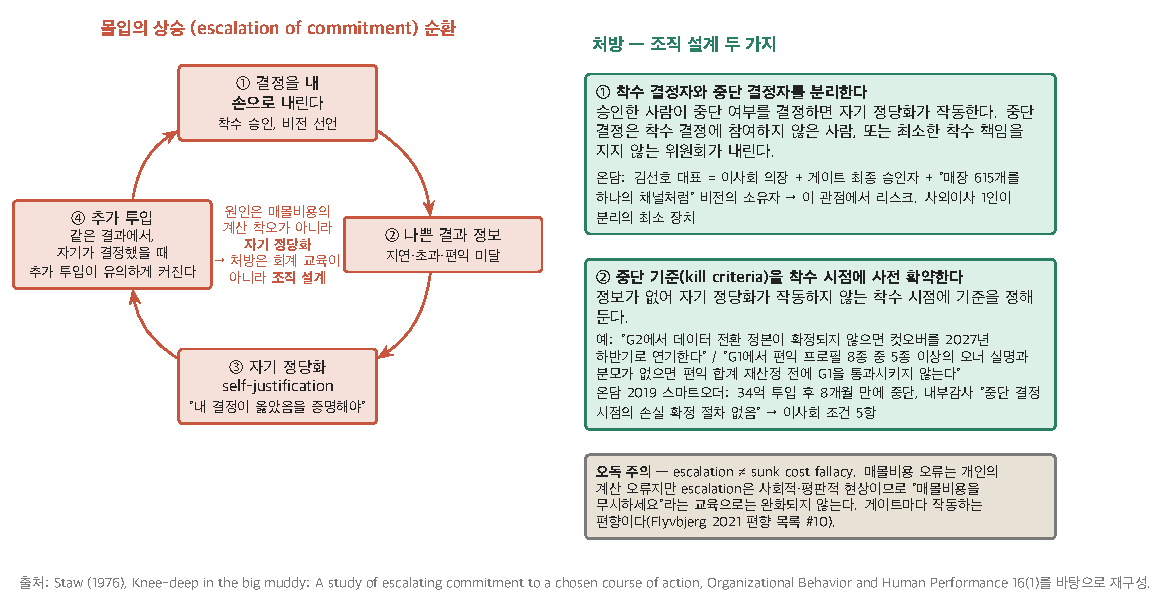
\includegraphics[width=1.00\textwidth,height=0.72\textheight,keepaspectratio]{../그림/PM_Day1/fig_4_4_staw.pdf}
\par\nobreak\vspace{1pt}{\scriptsize\color{mDarkTeal!70}그림 4-2. Staw 몰입의 상승 순환과 두 가지 조직 설계 처방\par}
\end{center}
\framebreak
\begin{itemize}
\item\relax Staw(1976, 「Knee-deep in the big muddy」) 실험: R\&D 예산을 두 사업부 중 하나에 배분 $\rightarrow$ 나쁜 결과 $\rightarrow$ 다시 배분. 조건: 첫 배분을 \textbf{자기가} 했는가 vs 남이 한 것을 이어받았는가
\item\relax 결과: \textbf{동일한 나쁜 결과에서, 그 결정을 자기가 내렸을 때 추가 투입이 유의하게 커진다} $\rightarrow$ 원인은 매몰비용 계산 착오가 아니라 \textbf{자기 정당화(self-justification)}
\item\relax 원인이 자기 정당화라면 처방은 회계 교육("매몰비용을 무시하세요")이 아니라 \textbf{조직 설계} 둘
\par\nobreak
\begin{enumerate}
\item\relax \textbf{착수 결정자와 중단 결정자를 분리한다} — 승인한 사람이 중단을 결정하면 자기 정당화가 작동. 온담: 김선호 대표가 이사회 의장이자 게이트 최종 승인자이자 "615개 매장을 하나의 채널처럼"의 소유자 $\rightarrow$ G1·G2에서 중단해야 할 상황이 오면 그 결정을 대표가 내릴 수 있겠는가. 사외이사 1인이 최소 장치
\item\relax \textbf{중단 기준(kill criteria)을 착수 시점에 사전 확약} — "G2에서 정본이 확정되지 않으면 컷오버를 2027 하반기로", "G1에서 편익 프로필 8종 중 5종 이상의 오너·분모가 없으면 통과시키지 않는다". 정보가 없어 자기 정당화가 작동하지 않는 착수 시점에 정한다. 2019 스마트오더 감사 지적 "중단 시 손실 확정 절차 없음" — 이사회 조건 5항의 핵심이 이것
\end{enumerate}
\item\relax 오독: escalation = sunk cost fallacy — 매몰비용 오류는 개인의 계산 오류, escalation은 \textbf{사회적·평판적 현상}이라 교육으로 완화되지 않는다 / 항상 비합리로 규정 — 정보가 갱신되어 계속하는 것이 옳은 경우와 구별 / Flyvbjerg 2021 편향 목록 \#10 — 착수만이 아니라 \textbf{게이트마다} 작동
\end{itemize}
\note{§4.4. 4교시 헌장 항목 14(조기 종료 조건, 손실 확정 절차)와 5교시 NPD "kill 0건이면 고장"의 학술 근거. 생각해 볼 질문 5(P1을 G1에서 중단할 수 있는가, 기준은, 누가). 읽을 것: Staw(1976) Method 절, Flyvbjerg(2021) \#10. 예상 소요 4분.}
\end{frame}

% ---- md slide 87: 읽을 자료 — 필수 · 30일 · 90일 · 참고 (제5장)
\begin{frame}[allowframebreaks=1.0]{읽을 자료 — 필수 · 30일 · 90일 · 참고 (제5장)}
\small
\par\smallskip\noindent{\usebeamercolor[fg]{normal text}\textbf{필수 (과정 전, 총 90분)} — 사례 회사 문서 §1\textasciitilde{}3·§5 / Klein(2007) 프리모템 2페이지 / 교재 §2.1 연표·§2.2 표 / Cooke-Davies(2002) 6페이지\par}\nobreak
\par\smallskip\noindent{\usebeamercolor[fg]{normal text}\textbf{30일 안에 — Day1에서 열린 질문을 닫는 것}\par}\nobreak
{\usebeamercolor[fg]{normal text}\footnotesize\setlength{\tabcolsep}{3pt}\renewcommand{\arraystretch}{1.12}
\begin{tabular}{@{}>{\raggedright\arraybackslash}p{0.493\textwidth}>{\raggedright\arraybackslash}p{0.492\textwidth}@{}}
\toprule
\textbf{자료} & \textbf{왜} \\
\midrule
Flyvbjerg \& Gardner, 『프로젝트 설계자』(한국경제신문, 2024) & "우리 회사 base rate은 어디서 구하나"로 남은 질문. 8시간 \\
Winter et al.(2006), IJPM 24(8) & 다섯 방향 — 표준 변경을 사조로 \\
Lundin \& Söderholm(1995) / Engwall(2003) & 4T·4행위 / 착수의 진짜 일이 "이미 결정된 것의 목록화"인 이유 \\
Zwikael \& Smyrk(2011) ITO 장 & 워크북 편익 프로필 "오너 실명" 칸의 이론 원전 \\
Eveleens \& Verhoef(2010) 7페이지 & 제안서에서 CHAOS 수치를 빼야 하는 이유를 데이터로 \\
Mitchell, Agle \& Wood(1997) 7유형 정의 절 & 워크북 §3 분류 근거 \\
\bottomrule
\end{tabular}}
\par\smallskip
\par\smallskip\noindent{\usebeamercolor[fg]{normal text}\textbf{90일 안에 — 자기 조직에 적용할 때} — Shenhar \& Dvir(2007) NTCP / Boehm \& Turner(2003) 5축 / Ward \& Daniel(2012) BDN / Bradley(2010) / PRINCE2 7 (Organizing·Progress·Business case practice) / PMBOK 8판 (Standard 전체, Governance·Finance) / Morris(2013) Part 1·3 / Flyvbjerg(2021) 편향 10\par}\nobreak
\par\smallskip\noindent{\usebeamercolor[fg]{normal text}\textbf{참고 (워크북 쓰다가 손을 뻗을 것)} — ISO 21502:2020 §6.4·§7.12·§5.2 / ISO 21505:2017 / ISO 21506:2024 / PMBOK 6판(사내 조항 번호 원문) / Agile Practice Guide Suitability Filter / Snowden \& Boone(2007) / Mitchell, Russo \& Pennington(1989) / Staw(1976) / P3.express v2.0 / PM² Guide v3.1 / 소프트웨어 진흥법 §50\par}\nobreak
\par\smallskip\noindent{\usebeamercolor[fg]{normal text}\textbf{읽지 않아도 되는 것} — Standish CHAOS 원문($\rightarrow$ Eveleens \& Verhoef) / Stacey matrix 2차 자료($\rightarrow$ Snowden \& Boone) / "PMBOK 7판 요약" 류 시중 교재(현행은 8판)\par}\nobreak
\note{§4.5와 제5장. 서지는 교재 §4.5·§5.1\textasciitilde{}5.3과 \textsf{05\_리딩리스트/00\_리딩리스트.md}의 검증 표기를 따른다. arXiv 번호가 있는 것은 무료. 한국어판 표기가 없는 것은 확인되지 않은 것이며 없다는 증명이 아니다. Kahneman \& Tversky 1979 수록지 등 일부 서지는 2차 출처 확인이므로 논문 인용 시 원문 대조. 예상 소요 4분.}
\end{frame}

% ---- md slide 88: 오늘 만든 산출물 다섯 가지
\begin{frame}[allowframebreaks=1.0]{오늘 만든 산출물 다섯 가지}
\small
{\usebeamercolor[fg]{normal text}\footnotesize\setlength{\tabcolsep}{3pt}\renewcommand{\arraystretch}{1.12}
\begin{tabular}{@{}>{\raggedright\arraybackslash}p{0.086\textwidth}>{\raggedright\arraybackslash}p{0.202\textwidth}>{\raggedright\arraybackslash}p{0.086\textwidth}>{\raggedright\arraybackslash}p{0.369\textwidth}>{\raggedright\arraybackslash}p{0.242\textwidth}@{}}
\toprule
\textbf{\#} & \textbf{산출물} & \textbf{워크북} & \textbf{PRINCE2 7 대응} & \textbf{상태} \\
\midrule
① & 비즈니스 케이스 요약 & §1 & Outline Business Case (Project Brief 내) & v0.9 — G1(2026-04-30)에 v1.0 확정 \\
② & 프로젝트 헌장 & §2 & Project Brief $\rightarrow$ PID(핵심부) & v1.0 — 프리모템 반영 후 v1.1 \\
③ & 이해관계자 등록부 + 현저성 분석 & §3 & Communication management approach의 이해관계자 분석부 & G0 판정 — G1·2026-08·G2·G3 갱신 \\
④ & 거버넌스 구조 + RACI 초안 & §4 & Project management team structure, Role descriptions & 허용범위 3층은 Day2 확정 \\
⑤ & 프리모템 기록 + 초기 리스크 목록 & §5 & Risk register(초기), Risk management approach(초안) & 13+2건 정성 — Day2에서 확률·영향·EMV \\
\bottomrule
\end{tabular}}
\par\smallskip
\begin{itemize}
\item\relax 다섯 문서 모두 \textbf{"결정되지 않은 것을 결정하는 문서"}다. Day2 이후의 문서는 Day1에서 결정된 것을 분해하고 측정한다 — \textbf{헌장의 한 줄이 모호하면 WBS 열 개가 모호해진다}
\item\relax 오늘 완성하지 못한 항목은 예시본(§1.5·§2.5·§3.5·§4.5·§5.5)과 대조하며 사후에 채운다. 내일 가져오라
\end{itemize}
\note{워크북 §0.2 표의 Day1 부분. 워크북 §0.1 사용법 10번 — "Day1 산출물은 Day2 계획 산출물의 입력이다. 오늘 쓴 것을 버리지 말고 내일 가져오라." 예상 소요 3분.}
\end{frame}

% ---- md slide 89: 사후 읽기 과제 (Day2까지)
\begin{frame}[allowframebreaks=1.0]{사후 읽기 과제 (Day2까지)}
\small
\par\smallskip\noindent{\usebeamercolor[fg]{normal text}\textbf{읽기}\par}\nobreak
\begin{itemize}
\item\relax Klein(2007) 「Performing a Project Premortem」 — 2페이지. 왜 "실패할 수 있다면"이 아니라 "실패했다"인지를 원문에서 확인 (오늘 실습 전에 못 읽었다면 반드시)
\item\relax Cooke-Davies(2002) 「The 'real' success factors on projects」 — 6페이지. 헌장 항목 3의 두 층이 왜 분리되어야 하는지
\item\relax 교재 제3장 §3.2 "항목별 의미"와 §3.4 "권한 없는 PM" — 오늘 쓴 헌장 항목 12를 다시 읽으며
\end{itemize}
\par\smallskip\noindent{\usebeamercolor[fg]{normal text}\textbf{쓰기 (심화 과제, 3\textasciitilde{}7년차 — 셋 중 하나)}\par}\nobreak
\begin{itemize}
\item\relax 워크북 §1.7: 최근 프로젝트 승인 문서의 편익 표를 항목 4 형식(분모·기여 구분·측정 책임자)으로 다시 쓰고, 분모 없는 항목 / 부서명 책임자 / 남의 편익을 자기 것으로 적은 항목의 개수를 세라
\item\relax 워크북 §2.7: 자기 회사 헌장에서 \textbf{항목 12(PM 권한·허용범위)와 14(완료·중단 기준)}가 없다면 그 둘만 써서 스폰서에게 보여 줄 초안 — Day2 시작 때 한 문장씩 공유
\item\relax 워크북 §4.7: 자기 회사 운영위 명단에 Executive / Senior User / Senior Supplier 배정 — 배정 안 되는 인물 수와 빈 역할
\item\relax 워크북 §5.7: 자기 프로젝트의 실패 선언문 세 개(일정·편익·중단)를 과거형으로, 각 5개 사유 — 현재 리스크 등록부에 없는 것의 개수
\end{itemize}
\par\smallskip\noindent{\usebeamercolor[fg]{normal text}\textbf{기본 과제 변형 (시간이 남는 조)} — §1.7 CFO 148억 확정·P1 2026년 집행 102$\rightarrow$86억 시 항목 5·6 재작성(이월 vs 총예산 152억 축소, 후자면 do-minimum이 되살아나는가) / §2.7 대표의 "컷오버를 2026-11로" 요구 시 항목 13·9·10 재작성과 스폰서 제시 대안 세 개\par}\nobreak
\par\smallskip\noindent{\usebeamercolor[fg]{normal text}\textbf{생각해 볼 질문 (교재 각 장 끝)} — 한 장에 하나씩 골라 답을 적어 오라\par}\nobreak
\begin{itemize}
\item\relax 제1장 3: 온담 2019 스마트오더는 예산 안에서 중단됐다. 이것은 실패인가. 어느 정의로 실패인가
\item\relax 제2장 3: 여러분 프로젝트에서 되돌릴 수 없는 결정은 무엇이고, 그 앞에 얼마나 시간을 쓰고 있는가
\item\relax 제3장 1: 여러분의 마지막 프로젝트에서 편익 오너는 누구였는가. 그 사람은 프로젝트가 끝난 뒤에도 그 조직에 있었는가
\end{itemize}
\note{읽기 과제는 총 1시간 안. 심화 과제는 세 개 중 하나만 해도 된다. 생각해 볼 질문의 답은 Day2 첫 10분에 두세 명이 말한다. 예상 소요 2분.}
\end{frame}

% ---- md slide 90: Day2 예고 — 계획: 범위 · 일정 · 원가 기준선
\begin{frame}[allowframebreaks=1.0]{Day2 예고 — 계획: 범위 · 일정 · 원가 기준선}
\small
{\usebeamercolor[fg]{normal text}\footnotesize\setlength{\tabcolsep}{3pt}\renewcommand{\arraystretch}{1.12}
\begin{tabular}{@{}>{\raggedright\arraybackslash}p{0.212\textwidth}>{\raggedright\arraybackslash}p{0.773\textwidth}@{}}
\toprule
\textbf{Day2 산출물} & \textbf{Day1에서 받는 입력} \\
\midrule
⑥ 범위 기술서와 WBS & 헌장 §5 범위(포함·제외·경계 조건), §6 산출물 — 포함 5개 산출물이 WBS 레벨 2. \textbf{PBS 노드는 명사}(PRINCE2 Product-Based Planning) \\
⑦ 요구사항 추적표(RTM) 골격 & 헌장 §4 상위 요구사항(요구 제공자), §13 우선순위 $\rightarrow$ MoSCoW \\
⑧ 일정 기준선 & 헌장 §7 마일스톤(외부 고정), §9 제약(성수기 창, 규제 기한) $\rightarrow$ 컷오버·규제에서 역산한 주공정, G3 합류 버퍼 15영업일 \\
⑨ 원가 기준선과 예비비 구조 & BC §5 비용·3층 예산, 헌장 §8, RACI 19·20행 $\rightarrow$ 145.8 / 컨틴전시 10.2 / 관리예비비 12.0. R-04(1차연도 삭감) 시나리오별 축소안 \\
⑩ 리스크 등록부 정량화 + 허용범위 격자 & 초기 리스크 13+2건, 허용범위 초안, 손익분기 66\% $\rightarrow$ 확률·영향·EMV, EMV 합계 vs 8억, 편익 $-$5\%p의 타당성 역산 \\
\bottomrule
\end{tabular}}
\par\smallskip
\begin{itemize}
\item\relax Day2에서 다시 만나는 Day1 개념: \textbf{RCF}(원가 기준선의 base rate) / \textbf{멱함수 분포}(컨틴전시가 꼬리를 못 덮는 이유, 처방은 modularity) / \textbf{되돌림 비용}(G2·G3 앞의 예측형 요소) / \textbf{Product-Based Planning}(활동 WBS vs 산출물 PBS) / \textbf{허용범위 격자}(EMV 8억, 원가 +6\%)
\item\relax Day3 실행·통제(변경·리스크·성과 — 3층 변경 통제의 비용, Kreiner의 표류 역설), Day4 종료·이관(검수·운영 전환·편익 검토 — 판본이 바뀌어도 살아남는 산출물, ITIL)
\end{itemize}
\note{워크북 §7 표. Day2에서 Day1 문서로 되돌아오는 것(WBS에서 발견되는 헌장에 없던 산출물 $\rightarrow$ v1.1 범위 수정 요청 / EMV 합계 초과 $\rightarrow$ 허용범위·예비비 재협상)을 말하고 마친다. 교재 맺음말 — "착수 시점에 잘못 적힌 것은 계획 시점에 고쳐지지 않는다. 그것이 Morris가 말한 front-end의 무게이며, 여러분이 오늘 헌장의 가정 목록을 길게 쓰는 이유다." 예상 소요 4분.}
\end{frame}
